\documentclass[12pt,openany]{book}
\usepackage{lmodern}
\usepackage{setspace}
\setstretch{1.25}
\usepackage{amssymb,amsmath}
\usepackage{ifxetex,ifluatex}
\usepackage{fixltx2e} % provides \textsubscript
\ifnum 0\ifxetex 1\fi\ifluatex 1\fi=0 % if pdftex
  \usepackage[T1]{fontenc}
  \usepackage[utf8]{inputenc}
\else % if luatex or xelatex
  \ifxetex
    \usepackage{mathspec}
  \else
    \usepackage{fontspec}
  \fi
  \defaultfontfeatures{Ligatures=TeX,Scale=MatchLowercase}
\fi
% use upquote if available, for straight quotes in verbatim environments
\IfFileExists{upquote.sty}{\usepackage{upquote}}{}
% use microtype if available
\IfFileExists{microtype.sty}{%
\usepackage{microtype}
\UseMicrotypeSet[protrusion]{basicmath} % disable protrusion for tt fonts
}{}
\usepackage[left=4cm, right=3cm, top=3cm, bottom=3cm]{geometry}
\usepackage[unicode=true]{hyperref}
\hypersetup{
            pdfborder={0 0 0},
            breaklinks=true}
\urlstyle{same}  % don't use monospace font for urls
\usepackage{longtable,booktabs}
\usepackage{graphicx,grffile}
\makeatletter
\def\maxwidth{\ifdim\Gin@nat@width>\linewidth\linewidth\else\Gin@nat@width\fi}
\def\maxheight{\ifdim\Gin@nat@height>\textheight\textheight\else\Gin@nat@height\fi}
\makeatother
% Scale images if necessary, so that they will not overflow the page
% margins by default, and it is still possible to overwrite the defaults
% using explicit options in \includegraphics[width, height, ...]{}
\setkeys{Gin}{width=\maxwidth,height=\maxheight,keepaspectratio}
\IfFileExists{parskip.sty}{%
\usepackage{parskip}
}{% else
\setlength{\parindent}{0pt}
\setlength{\parskip}{6pt plus 2pt minus 1pt}
}
\setlength{\emergencystretch}{3em}  % prevent overfull lines
\providecommand{\tightlist}{%
  \setlength{\itemsep}{0pt}\setlength{\parskip}{0pt}}
\setcounter{secnumdepth}{4}
\PassOptionsToPackage{cmyk}{xcolor}
\usepackage[none]{hyphenat}
\usepackage[cmyk]{xcolor} % Recommended by US-AB
\usepackage{lmodern} % Recommended by US-AB
\usepackage{fancyhdr}
\usepackage{etoolbox}
\patchcmd{\chapter}{\thispagestyle{plain}}{\thispagestyle{fancy}}{}{} % Removes plain pagestyle from chapter headings (otherwise, page numbers are centered)
\AtBeginDocument{\addtocontents{toc}{\protect\thispagestyle{empty}}} 
\pagestyle{empty} % This makes ToC without header/footer
\usepackage[skip=15pt]{caption} % This should increase space below captions (not tested)
\raggedbottom
\usepackage[noindentafter]{titlesec}
\usepackage{titlesec}
\titleformat{\chapter}{\normalfont\bfseries}{\thechapter.}{15pt}{}\titlespacing*{\chapter}{0pt}{-50pt}{0pt}
\titleformat{\section}{\normalfont\bfseries}{\thesection.}{1em}{}\titlespacing*{\section}{0pt}{0pt}{0pt}
\titleformat{\subsection}[runin]{\normalfont\bfseries}{\thesubsection.}{1em}{}

\usepackage{CJKutf8} % For Mandarin in Acknowledgments

% For guiding quote in beginning of intro:
\makeatletter
% \renewcommand{\@chapapp}{}% Not necessary...
\newenvironment{chapquote}[2][2em]
  {\setlength{\@tempdima}{#1}%
   \def\chapquote@author{#2}%
   \parshape 1 \@tempdima \dimexpr\textwidth-2\@tempdima\relax%
   \itshape}
  {\par\normalfont\hfill--\ \chapquote@author\hspace*{\@tempdima}\par\bigskip}
\makeatother
\usepackage{placeins}
\usepackage{titlesec}
\usepackage{wrapfig}
\usepackage{caption}
\captionsetup[figure]{font=scriptsize}
\usepackage{float}
\usepackage{subcaption}

\author{}
\date{\vspace{-2.5em}}

\begin{document}

{
\setcounter{tocdepth}{4}
\tableofcontents
}
\cleardoublepage
\pagenumbering{gobble} \pagestyle{fancy} \fancyhf{}
\renewcommand{\headrulewidth}{0pt} \fancyfoot[LE,RO]{\thepage}
\renewcommand{\floatpagefraction}{.9} \setcounter{page}{11}

\chapter*{Abbreviations}\label{abbreviations}
\addcontentsline{toc}{chapter}{Abbreviations}

\begin{longtable}{ll}
\toprule
Abbreviation & Term\\
\midrule
\endfirsthead
\multicolumn{2}{@{}l}{\textit{(continued)}}\\
\toprule
Abbreviation & Term\\
\midrule
\endhead

\endfoot
\bottomrule
\endlastfoot
3' & 3 prime\\
4E-BP & 4E binding protein\\
mcm\textasciicircum{}5s\textasciicircum{}2U & 5-methoxycarbonyl-methyl-2-thiouridine\\
5' & 5 prime\\
A-site & Acceptor-site\\
\addlinespace
ELP3 & Acetyltransferase elongator\\
AMP & Adenosine-mono-phosphate\\
AMPK & Adenosine-mono-phosphate
kinase\\
ATP & adenosine triphosphate\\
APV & Analysis of partial varaince\\
\addlinespace
AUC & Area under the curve\\
ABCE1 & ATP binding cassette protein\\
ChIP & Chromatin immunoprecipitation\\
CR-31 & CR-1-31-B\\
CHX & Cyclohexamide\\
\addlinespace
CTU1/2 & cytosolic thiourdylase 1/2\\
DNA & Deoxyribonucleic acid\\
dsRNA & double-stranded RNA\\
ER & Endoplasmatic reticulum\\
ERalpha & Estrogen receptor alpha\\
\addlinespace
eEF & Eukaryotic elongation factor\\
eIF & Eukaryotic initiation facotr\\
eRF & Eukaryotic release factor\\
E-site & Exit-site\\
GC/MS & Gas chromatography
mass spectrometry\\
\addlinespace
GCN2 & General control nonderepressible 2\\
GLM & Generalised linear model\\
GDP & Guanosine-di-phosphate\\
GTP & Guanosine triphosphate\\
HRI & Heme regulation eIF2alpha kinase\\
\addlinespace
HuR & Human antigen R\\
HIF-1 & Hypoxia inducible factor 1\\
IGF1R & IGF1 receptor\\
IGF1 & insulin-like growth factor 1\\
INSR & insulin receptor\\
\addlinespace
ISR & Integrated stress response\\
LARP1 & La ribonucleoprotein domain family member 1\\
mORF & Main open reading frame\\
mTOR & Mammalian/mechatistic target of rapamycin\\
mRNP & Messenger ribonucleoprotein particle\\
\addlinespace
mRNA & Messenger RNA\\
met-tRNAi & Methionyl-initiatior transfer RNA\\
ALKBH8 & methyltrasnferase TRM9-like domain of alkylation repair homolog 8\\
miRNA & microRNA\\
MAPK & Mitogen-activated protein
kinase\\
\addlinespace
nM & Nano molar\\
NB & Negative binomial\\
ncRNA & non-coding RNA\\
ODC1 & Ornithine decarboxylase\\
PDA & Pancreatic ductal adenocarcinoma\\
\addlinespace
P-site & Peptidyl-site\\
PI3K & Phosphoinositide 3-kinase\\
PABP & Poly A binding protein\\
PIC & Pre-initiation complex\\
PDCD4 & Programmed cell death protein 4\\
\addlinespace
AKT & Protein kinase A\\
PKR & Protein Kinase R\\
PERK & Protein kinase R-like endoplasmatic reticulum kinase\\
RVM & Random variance model\\
ROC & Receiver operating characteristics\\
\addlinespace
RNA & Ribonucleic acid\\
rRNA & Ribosomal RNA\\
RPF & Ribosome protected fragment\\
RBP & RNA binding protein\\
S6K & S6 kinase\\
\addlinespace
sgRNA & single guide RNA\\
TOP & Terminal oligopyrimidine\\
TC & Ternary complex\\
RT-qPCR & Teverse transcription quantitative polymerase chain
reaction\\
tRNA & Transfer RNA\\
\addlinespace
TE & Translation efficiency\\
UTR & Untranslated region\\
uORF & Upstream open reading frame\\
URM & urmylation\\
VEGF & Vascular endothelial growth factor\\*
\end{longtable}

\clearpage
\pagenumbering{arabic} \setcounter{page}{1}

\chapter{Introduction}\section{Gene expression}\subsection{The central dogma of gene expression}

\begin{wrapfigure}{r}{.6\textwidth}
  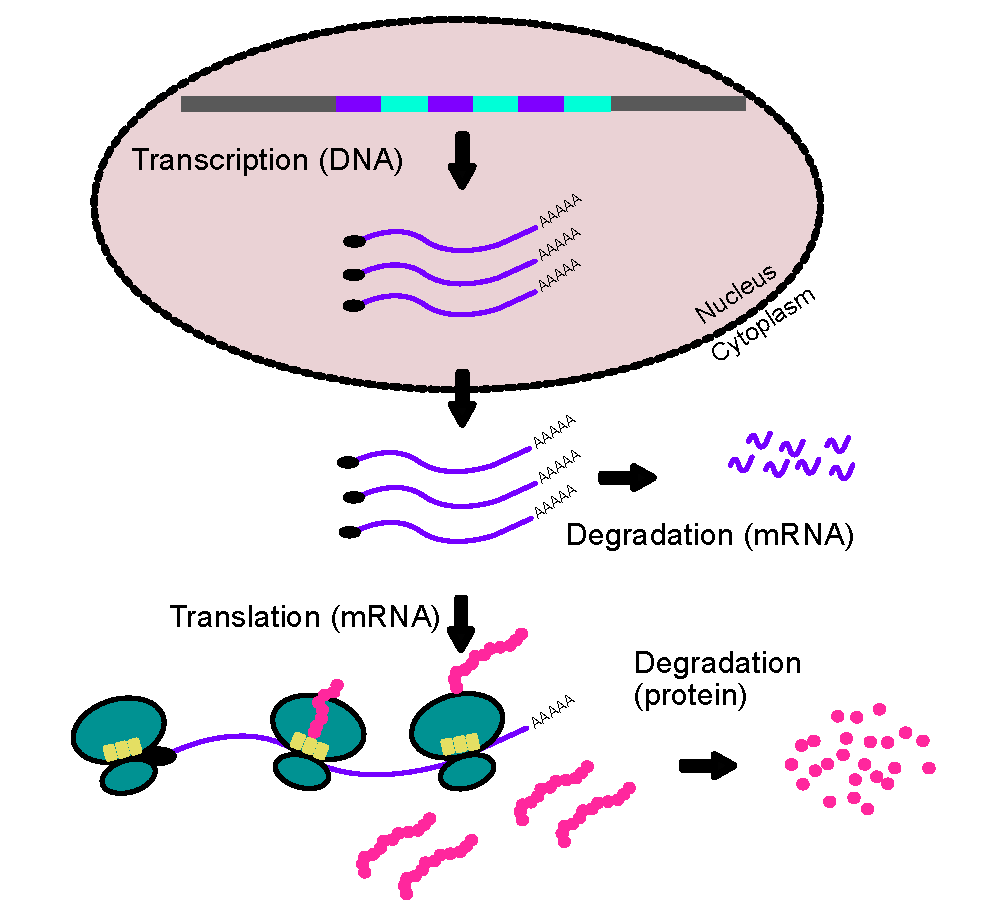
\includegraphics{./figures/geneExprPath_2.pdf}
  \caption{The gene expression pathway - DNA is transcribed into RNA containing a 5' cap (black oval) introns (teal boxes),exons (purple boxes) and a poly(A) tail. RNAs are processed into mRNAs that consisting of a 5' cap, exons and a poly(A) tail. mRNAs can be transported out of the cellular nucleus into the cytoplasm where they can be degraded, stored or translated into proteins depending on cellular demands. Synthesised proteins can be degraded by proteosomes. \label{fig:geneExprPath}}
\end{wrapfigure}

The whole genetic code of an organisms is stored as deoxyribonucleic
acid (DNA) molecules in a double stranded formation as highly condensed
chromosomes. Transcription is the process whereby temporary copies of
the DNA are generated, called transcripts or ribonucleic acid (RNA), and
occurs in the nucleus of eukaryotic cells. RNAs undergo processing by
which multiple different variants coming from the same region are
produced. A subset of protein-encoding processed RNAs is the so called
messenger RNA (mRNA). mRNAs are transported from the nucleus into the
cytoplasm where they can be stored, degraded or translated into
proteins. Proteins themselves can also be degraded. (\textbf{see figure
\ref{fig:geneExprPath}}). This flow of genetic information into
expressed proteins is commonly referred to as the central dogma in
molecular biology (F. Crick, 1970). \clearpage
\subsection{Contribution to gene expression} Proteins are the last
product of the gene expression pathway and carry out the vast majority
of all cellular functions. While it is apparent that modulation of
protein levels will offer information on the changes in gene expression,
it cannot completely answer the question as to why the levels change. In
a disease context, protein levels alone might offer sufficient insight
to explain phenotypic differences. However, information on how these
differences arise mechanistically is obscured. Yet, these differences in
underlying biological mechanisms can be used as targets in therapeutic
strategies.

Recently developed developed system biology methods allow investigation
of gene expression at multiple levels on a genome-wide scale. Initially,
transcriptomics studies were applied to study gene expression with the
assumption that mRNA expression is the main determinant for protein
levels and therefore could be used as a proxy for them. However, this
view was challenged by several landmark studies that observed a poor
mRNA to protein correlation and indicated a larger role of
post-transcriptional regulation in gene expression than previously
assumed (de Sousa Abreu, Penalva, Marcotte, \& Vogel, 2009; J. Lu,
Tomfohr, \& Kepler, 2005; Schwanhäusser et al., 2011; G. M. Silva \&
Vogel, 2016; Vogel \& Marcotte, 2012).

The debate regarding which step of the gene expression pathway
contributes most to the composition of the proteome is ongoing,
nevertheless an understanding has been reached that the context is a
major determinant. At steady state, mRNA levels seem to explain protein
abundance best, however in perturbed systems the contribution of
transcript abundance appears to have less impact relative to
post-transcriptional steps in regulation of gene expression (Y. Liu,
Beyer, \& Aebersold, 2016). For example in a study that stimuleted bone
marrow-derived dendritic cells with LPS, protein levels were dependent
on cellular transcript levels (Jovanovic et al., 2015). In contrast a
study investigating cells under endoplasmatic reticulum stress observed
extensive modulation at the protein levels, whereas mRNA transcript
abundance was only mildly affected (Cheng et al., 2016).

While the contribution of different steps of the gene expression is
dependent on many different factors, e.g.~cellular state or treatments,
mRNA translation (synthesis of proteins) is an essential process in
determining composition of the proteome. Furthermore, dysregulation of
mRNA translation has been observed in multiple diseases, ranging from
neurological disorders to cancer which warrants for a comprehensive
understanding of this process (Graff et al., 2009; Kapur \& Ackerman,
2018; L. J. Lee et al., 2021; Ruggero, 2013). This thesis will focus on
the role of mRNA translation in the context of cancer. \newline
\section{mRNA translation} \subsection{Structure of an mRNA} After
transcription, RNA transcripts are processed into mRNAs. mRNAs contain a
protein coding region which is flanked by untranslated regions (5' and
3' UTRs). UTRs contain post-transcriptional regulatory elements that
effect may affecy localisation, stability and translation of the mRNA
(Leppek, Das, \& Barna, 2018; Loya et al., 2008; Mignone, Gissi, Liuni,
\& Pesole, 2002) (\emph{see figure \ref{fig:UTRFeat}, see also section
\ref{regmRNA} for details}).

\begin{figure}[H]
  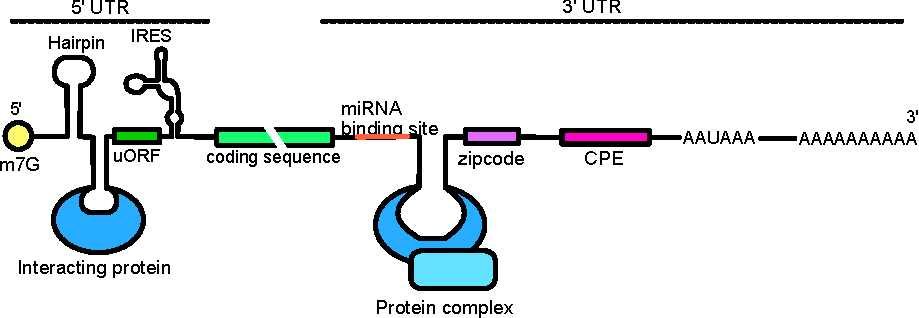
\includegraphics{./figures/UTRFeatures_2.pdf}
  \caption{ Schematic overview of an mRNA- An mRNA consists of a coding sequence, 5' and 3' untranslated regions flanking the coding sequence, a 5' cap and a poly-A tail. Located within the 5' and 3' untranslated region are post-transcriptional regulatory elements that can influence gene expression section \ref{regmRNA} for details. Furthermore, the codon composition of the coding sequence influences translation elongation rates. uORF; upstream open reading frame; IRES, internal ribosome entry site; CPE, cytoplasmic polyadenylation site; AAUAAA, polyadenylation signal.
 \label{fig:UTRFeat}}
\end{figure}

The 5' has a 7-methyl-guanylate (m7G) cap that is important for
translation initiation, while the 3' end has a poly-A tail protecting
the mRNA against degradation (Grifo, Tahara, Morgan, Shatkin, \&
Merrick, 1983; Wilusz, Wormington, \& Peltz, 2001). Multiple different
mRNAs (isoforms or transcript variants) from the same genomic region
exist. These variants may arise due to alternave transcription start
site or a process called alternative splicing which alters the exon
composition (e.g.~coding region) of an mRNA. These variants can co-exist
at the same time and have distinct properties and can perform distinct
functions (Joly Anne-Laure et al., 2018). Furthermore, splicing
resulting in alternative UTRs can introduce differences in translation
for mRNAs encoding the same protein (S. N. Floor \& Doudna, 2016; Jewer
et al., 2020).

\subsection{Translation of an mRNA} \label{translation}

For the vast majority of protein coding mRNAs, eukaryotic mRNA
translation occurs in the cytoplasm, however a small subset of not
nuclear-encoded mRNAs is translated in the mitochondria (D'Souza \&
Minczuk, 2018). mRNA translation is a process that includes initiation,
elongation, termination and ribosome recycling and is an essential
process for protein homeostasis (\textbf{see Figure
\ref{fig:doodlemRNASteps}}). These steps will be discussed in detail
below.

\begin{wrapfigure}{o}{1\textwidth}
  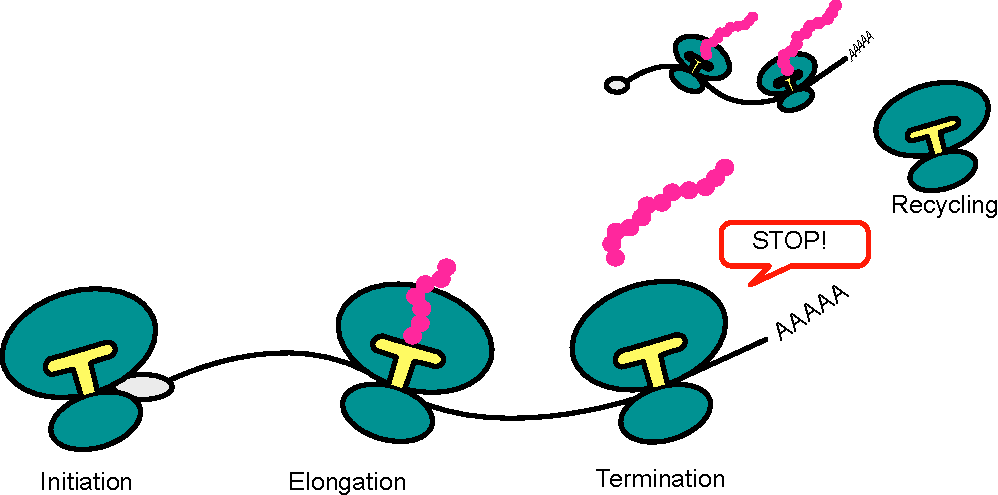
\includegraphics{./figures/doodleTranslation.pdf}
  \caption{mRNA translation initiation, elongation, termination and ribosome recycling steps - The ribosome binds to the mRNA and initiates scanning for a start codon. The elongation phase incorporates amino acids into a polypeptide chain (i.e. the protein product). Once the end of the coding sequence is detected, by recognition of stop codons, the ribosome terminates translation and releases the polypeptide chain. The ribosome can then be recycled to participate in the translation of another mRNA or reinitiate. \label{fig:doodlemRNASteps}}
\end{wrapfigure}

\clearpage

\subsection{Initiation} \label{initiation}

In eukaryotes 5' cap dependent mRNA translation consists of multiple
stages. First, a ternary complex (TC) consisting of GTP bound eukaryotic
initiation factor (eIF) 2 and methionine-initiator tRNA (met-tRNAi) is
formed. This is followed by formation of the 43S pre initiation complex
(PIC) consisting of a 40S ribosome subunit, eIF1, eIF1A, eIF3, eIF5 and
the TC (Asano, Clayton, Shalev, \& Hinnebusch, 2000). mRNAs then
undergoe ``activation'' by which the 5' cap proximal structure is
unwound by eIF4F with eIF4B in an adenosine-tri-phosphate (ATP)
dependent manner. eIF4F is the 5' cap binding complex consisting of;
eIF4E, 5' cap binding protein; eIF4A, an RNA helicase and; eIF4G, a
scaffold protein (Grifo et al., 1983). Poly a binding protein (PABP)
binds in the 3' UTR and causes circularisation of the mRNA to improve
its stability and aid in recruitment of translation initiation factors
(Ivanov et al., 2016). The 43S complex then binds to this unwound region
and starts scanning in the 5' to 3' direction. Recognition of the
translation initiation codon (AUG) induced the 48S initiation complex
formation. Here displacement of eIF1 occurs which allows eIF5 to
hydrolyse eIF2-bound GTP. The 60S subunit then joins the 48S initiation
complex which causes the release of eIF2-GDP and other initiation
factors (eIF1, eIF3, eIF4B, eIF4F and eIF5) and is mediated by eIF5B.
After subunit joining the ribosome starts the elongation process
(\textbf{Figure \ref{initiation}}) (Asano et al., 2000; Hinnebusch,
2006; Jackson, Hellen, \& Pestova, 2010). 5' cap independent mRNA
translation initiation can also occur, e.g.~via the internal ribosome
entry site (IRES) (\emph{Figure \ref{fig:UTRFeat}}). These mechanisms
are extensively reviewed elsewhere (Lacerda, Menezes, \& Romão, 2017).

\subsection{Elongation}

The 80S ribosome contains three sites important for decoding an mRNA:
the aminoacyl (A), peptidyl (P) and exit (E) sites. During elongation in
eukaryotes, aminoacytelated tRNAs are delivered to the A-site in a TC
with eukaryotic elongation factor 1A (eEF1A) and guanosine triphosphate
(GTP). If the tRNA is cognate to the condon in the A-site of the
ribosome, eEF1A is hydrolysed causing its release and accommodating the
tRNA in the A-site. This is followed by a peptidyl transferase reaction
forming the peptide bond by the transfer of the nascent polypeptide from
peptidyl tRNA in the P-site to the amino group of the A-site
aminoacyl-tRNA (aa-tRNA). Then a translocation steps occurs through
eEF2-GTP hydrolysis which translaocates deacetylated tRNA into the
E-site and peptidyl tRNA to the P-site. The deacytelated tRNA is then
released from the ribosome (Dever \& Green, 2012). This process is
repeated until a stop codon (UAA, UGA or UAG) enters the A site of the
ribosome .

\begin{figure}[ht]
\centering
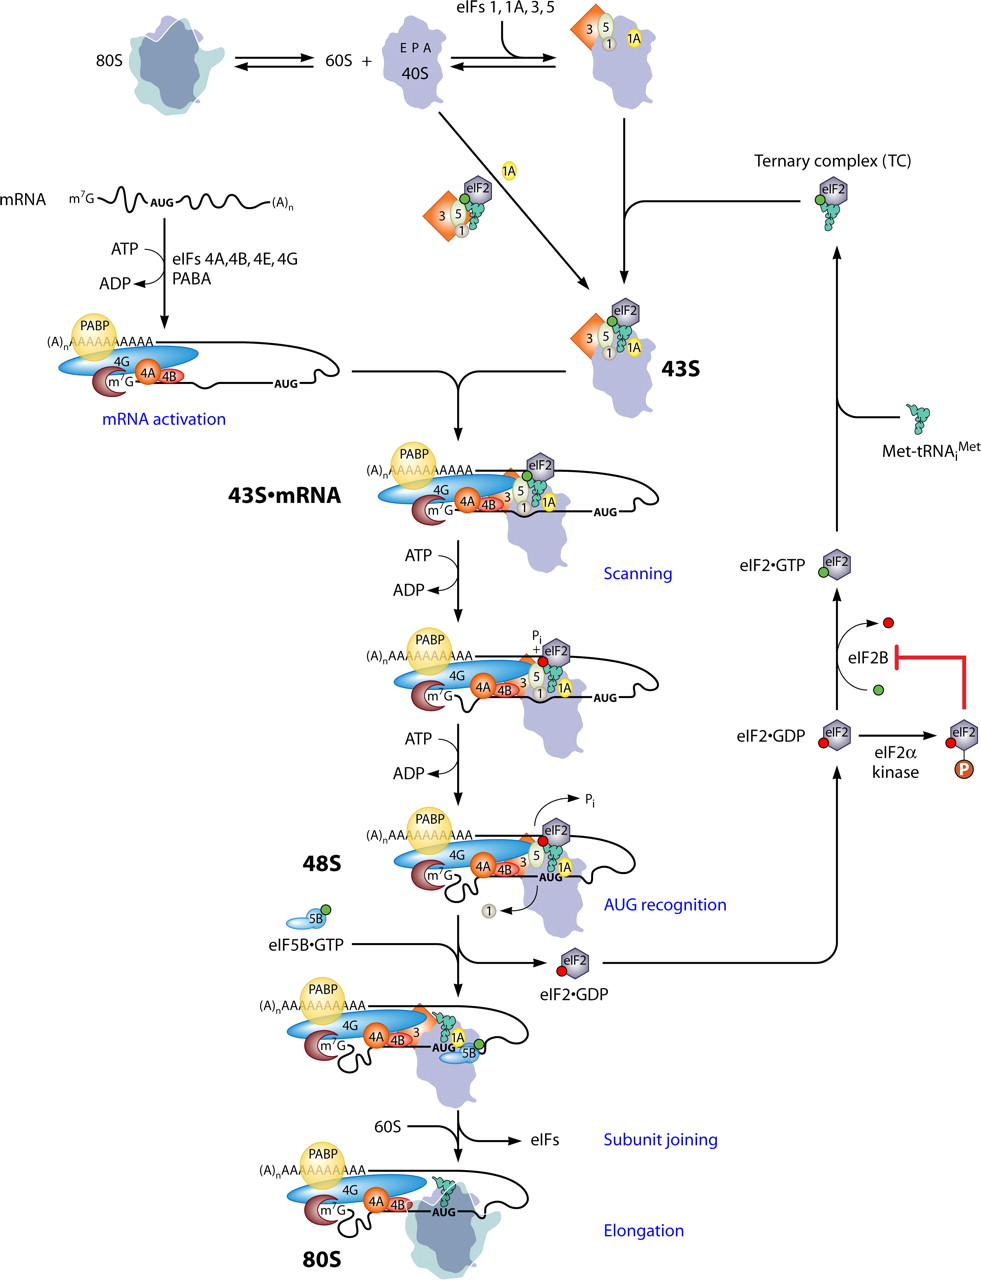
\includegraphics[width=1.0\linewidth,height=0.7\textheight]{./figures/initiation.jpg} 
  \caption{Pathway of eukaryotic translation initiation via ribosomal scanning.
  \label{fig:initiation}}
\end{figure}

\clearpage

\subsection{Termination and recycling}\begin{wrapfigure}{r}{.4\textwidth}
  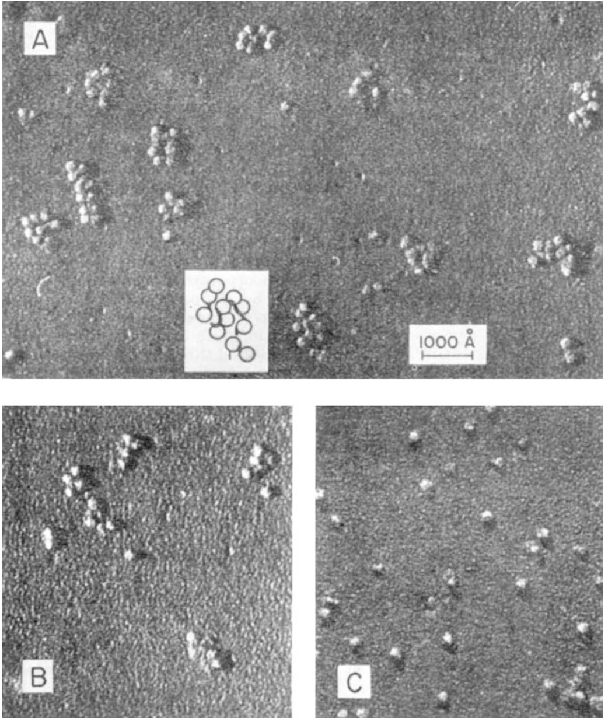
\includegraphics{./figures/polysome.pdf}
  \caption{Electromicrongraph of ribosomes extracted from different positions along a sucrose gradient used for polysome fractionation (A-C). For details on polysome fractionation see section \ref{exptMethod}. Reprinted with permission. DR. T. STAEHELIN et. al. Nature.1963 Aug 31;199:865-70.doi: 10.1038/199865a0. Copyright © 1963, Nature Publishing Group.
  Schematic of the TAPES method - A ribosome (A) can initiate with rate \(\alpha\) on an mRNA with a coding sequence with codons i= 1 ... L. The elongation rate at a specific codon is defined by \(\omega_i\) and \(\beta\) determines the termination rate once a stop codon is encountered. TASEP has been constantly modified, e.g. to allow for correction of initiation or elongation when the following codon is already occupied. Reprinted with permission. Juraj Szavits-Nossan and Martin R. Evans. 10.1103/PhysRevE.101.062404. ©2020 American Physical Society. 
 \label{fig:polysomes}}
\end{wrapfigure}

mRNA translation termination is facilitated by two eukaryotic release
factors (eRF), eRF1 and eRF3-GTP (E. Z. Alkalaeva, Pisarev, Frolova,
Kisselev, \& Pestova, 2006; I. Stansfield et al., 1995). The
eRF2:eRF3-GTP complex binds to the A-site of the ribosome upon
recognition of a stop codon. This causes an hydrolysis event resulting
in a conformational change and release of the polypeptide chain. eRF1
and the ATP binding cassette protein (ABCE1) together promote the
splitting of the 60S and 40S subunits after which they can be recycled
(Hellen, 2018; Pisarev et al., 2010).

\subsection{Translation efficiency}

Each ribosome synthesises a single protein during translation of an mRNA
assuming it is not prematurely terminated. It has been known since the
'60s that translation of an mRNA occurs via multiple bound ribosomes
(polysomes) simultaneaously (\textbf{see figure \ref{fig:polysomes}A-C})
(Staehelin, Brinton, Wettstein, \& Noll, 1963; Warner, Rich, \& Hall,
1962). Therefore the translation efficiency of an mRNA depends on the
number of ribosomes it is associated with. While all steps of
translation can affect the translation efficiency of an mRNA, it is
thought to most commonly be regulated at the initiation step (Dever \&
Green, 2012; Jackson et al., 2010; J. D. Richter \& Coller, 2015).

Experimental methods, e.g.~polysome profiling, are used to study
translation efficiencies. Furthermore, there are efforts to model
translation kinetics such as totally asymmetric simple exclusion process
(TASEP) to obtain a better understanding of ribosome movements along the
mRNA (C. T. MacDonald, Gibbs, \& Pipkin, 1968; Maniloff, 1969)
(\textbf{See figure \ref{fig:polysomes}D}). A model that assessed
ribosome traffic under steady state and high initiation rates indicates
traffic is not only dependent on the densities of ribosomes but also
codon specific elongation rates and their distribution along the mRNA
(Szavits-Nossan \& Evans, 2020). The next section will go further into
detail how initiation rates and elongation can be regulated. \newline
\section{Regulation of mRNA translation} \label{regmRNA}

mRNA translation is the most energy consuming process in the cell. In a
study using concanavalin A stimulated rat thymocytes, it was estimated
that translation accounts for \textasciitilde{}20\% of the cellular
energy consumption (Buttgereit \& Brand, 1995). The high energy
consumption of mRNA translation and its central role in the gene
expression pathway requires it to be tightly regulated, especially in
cancer where dysregulated metabolism is common (Hanahan \& Weinberg,
2011).

Regulation of translation can be exerted at a global level
(i.e.~regulation of a large set of mRNA simultaneously) by
e.g.~perturbations of major signalling pathways impinging on mRNA
translation. Furthermore, a strong feature of translational control is
that it can affect distinct mRNA populations selectively. This form of
translational regulation acts on characteristics of mRNAs, e.g.~through
cis elements in the UTRs, RNA binding proteins (RBP) (\textbf{see figure
\ref{fig:UTRFeat}}) or regulation of initiation factors (Leppek et al.,
2018). Below we will discuss multiple mechanisms that regulate mRNA
translation globally or selectively.

\subsection{mTOR} \label{mTOR}

mTOR is a conserved Ser/Thr kinase and is found in two structurally and
functionally distinct complexes, mTORC1 and mTORC2 (Pearce et al., 2007;
Saxton \& Sabatini, 2017). In a growth promoting environment mTOR
switches cell metabolism to increase protein synthesis, lipids and
nucleotides, while suppressing catabolic pathways, e.g.~autophagy.
mTORC2 promotes survival via signalling through protein kinase A (AKT),
anabolic metabolism, and cytoskeleton regulation (Sarbassov, Guertin,
Ali, \& Sabatini, 2005,Zoncu, Efeyan, \& Sabatini (2011)).

mTOR activity is modulated via hormone and growth factor signalling
(i.e.~insulin and insulin-like growth factor; IGF1). This signalling is
predominantly mediated through the phosphoinositide 3-kinase (PI3K) /
AKT pathway. PI3K activation generates
phosphatidylinositol-3,4,5-trisphosphate (PIP3). This is counteracted by
phosphatase and tensin homologue (PTEN) by hydrolsis of PIP3 to
phosphatidylinositol 4,5-bisphosphate (PIP2). PIP3 recruits
phosphoinositide-dependent kinase 1 (PDK1) and AKT to the plasma
membrane where AKT is activated through phosphorylation of PDK1. AKT in
turn increases activity towards its substrate; tuberous sclerosis
complex (TSC) consisting of TSC1, a scaffold protein and TSC2 a GTPase,
which negativeley regulates mTOR. This negative regulation occurs
through hydrolsis of Ras homologue enriched in brain (Rheb) leading to
its inactivation. Rheb binds to mTOR to promote its activity (\emph{see
Figure \ref{fig:mtorsignal}}). Furthermore, signalling through the
RAS/ERK pathway can also activate mTOR (reviewed here (Reuben J. Shaw \&
Cantley, 2006)).

The PI3K pathway is involved in oncogenic signalling and under
investigation as therapeutic targets in cancer (Hilger, Scheulen, \&
Strumberg, 2002; J. Yang et al., 2019). In several cancers (e.g.~breast,
lung, prostate and colon) the gene encoding the catalytic p110\(\alpha\)
subunit of PI3K (PI3KCA) is frequently mutated or amplified (J. W. Lee
et al., 2005; D. A. Levine et al., 2005; Samuels et al., 2004). The
E545K mutation leads to a reduced inhibition of PI3KCA by p85. In
\textbf{study 3} we investigate oncogenic signalling via the PI3K
pathway activated by insulin and the role of mTOR in mediating the
resulting effects on gene expression in the MCF7 breast cancer cell line
that harbours the E545K mutation (Schneck et al., 2013). Hyperactivity
of PI3K/AKT signalling has been reported in multiple cancers and been
linked anti- cancer therapy resistance (Pópulo, Lopes, \& Soares, 2012;
Salaroglio, Mungo, Gazzano, Kopecka, \& Riganti, 2019; Tan \& Yu, 2013).
Furthermore, both PTEN and the TSC act as tumour suppressors and are
frequently mutated in cancer (Mak \& Yeung, 2004; M. S. Song, Salmena,
\& Pandolfi, 2012). mTOR, as a downstream target of these factors
integrating their signals, has therefore become a focus of anti-cancer
therapy by either targeting mTORC1 or using dual inhibitors for PI3K and
mTOR (Bhat et al., 2015). \clearpage

\begin{figure}[ht]
 \centering
  \includegraphics{./figures/mTORsignal.jpg}
  \caption{Schematic representation of mTOR signaling to the translational machinery. Philippe P. Roux, and Ivan Topisirovic Mol. Cell. Biol. 2018; doi:10.1128/MCB.00070-18. Reprinted with permission. Copyright © 2018, American Society for Microbiology
 \label{fig:mtorsignal}}
\end{figure}

mTOR also fulfills a central role in metabolic signalling where it
integrates amino acid availability, glucose and cellular oxygen levels
to form an appropriate response. For example, increased amino acid
availability induces relocalisation of mTOR into proximity of Rag
GTPases leading to its activation through Rheb (Sancak et al., 2008).
Furthermore, Glucose deprivation leads to increased
adenosine-mono-phosphate kinase (AMPK) signalling via phosphorylation of
serine/threonine kinase 11 (LKB1) (Kimball, 2006; M. J. Sanders,
Grondin, Hegarty, Snowden, \& Carling, 2007; R. J. Shaw, 2009). In turn,
AMPK phosphorylates TSC2 leading to its activation (Kimball, 2006).
LKB1, by activating TSC2, therefore acts as a tumor suppressor.
Furthermore, LKB1 mutations have been found in cancer and is a target of
anti-cancer therapy (R.-X. Zhao \& Xu, 2014). Hypoxia also inhibits mTOR
via regulated in development and DNA damage response 1 (REDD1) which
stabilises the TSC (Brugarolas et al., 2004). While hypoxia
(i.e.~deprivation of oxygen) inhibits protein synthesis in normal cells,
in breast cancer, protein synthesis was not inhibited during hypoxia
which is attributed to uncontrolled mTOR signalling (Connolly,
Braunstein, Formenti, \& Schneider, 2006).

Given the central of mTOR governing proliferation, growth and
metabolism, which are often deregulated in cancer, it is vital to
comprehensively understand mTORC1 signalling herein to better formulate
treatment strategies (Hanahan \& Weinberg, 2011; P. P. Roux \&
Topisirovic, 2018).

\subsubsection{Global regulation of translation via mTOR}

Well studied downstream targets of mTOR for the regulation of mRNA
translation are 4E-binding protein (4E-BP) and ribosomal protein S6
kinases (S6Ks). mTOR phosphorylates 4E-BP leading to the release of
eIF4E that then can engange in eIF4F complex formation (A.-C. Gingras et
al., 1999). Therefore, inhibition of mTOR leads to a down regulation of
cap dependent mRNA translation.

S6Ks have been shown to regulate phosphorylation of multiple components
of the translation machinery, e.g.~ribosomal protein S6 (rpS6),
programmed cell death protein 4 (PDCD4), eEF2 and eIF4B. S6K
phosphorylation rpS6 which has been implicated iin the regulation of
cellular growth and protein synthesis (Ruvinsky et al., 2005).
Furthermore, S6K/rpS6 signalling was suggested to be involed in ribosome
biogenesis. Another S6K target is eEF2 which, as mentioned above,
facilitates transocation of peptidyl-tRNAs and therefore affects
ribosome elongation rates (X. Wang et al., 2001). Furthermore,
phosphorylation of PDCD4 by S6K triggers its degradation. PDCD4 blocks
eIF4G-eIF4A interactions repressing eIF4A activity and cap dependent
mRNA translation (Dorrello et al., 2006; A. Göke et al., 2002). Lastly,
phosphylation of eIF4B by S6K stimulates unwinding activity of eIF4A
(Rogers, Richter, Lima, \& Merrick, 2001).

Collectively, through acting on its downstream targets, mTOR regulates
translation via cap dependent mechanisms, elongation as well as ribosome
biogenesis.

\subsubsection{Selective or "mTOR sensitive" regulation of translation}

Selective or ``mTOR sensitive'' regulation of translation acts on
transcripts with a terminal oligo pyrimidine motif (TOP mRNAs). This TOP
motif consists of a C followed by a stretch of 4-15 pyrimidines directly
after the 5' cap. TOP mRNAs show near complete dissociation from
ribosomes under conditions when mTOR is inhibited and are enriched for
genes encoding for components of the translation machinery (Meyuhas,
2000; Thoreen et al., 2012; Yamashita et al., 2008). Recent works
indicate the importance of La ribonucleoprotein domain family member 1
(LARP1) in regulation of TOP mRNAs with contradictory findings (B. D.
Fonseca et al., 2015; Hopkins et al., 2016; Jia et al., 2021; Maraia,
Mattijssen, Cruz-Gallardo, \& Conte, 2017). A panel of researches were
asked to evaluate these findings which led to the establishment of a
model for translational regulation via LARP1 (Berman et al., 2021).
Herein, LARP1 is thought to bind to the 5' mRNA cap of TOP mRNAs via its
DM15 domain and represses translation by obstructing eIF4E binding in
instances where mTOR activity is abolished. In environments where mTOR
is active phosphorylation of the DM15 occurs by mTOR causing it to
release the 5' cap, wile the la domain of LARP1 remains bound to the
mRNA thereby stabilizing it to facilitate translation (Berman et al.,
2021). Other instances of selective translation are for mRNAs that lack
the TOP motif, but show sensitivity to mTOR activity due to its role in
eIF4F complex formation.

\subsection{selective regulation through members of the eIF4F complex} \label{sel4F}

As mentioned above, the eIF4F complex consists of eIF4E, eIF4A and eIF4G
and is required for cap dependent mRNA translation (A. G. Hinnebusch,
2014). The availability of the eIF4F complex is normally limited due to
the availability of eIF4E. Therefore, under normal conditions mRNAs must
compete for translation. Such competition is affected by characteristics
of 5' UTRs that introduce variation to how well mRNAs can be translated.
Benedetti et. al. derived and expanded on a model for mRNA competition
origally proposed by Lodish (De Benedetti \& Graff, 2004 ; Lodish,
1974). Herein, ``strong'' mRNAs are widely expressed and represent the
majority of cellular mRNAs and are characterised by optimally long and
unstructured 5' UTRs, e.g. \(\beta\)-actin. An optimal 5' UTR length of
\textasciitilde{}80 nucleotides was proposed by Kozak (Kozak, 1987). On
the other hand, weak mRNAs show long and structured 5' UTRs and encode
for potent growth and survival factors, e.g.~c-Myc, ornithine
decarboxylase (ODC1) and vascular endothelial growth factor (VEGF).
Translation of ``strong'' mRNAs would remain effective in conditions
where eIF4F complex availability would be limited. However, ``weak''
mRNAs show sensitivity to eIF4F availability which is dependent on eIF4E
expression (Graff, Konicek, Carter, \& Marcusson, 2008). Elevated eIF4E
expression is common in cancer and drives malignancy due to selective
induction of translation of tumor promoting mRNAs (De Benedetti \&
Graff, 2004).

Studies investigated the effects of eIF4A inhibition on mRNA translation
and the underlying characteristics of eIF4A dependent mRNAs. Therein,
mRNAs that were senstitive to silvesterol treatment showed
characteristics of ``weak'' mRNAs, i.e.~these mRNAs had long and
structured 5' UTRs (Rubio et al., 2014; Waldron, Raza, \& Le Quesne,
2018; Wolfe et al., 2014). Stuctural elemenents in the 5' UTRs include
classical hairpins formed through Watson-Crick basepairing (\emph{see
Figure \ref{fig:UTRFeat}}) (Leppek et al., 2018). Furthermore,
structures using hoogsteen basepairing that form G-quadruplexes have
been proposed to regulate eIF4A dependent mRNA translation (Wolfe et
al., 2014). G-quadruplexes are stable structures formed by stacking two
or more G-tetrads (Kwok \& Merrick, 2017). Yet, whether G-quadrplexes
form in cells is still debated (Biffi, Di Antonio, Tannahill, \&
Balasubramanian, 2014; J. U. Guo \& Bartel, 2016; Laguerre et al., 2015;
Weldon, Eperon, \& Dominguez, 2016). Predictions of G-quadruplex
structures are based on occurrences of \(GGC_4\) motif repeats (Singh et
al., 2021; Wolfe et al., 2014). Indeed, multiple studies report
enrichments of \(GGC_4\) motifs in mRNAs whose translation is dependent
on eIF4A (Modelska et al., 2015; Rubio et al., 2014; Singh et al., 2021;
Waldron et al., 2018). However, Waldron et al. show that \(GCC_4\)
motifs fail to form G-quadruplexes in their reporter mRNA system. The
authors concluded that eIF4A dependence of mRNAs with \(GGC_4\) motifs
enriched in their 5' UTR was likely mediated by classical hairpin-like
structures (Waldron et al., 2018). In addition one third of eIF4A
dependent mRNAs were encoded by genes with multiple 5' UTR variants,
while for eIF4A independent mRNAs this was \textless{} 1\% (Rubio et
al., 2014). Translation of mRNAs with different 5' UTR variants has
recently been implicated to drive cancer cell plasticity towards more
``stem cell like'' phenotypes during hypoxia (Jewer et al., 2020). A
note here is the use of eIF4A inhibitors with different modes of action
in these studies. Hippuristanol inhibits RNA interaction of selective
binding to eIF4A (Bordeleau et al., 2006; Lindqvist et al., 2008). In
contrast rocaglates and its derivatives, e.g.~silvestrol and CR-1-31-B,
clamp eIF4A on polypurine sequences on the mRNA (Iwasaki, Floor, \&
Ingolia, 2016).

Recently, a more nuanced picture for translation of mRNAs sensitive to
inhibition of components of the eIF4F complex has been shown (Gandin et
al., 2016a). Therein, a comparison of treatments with an mTOR inhibitor
(i.e.~limiting eIF4F complex assembly) and silvesterol were evaluated
leading to identification of mTOR-eIF4E and mTOR-eIF4A senstive mRNAs.
Indeed, as shown before mTOR-eIF4A senstive mRNAs were characterised by
long and structured 5' UTRs and endoced for pro surival proteins and
their translation was also dependent on eIF4E availability. mTOR-eIF4E
sensitive mRNAs were similarly to mTOR-eIF4F dependent mRNAs
characterised by long and structured 5' UTRs. However, mTOR-eIF4E
sensitve mRNAs included a subset of mRNAs with short and unstrctured 5'
UTRs. This additional subset consisted of mRNAs encoding for proteins
involved in metabolic functions.

\subsection{The integrated stress response}

The integrated stress response is a pathway which is activated through
kinases responding to various stress signals. These kinases include
Protein kinase R-like endoplasmic reticulum kinase (PERK) which is
activated by misfolded peptides in the endoplasmatic reticulum (ER),
Heme regulated eIF2alpha kinase (HRI) which is activated during
oxidative stress, protein kinase R (PKR) which is activated in response
to certain viral infections by binding to double-stranded RNA (dsRNA)
and general control nonderepressible 2 (GCN2) which is activated when
cells are deprived of amino acids(Dmitry E Andreev et al., 2015; Guan et
al., 2017; Kapur, Monaghan, \& Ackerman, 2017; Lemaire, Lary, \& Cole,
2005; Taniuchi, Miyake, Tsugawa, Oyadomari, \& Oyadomari, 2016). During
the integrated stress response the alpha subunit of eIF2 is
phosphorylated. Phosphorylated eIF2\(\alpha\) directly engages the
guanine nucleotide exchange factor eIF2B and prevents conversion of
inactive eIF2-GDP to active eIF2-GTP needed for met-tRNAi incorporation
in the TC, therefore inhibiting translation by reducing TC availability
(Sonenberg \& Hinnebusch, 2009) (\textbf{see also figure
\ref{fig:initiation}}).

\subsubsection{Global and selective regulation of translation via the ISR}

Global and selective regulation of translation via the ISR is, similar
to mTOR signalling, achieved at a global and selective level.
Phosphorylation of eIF2 alpha limits ternary complex availability,
therefore met-tRNAi recruitment to the ribosome is limited which results
in a reduction of translation initiation. While global translation is
reduced upon ISR, translation of a selective subset of mRNA with
upstream open reading frames (uORFs) is increased. A uORF is a reading
frame that originates in the 5' UTR of an mRNA upstream of the coding
sequence ORF (\emph{see Figure \ref{fig:UTRFeat}}). uORFs can be out of
frame with the main ORF (mORF) and, when translated, lower the
expression of the mORF (Kozak, 1984). Activating transcription factor 4
(ATF4), that regulates expression of stress response genes, contains
multiple uORFs of which one partially overlaps with the mORF. Under
normal conditions ATF4 mRNA translation is initiated at uORF1 and
reinitiation at uORF2 occurs. The overlap of uORF2 with the mORF causes
ribosomes to synthesise protein from uORF2 thereby inhibiting the
translation of the coding sequence. Limitation of TC availability during
ISR causes longer ribosome scanning times leading to that ribosomes scan
past uORF2 and initiate at the mORF (i.e.~delayed reinitiation)
(Pakos-Zebrucka et al., 2016).

Ribosome profiling studies indicate that 50\% of mammalian mRNAs harbour
uORFs (\emph{see section \ref{exptMethod} for detials on ribosome
profiling}). mRNAs containing uORFs include oncogenes and transcripts
important in differentiation and cell cycle (Calvo, Pagliarini, \&
Mootha, 2009; Ingolia, Lareau, \& Weissman, 2011). Apart from delayed
reinitiation, uORF translation can also be due to ``leaky scanning''.
The surrounding sequence of the uORF is important for initiation of
translation. An AUG in the classical Kozak context
(i.e.~RNN\textbf{AUG}G) is most efficient for translation initiation due
to better recognition by the met-tRNAi (Calvo et al., 2009; Kozak,
1986). Unfavored flanking sequences of the AUG can cause the ribosome to
scan past the AUG, this process is called ``leaky scanning''. An example
of this is DNA-inducible gene 34 (GADD34) which increases its
translation upon ER stress (i.e.~conditions where eIF2\(\alpha\) is
phosphorylated). In humans, GADD34 contains two uROFs separated by 30
nucleotides (Y.-Y. Lee, Cevallos, \& Jan, 2009). In contrast to the
uORFs in ATF4, the uORFs in GADD34 cannot promote reinitiation. Under
basal conditions uORF2, which has a poor kozak context, represses
translation of the CDS. However, under stress causing eIF2\(\alpha\)
phosphorylation, ribosomes scan past uORF2 to translate the CDS (Young,
Willy, Wu, Sachs, \& Wek, 2015). Furthermore, other elements
(e.g.~structures) in proximity of the uORF can also influence its
translation (H. Ruan, Hill, Fatemie-Nainie, \& Morris, 1994).

\subsection{Regulation of mRNA translation by tRNAs} \label{tRNA}\begin{wrapfigure}{r}{0.6\textwidth}
  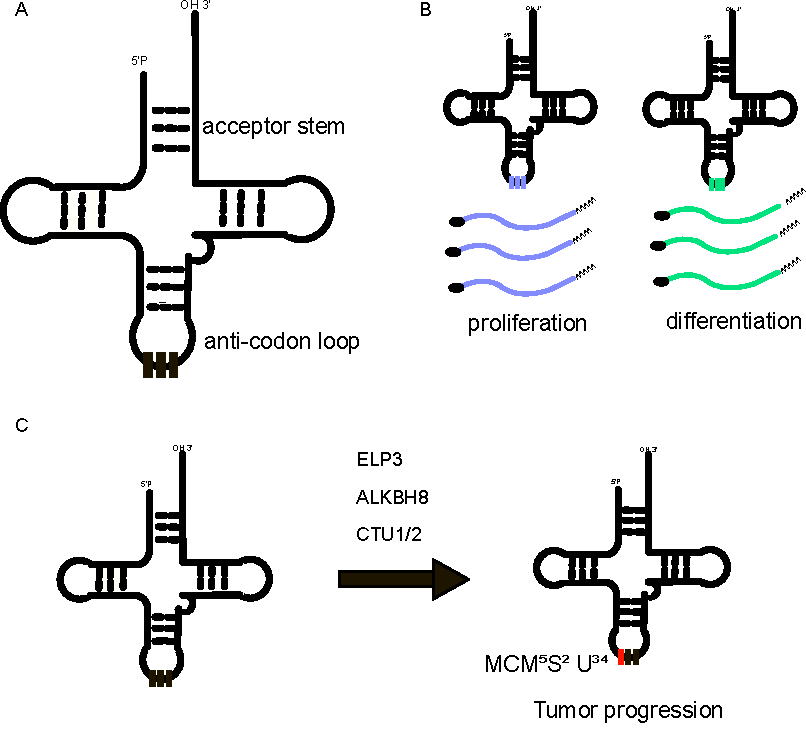
\includegraphics{./figures/tRNA.pdf}
  \caption{ Schematic representations of (A) the tRNA cloverleaf structure with indicated anti-codon and amino acid acceptor sites;  (B)  the proliferation and differentiation mRNAs dependent on distinct tRNA subsets; (C) the U34 wobble position and the catalytic enzymes involved in this modification that is implied in tumor progression.
 \label{fig:tRNA}}
\end{wrapfigure}

As touched upon earlier, tRNAs are an essential part of the translation
machinery that carry the amino acids to the ribosome. In eukaryotes,
tRNAs consist of a 76-90 long nucleotide sequence set into a
``cloverleaf'' structure forming several loops (Sharp, Schaack, Cooley,
Burke, \& Soil, 1985) (\textbf{see figure \ref{tRNA}}). The acceptor
stem binds the amino acid carried by the tRNA, while the anti-codon loop
binds to the mRNA within the ribosome via classical watson-crick pairing
(Watson \& Crick, 1953). Multiple codons can encode for the same amino
acid (synonymous codons), however the availability of the tRNAs for
different codons may vary which can influence elongation rates and thus
protein synthesis.

This supply ( i.e.~tRNA availability) and demand (i.e.~codon
composition) relationship has been found to vary across different
cellular states, e.g.~proliferation and differentiation. Gingold et. al.
observed two differen tRNA subsets; one induced under proliferation that
is otherwise repressed and a subset with similar regulation under
differentiation of which the supply matches the codon demand of the
transcriptome (Gingold et al., 2014). This model has been disputed and
it was proposed that the observed differences would be attributed to GC
content in the mRNA (Rudolph et al., 2016). Nevertheless, abbarent tRNA
expression and codon usage have been reported in cancer (Z. Zhang et
al., 2018). Furthermore, a comprehensive study including small RNAseq
(i.e.~for identification of tRNAs) and protein samples across 17 tissues
obtained from the The Cancer Genome Atlas (TCGA) reported a tRNA
signature stratified by Ki67 (a proliferation marker) staining with
implications for patient survival (Hernandez-Alias, Benisty, Schaefer,
\& Serrano, 2020). Therefore, while a consensus on proliferation
specific tRNA subsets might not have been reached, emerging evidence
implicates a role thereof in cancer (Gingold et al., 2014;
Hernandez-Alias et al., 2020; Z. Zhang et al., 2018). For instance,
increased expression of \(tRNA_{CCG}^{Arg}\) and \(tRNA_{UUC}^{Glu}\)
has been observed in breast cancer cell lines and proposed to drive
metastasis (Goodarzi et al., 2016).

Others report of a role of tRNAs in cancer attributed to tRNA
modifications, specifically at the U34 anti- codon (or wobble) position
which is highly conserved (El Yacoubi, Bailly, \& de Crécy-Lagard, 2012;
Rapino, Delaunay, Zhou, Chariot, \& Close, 2017). The ability to Wobble
was proposed by Francis Crick and refers to the ability of
non-Watson-Crick base pairing of tRNA anti-codons (F. H. Crick, 1966).
This enables a smaller set of tRNAs (41-55 in eukaryotes) to encode for
the 64 possible codon combinations (Goodenbour \& Pan, 2006). In
mammals, the U34 modification catalytic cascade involves the
acetyltransferase Elongator (ELP3), the methyltransferase TRM9-like
domain of Alkylation repair homolog 8 (ALKBH8), and the urmylation (URM)
pathway, that includes the cytosolic thiouridylase homolog 1 and 2
(CTU1/CTU2) (Kalhor \& Clarke, 2003; Karlsborn et al., 2014). These
enzymes ultimately modify the U34 modification into
5-methoxycarbonyl-methyl-2-thiouridine (\(mcm^5s^2U\)) which ensures
cognate codon recognition. This modification is thought to occur in
tRNAs with a U in the wobble position, e.g. \(tRNA^{UUU}\),
\(tRNA^{UUC}\), \(tRNA^{UUG}\), \(tRNA^{UCC}\), and \(tRNA^{UCU}\).

Loss of the ability to modify U34 has been shown to reduce translation
elongation rates with varying effects on protein expression (Deng et
al., 2015; Nedialkova \& Leidel, 2015; Zinshteyn \& Gilbert, 2013).
While in some cases U34 dependent signalling led to ribosome stalling
resulting in protein aggregates and increased stress (Nedialkova \&
Leidel, 2015; Zinshteyn \& Gilbert, 2013), others reported a subtle
dowregulation of proteins encoded by mRNAs requiring U34-modified tRNAs
(Deng et al., 2015). U34 modification dependent tRNAs have been shown to
play a role in cancer. For example, ELP3 is important in tumor
initiation in intestinal epithelia and promotes breast cancer invasion
as well as progression to metastasis (Delaunay et al., 2016; Ladang et
al., 2015).

\subsection{RNA binding proteins and trans-acting factors}

The UTRs of an mRNA contain sequence elements to which small RNA and RNA
binding proteins (RBPs) bind and exert translational regulation.
\subsubsection{miRNAs} For instance, microRNAs (miRNA), a small class of
non-coding RNA. The precise role and mechanisms in regulation of
translation of miRNAs is still under active investigation (Oliveto,
Mancino, Manfrini, \& Biffo, 2017). However, they can directly bind to
other mRNAs and silence them accomplished through translational
repression or destabilisation {[}Jonas2015{]}. Regulation of gene
expression by miRNAs has been observed in cancer where miRNAs have been
implicated to promote tumorgenesis or act as tumor suppressors
(Muniyappa et al., 2009; Nagpal et al., 2015; Sampson et al., 2007; Tian
et al., 2010). \subsubsection{RNA binding proteins} RBPs are a class of
proteins involved in many regulatory steps of gene expression and
account for \textasciitilde{}7.5\% of the protein coding genes. RBPs
bind to elements in the 3' UTRs, e.g.~the poly-a tail. The
poly-A-binding-protein (PABP) is a RBP involved in mRNA translation
initiation. PABP is thought to form a closed loop complex of the 3' end
to the 5' by interacting with eIF4G. This closed loop is proposed to
promote translation and prevent mRNA decay (Afonina, Myasnikov,
Shirokov, Klaholz, \& Spirin, 2014; Amrani, Ghosh, Mangus, \& Jacobson,
2008) (\textbf{see also figure \ref{fig:initiation}}).

Another site is the U-rich cytoplasmic polyadenylation site (CPE) to
which cytoplasmic polyadenylation element binding proteins (CPEBs) can
bind (\emph{see Figure \ref{fig:UTRFeat}}). Studies in \emph{Xenopus}
oocytes indicate that CPEB associates with a non-canonical poly(A)
polymerase (Gld2) and a poly(A) deadynelase (PARN). PARN has a higher
activity than Gld-2 and thus leads to shortening of the Poly(A) tail
(Barnard, Ryan, Manley, \& Richter, 2004). However, hormonal stimulation
leading to CPEB phophorylation removes PARN from the complex thereby
promoting poly(A) tail elongation through Gld-2 (J. H. Kim \& Richter,
2006). Furthermore, in \emph{Xenopus} oocytes, CPEB associated with an
eIF4E binding protein maskin. Maskin bound to eIF4E prevents eIF4F
complex formation which represses mRNA translation (Ivshina, Lasko, \&
Richter, 2014; Stebbins-Boaz, Cao, de Moor, Mendez, \& Richter, 1999).
Therfore, CPEBs can regulate translation by altering 3' UTR lengths and
are involed in transaltional repression by blocking eIF4A association
with the 5' cap in \emph{Xenopus} oocytes. While the role of CPEB
mediated regulation has been decribed mostly in \emph{Xenopus} oocytes,
dysregulation of CPEBs has been described in glioblastoma, colorectal
and pancreatic cancer (Y.-T. Chang et al., 2014; Ortiz-Zapater et al.,
2011; Villanueva et al., 2017).

Another important RBP implicated in regulation of translation is Human
antigen R (HuR). HuR preferentially binds to AU-rich sequences in the 3'
UTR and acts as a stabilizing agent and is involved in RNA-processing
(Baou, Norton, \& Murphy, 2011; X. C. Fan \& Steitz, 1998; T. D. Levine,
Gao, King, Andrews, \& Keene, 1993; S. S.-Y. Peng, Chen, Xu, \& Shyu,
1998). In RKO colorectal carcinoma cells HuR has been shown to enhance
protein synthesis of p53 after exposure to short-wavelength UV light
(UVC) by binding the 3' UTR (Mazan-Mamczarz et al., 2003). The enhanced
effect on protein synthesis was not mediated by stability as HuR failed
to stabilise p53 upon UVC exposure. In U2O cells, overexpression of HuR
led to a dose dependent increase in eIF4E protein levels. The increase
in protein levels was atrributed to eIF4E transcript stabilisation
through binding of HuR to AU-rich elements (AREs) in the 3' UTR of eIF4E
(Topisirovic et al., 2009). Other known drivers of tumor progression
that are targetted by HuR include hypoxia inducible factor 1 (HIF-1),
VEGF, c-Myc (Denkert et al., 2004; López de Silanes et al., 2003; López
de Silanes, Lal, \& Gorospe, 2005). Furthermore, studies in breast,
colon and lung cancer observed correlation between HuR and malignancy
(Denkert et al., 2004; López de Silanes et al., 2003, 2005).

\clearpage
\section{Expertimental methods to measure mRNA translation} \label{exptMethod}

\begin{wrapfigure}{r}{0.6\textwidth}
    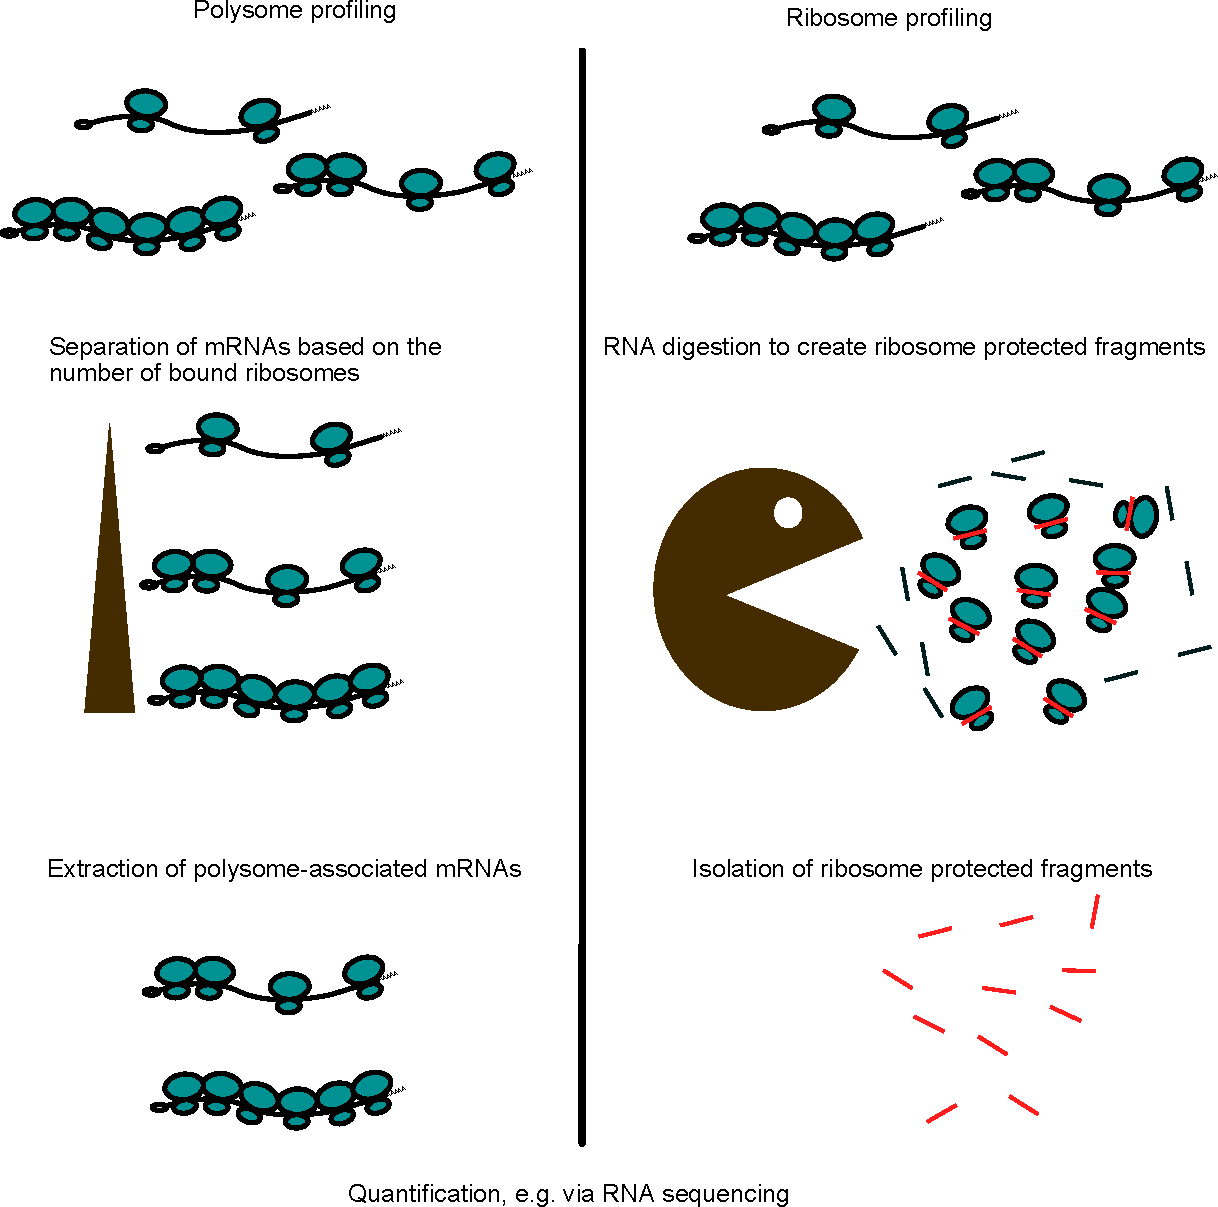
\includegraphics{./figures/polyRibo.pdf}
  \caption{Polysome profiling and ribosome profiling workflows. In polysome profiling a fraction from whole cytoplasmic RNA is loaded onto a sucrose gradient on which they get separated by sedimentation using ultra centrifugation. Fractions corresponding to efficiently translated mRNAs are collected and can be quantified with for example RNA sequencing (left). During ribosome profiling a fraction from the whole cytoplasmic RNA is exposed to a digestion agent which disturbs the RNA. The ribosomes will protect fragments thereby creating ribosome protected fragments. These fragments are then isolated and can be sequenced.  \label{fig:polyRibo}}
\end{wrapfigure}

Two methods are predominantly used for measuring mRNA translation, or
changes in translation efficiencies across conditions, namely polysome
profiling and ribosome profiling (\textbf{see figure
\ref{fig:polyRibo}}). These methods measure mRNA translation by
capturing the number of ribosomes an mRNA is associated with. The number
of bound ribosomes is an adequate estimator changes in translation
efficiencies when initation is rate limiting. This assumption is
supported by findings using polysome profiling in yeast cultured in
nutrient rich medium where initiation was rate-limiting for most mRNAs
(Arava et al., 2003). Furthermore, a recent ribosome profiling study
assessed transcriptome-wide elongation rates. This revealed a similar
rate of elongation for mRNAs of different classes, i.e.~mRNAs that
differed in their 5' UTRs or codon composition (Ingolia et al., 2011).

\subsection{Polysome profiling}

Polysome profiling is a technique to measure changes in translational
efficiencies of mRNAs between two or more conditions. Polysome profiling
allows for separation of polysomes from monosomes, ribosomal subunits
and messenger ribonucleoprotein particles (mRNPs). During the assay,
ribosomes are immobilized on the mRNAs using translation elongation
inhibitors (e.g.~cycloheximide (CHX)). A portion of cytoplasmic RNA
extracts then sediment on a linear sucrose gradient (5-50\%) using ultra
centrifugation. The resulting gradient is fractionated and mRNAs with
different number of bound ribosomes can be extracted and analyzed for
changes in translational efficiency (Gandin et al., 2014). Typically
fractions belonging to mRNAs with more than 3 bound ribosomes are
pooled. A 3-ribosome cut off has been chosen as it is thought to capture
most biologically relevant changes in translation efficiency (Gandin et
al., 2016b).

\begin{wrapfigure}{r}{0.6\textwidth}
    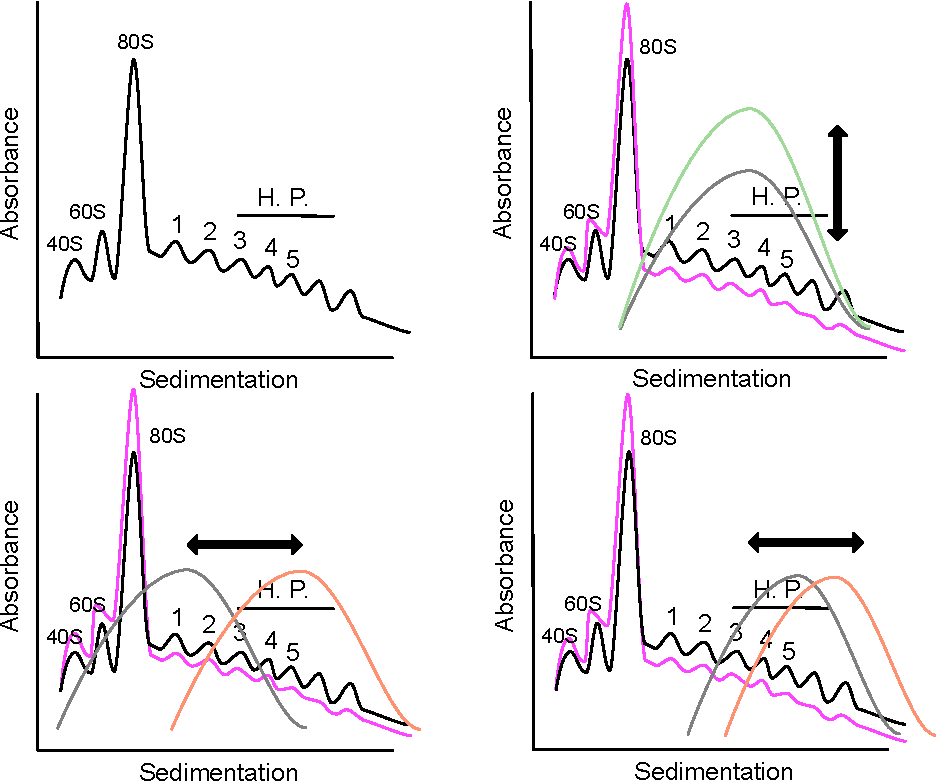
\includegraphics[width=0.9\linewidth]{./figures/polysome_shifts.pdf}
  \caption{Polysome profliles -  (top left) Schematic representation of a polysome profile using linear sucrose gradient fractionation. Indicated in the polysome profiles are the 40S, 60S ribosomal subunits as well as the 80S monosome. H.P. indicates heavy polysome fractions.Between conditions (i.e. black an pink lines) distribution changes for mRNA abundance (grey and green; top right), translation (grey and red; bottom left) and translation within high polysome fractions (grey and red; bottom right) are illustrated. \label{fig:polysome}}
\end{wrapfigure}

An illustration of a polysome profile with peaks for the 40S, 60S
subunits and 80S ribosome can be seen in (\textbf{Fig \ref{fig:polysome}
top left}). Subsequent peaks along the frations indicate the mRNAs with
2 or more bound ribosomes. mRNAs are typically normally distributed
along the fractions, i.e.~in a pool of the same mRNA many will be
associated with different numbers of ribosomes (Gandin et al., 2016b).
Changes in mRNA abundance may lead to an overall increase in the amount
of isolated polysome-associated mRNA without a shift of the distribution
along the fractions (\textbf{Fig \ref{fig:polysome} top right}). This
means that the translation efficiency per mRNA remains unchanged.
Changes in translational efficiency can be observed by shifts of
polysome association for mRNAs from the light (inefficiently translated)
towards the heavy (efficiently translated) polysome fractions or vice
versa in the absence of changes in total mRNA levels(\textbf{Fig
\ref{fig:polysome} bottom left}). Shift within the heavy polysome
fractions (i.e.~with a mean distribution around 4 bound ribosomes to 7
bound ribosomes) can also occur (\textbf{Fig \ref{fig:polysome} bottom
right}). Quantification of mRNA levels within each fraction can be
assessed using Northern blotting or reverse transcription quantitative
polymerase chain reaction (RT-qPCR). For transcriptome wide studies
quantification is done using either DNA-microarrays or RNA sequencing.

Pooling of mRNAs as well as collection of multiple fractions makes
polysome profiling inconvenient when dealing with large samples sizes or
experiments with low amounts of input RNA. Therefore, an optimized
sucrose gradient was developed where mRNAs bound to \textgreater{}3
ribosomes are collected on a sucrose cushion and thereby can be isolated
from one single fraction (Liang et al., 2018). This optimized gradient
allows for application of polysome profiling in small tissue samples
where RNA quantity is limiting and reduces labor intensity of the assay.

Polysome-associated mRNA levels are subject to changes in translation
efficiency as well as factors contributing to cytosolic mRNA levels that
impact to pool of mRNAs that can associate with ribosomes
e.g.~transcription and mRNA stability. Therefore, to identify true
changes in translation efficiency it is important to collect cytoplasmic
mRNA and polysome-associated mRNA from the same sample in parallel to
correct for such mechanisms during downstream analysis.

\subsection{Ribosome profiling} \label{riboseq}

For R17 bacteriophage ribosome protected RNA fragments (RPFs) have been
obtained in the 1960s ribonucleosases to trim away mRNA sequences not
protected by ribosomes (J. A. Steitz, 1969). More recently ribosome
profiling has been developed. Ribosome profling enables sequencing of
RPFs on a transcriptome-wide scale (Ingolia, 2016; Ingolia,
Ghaemmaghami, Newman, \& Weissman, 2009). In the assay ribosomes are
immobilized on the mRNAs using, similar to polysome profiling,
translation elongations inhibitors (e.g.~CHX).

RPFs are obtained by RNAse treatment that degrades the links of RNA
between ribosomes leaving single ribosomes with a \textasciitilde{}28
nucleotide long RNA fragment within each ribosome. However, as ribosomal
RNAs (rRNA) is also degraded during this process they represent a big
fraction herein. The RPFs are then isolated using ultra centrifugation
through a sucrose cushion. During this step other RNA fragments such as
rRNAs, non-coding RNAs (ncRNAs) or large ribonucleoprotein complexes can
co-migrate and contaminate the sample. Typically RPFs with a size
ranging from 25-30 nucleotides are selected for quantification. However,
among these sizes could be RNA protected by RBPs that have no ribosome
associated to it. Furthermore, ribosomes undergoing conformational
changes have been shown to protect fragments corresponding to a length
of 21nt only when translation elongation is blocked by e.g.~CHX (L. F.
Lareau, Hite, Hogan, \& Brown, 2014). Therefore, size selection can
distort the estimation of translation efficiency from ribosome profiling
data (Dmitry E. Andreev et al., 2017). From the resulting RPFs libraries
can be constructed and quantified using RNA sequencing. During library
construction additional biases due to enzyme sequence preferences can be
introduced that can lead wrong estimations of codon positions within the
ribosome (Artieri \& Fraser, 2014a).

Recently, Ribo-seq Unit Step Transformation (RUST) has been developed
(O'Connor, Andreev, \& Baranov, 2016). This algorithm can reveal mRNA
sequence features affecting RPF density globally. The authors applied
RUST to 30 publicly available data sets and identified substanial
sequence heterogeneity affecting RPF densities. Thus, sequence bias is
prominent in ribosome profiling data (O'Connor et al., 2016).

Initially, fragmented total mRNA using alkaline hydrolysis of the same
size were retrieved in paralell to RPFs. This was achieved by extraction
of total mRNA from cell lysate followed by purification via recovery of
polyadenylated messages or removal of ribosomal RNA (Brar \& Weissman,
2015; Ingolia et al., 2009). The random fragmentation of total mRNA has
been shown to underlie experimental bias. Therefore, now sequencing of
unfragmented total mRNA is sequenced in parallel is preferred.

\subsection{Comparing ribosome and polysome profiling}

Albeit both methods generate count data after quantification with RNA
sequencing, there are some key aspects that differ between the
techniques. Polysome profiling separates efficiently translated mRNAs
from non- efficiently translated mRNAs along a sucrose gradient thereby
creating an mRNA based perspective for analysing changes in
translational efficiencies. In contrast, ribosome profiling determines
translational efficiencies by counting the number of RPFs of both
efficiently and non-efficiently translated mRNAs. This can have
implications for identifaction of transcript variants. For example If a
ribosome would not protect a fragment spanning a variant the information
would be lost during ribosome profiling (S. N. Floor \& Doudna, 2016).
Whereas in polysome profiling the quantification is based on the whole
mRNA. This gives polysome profiling the advantage in cases where
transcript variants with different 5' UTR lengths are of interest.

Shifts in ribosome association, can be dramatic (i.e.~near complete
dissociation of ribosomes from an mRNA) or subtle (shifts from e.g.~2 to
4 ribosomes) and could be due to different properties of the mRNAs
(Gandin et al., 2016b). When dramatic and subtle changes in ribosome
association are present in parallel, ribosome profiling is biased
towards identification of dramatic shifts and masks the subtle ones
(Gandin et al., 2016b). Gandin et. al. showed under mTOR inhibition
ribosome profiling studies would predominantly identify TOP mRNAs
(i.e.~heavy shifters). Furthermore, polysome profiling also identified
non-TOP mRNAs when mTOR is inhibited (Gandin et al., 2016b). Therefore,
in scenarios where global mRNA translation is affected application of
ribosome profiling could lead to imprecise biological conclusions. The
masking of subtle changes has been attrituted to the indirect estimation
of translation efficiencies from counting RPFs for ribosome profiling,
which is highly dependent on the abundance of mRNAs. In polysome
profiling this effect is much less pronounced as changes in translation
efficiency are directly estimated from the mRNAs associated with heavy
polysomes (Masvidal, Hulea, Furic, Topisirovic, \& Larsson, 2017).
Therefore, polysome profiling is more suitable in studies that aim to
analyse global changes in translation efficiences. (Gandin et al.,
2016b; Masvidal et al., 2017).

An advantage of ribosome profiling is that it provides exact nucleotide
positions occupied by ribosomes. This offers information at a single
nucleotide level where the ribosome is located at the mRNA. Polysome
profiling cannot reveal ribosome locations along the mRNA. The single
nucleotide resolution of ribosome profiling is necessary in contexts
studying events such as ribosomal frame shifts (Rato, Amirova, Bates,
Stansfield, \& Wallace, 2011) or uORF translation (Dmitry E Andreev et
al., 2015). One limitation of ribosome profiling to identify features
such as uORFs is the use of elongation inhibitors in the protocol,
e.g.~CHX. After CHX treatment elongation is not immediatly inhibited but
continues for several cycles (Hussmann, Patchett, Johnson, Sawyer, \&
Press, 2015). Studies investigating stress in yeast showed that CHX
increase in ribosome occupancy was due to CHX treatment rather than
stress (Gerashchenko \& Gladyshev, 2014). Therefore, CHX treatment can
introduce biases in ribosome profiling obscuring potential sequence
features important for translational regulation (@ Gerashchenko \&
Gladyshev, 2014; Hussmann et al., 2015).

Both methods have their strengths and weaknesses and therefore each
method should be considered depending on the underlying biological
question. \newline
\section{Modes for regulation of gene expression through mRNA translation} \label{modes}

\begin{wrapfigure}{r}{0.6\textwidth}
  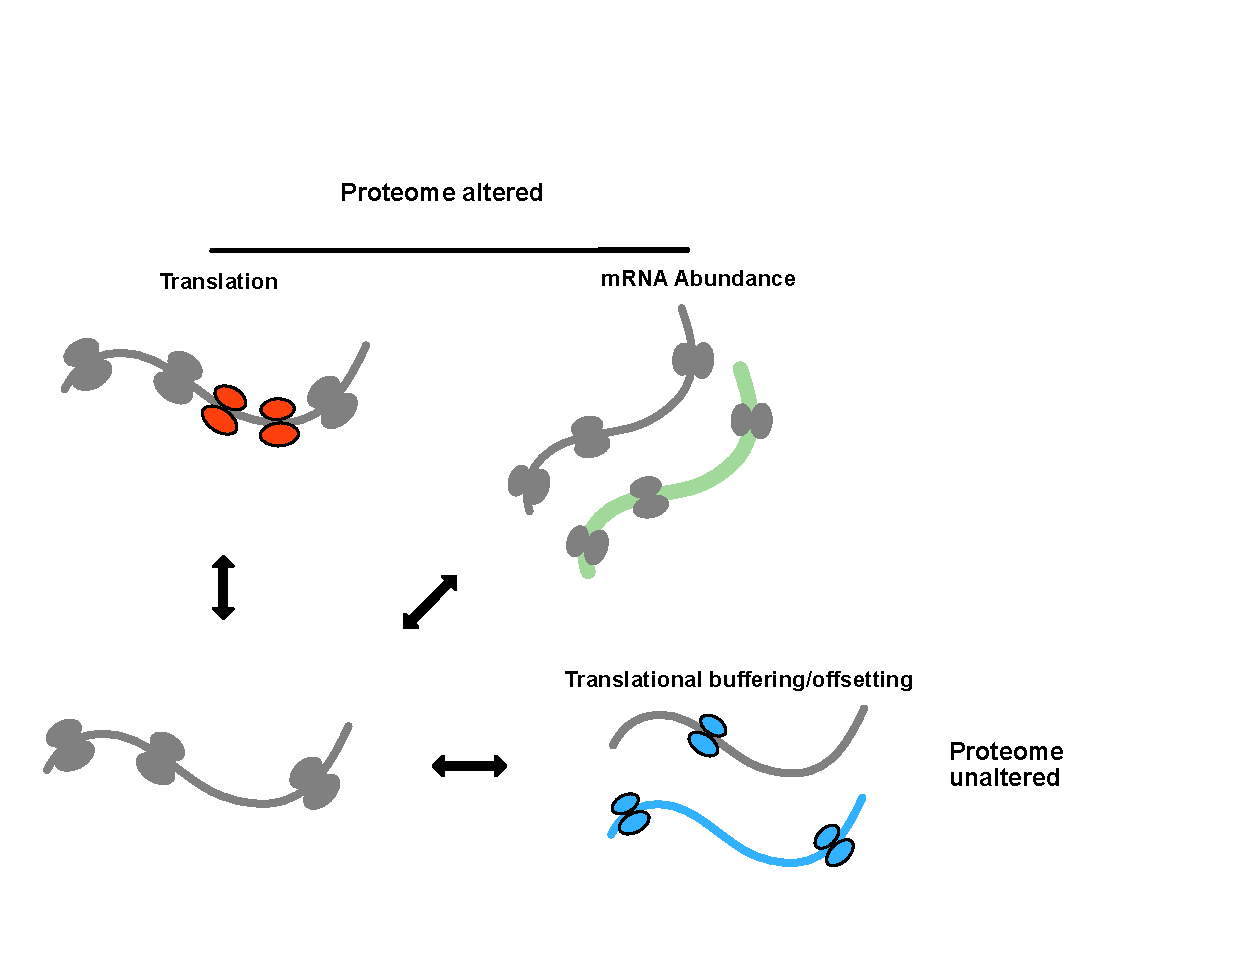
\includegraphics{./figures/geneModes_MRNA.pdf}
  \caption{Regulatory modes of gene expression - Schematic representation of regulatory modes of translation efficiency in a fold-change scatter plot. Indicated in red are changes in translation (i.e. changes in translated mRNA but not total mRNA), in green changes in mRNA abundance (i.e. congruent changes between total mRNA and translated mRNA) and in blue translational buffering (i.e. changes in total mRNA levels but not translated mRNA levels). TE changes as the TE-score would estimate them are indicated.\label{fig:modes}}
\end{wrapfigure}

From transcriptome-wide assessments of translation using ribosome or
polysome profiling expression levels are obtained for both cytoplasmic
and polysome-associated mRNAs (or RPFs). For simplicity, from now on,
these RNA types will be referred to as total mRNA (i.e.~cytoplasmic
mRNA) and translated mRNA (i.e.~polysome-associated mRNA or RPFs). The
estimation of expression levels for both translated mRNA and total mRNA
allows for interrogation at two steps of the gene expression pathway and
their interaction. The interplay of total mRNA with translated mRNA can
give valuable insights about the underlying mechanisms that govern gene
expression in the studied system.

When comparing perturbed systems to their corresponding control state
three ``modes'' in which translated mRNA and total mRNA distinctly
interact can be observed (\emph{See figure \ref{modes}}). We refer to
these modes as ``mRNA abundance'', ``translation'' (i.e.~changes in
translation efficiencies leading to altered protein levels) and,
``translational buffering'' (i.e.~changes in translation efficiencies
ensuring protein homeostasis).

\subsection{mRNA Abundance}

A change in mRNA abundance is observed when the translated mRNA level
changes to a similar magnitude as the total mRNA level. For these mRNAs
the translation efficiency is unaltered, as the change in total mRNA
levels explains the change in translated mRNA levels. This is in line
with the model of ``weak'' and ``strong'' mRNAs where the abundance of
mRNAs alters the ability to compete for translation initiation factors.
The underlying biological implication for this mode mRNAs is often
related to transcription or mRNA stability (\emph{See figure
\ref{modes}}). While genes of the mRNA abundance mode do not change
their translation efficiency, the change in overall translation is
expected to reshape the proteome.

\subsection{Translation}

A change in translation occurs when translated mRNA levels either
increase or decrease, while corresponding total mRNA levels remain
constant or change to a lesser extent. The change in ribosome
association indepedent of total mRNA levels is therefore a change in
their translation efficiency. A prominent example of this mode can be
observed for TOP mRNAs. Under conditions when mTOR is inhibited, TOP
mRNAs show a near complete dissassociation from ribosomes (Gandin et
al., 2016a). Furthermore, during the ISR, translation of ATF4 is altered
due to eIF2\(\alpha\) phosphrolaytion. mRNAs under the translation mode
are expected to reshape the proteome (\emph{See figure \ref{modes}}).

\subsection{Translational buffering} \label{modeBuffering}

The third mode of regulation of gene expression is termed translational
buffering. Under this mode, a change in total mRNA levels is observed,
whereas polysome-associated mRNA levels remain constant between
conditions. Translational buffering also reflects a change in
translation efficiency as the proportion of mRNAs to associated with
ribosomes is altered. Yet, the change in translation efficiency upon
translational buffering (i.e.~ribosome associated is unaltered) is
distinct to that from changes in translation where ribosome association
is explicitly modulated. In contrast to changes in translation and mRNA
abundance, translational buffering has been shown to maintain protein
homeostasis rather than reshape the proteome (\emph{See figure
\ref{modes}}) (Lalanne et al., 2018; Lorent et al., 2019; McManus, May,
Spealman, \& Shteyman, 2014).

Currently the literature supports multiple forms of translational
buffering. Translational buffering can compensate for differences in
mRNA levels due to e.g.~differences in gene dosages, so that protein
levels remain similar (Dassi et al., 2015; Lalanne et al., 2018).
Furthermore, rather than compensating it can ``offset'' modulations of
total mRNA levels at the level of translation to temporarily alter the
mRNA:protein ratio (Lorent et al., 2019).

Translational buffering in its compensation form has been observed at
steady state levels. A study comparing co-evolution of transcription and
translation across seven different organs and mammals showed overall
greater divergence of transcription as compared to translation (Z.-Y.
Wang et al., 2020). Similar compensation at the level of translation has
been observed between individuals, tissues and prokaryotes (Artieri \&
Fraser, 2014b; C. Cenik et al., 2015; Dassi et al., 2015; Lalanne et
al., 2018; Perl et al., 2017).

Compensation via translational buffering can also enforce equilibration
of pathway or protein complex stoichometry (Lalanne et al., 2018; Li,
Burkhardt, Gross, \& Weissman, 2014). An example of this was observed in
evolutionary distant bacetria, i.e.~B. subtilis and E. coli. In B.
subtilis translation related factors rpsP and rplS are located in
different operons, whereas in E. coli they lie within an operon together
with rimM and trmD. While B. subtilis can fine tune transcription at the
different operons, in E. coli these will be transcribed together.
However, rimM and trmD are only needed in low protein abundance, whereas
rpsP and rplS are required in high abundance. E. coli compensates the
transcriptional input at the translational level and thus equilibriates
for requirements in pathway stoichometry (Lalanne et al., 2018).

As mentioned above, a different form of translational buffering can be
observed in perturbed systems that offset changes in total mRNA levels
at the level of translation temporarily. For example, translational
offsetting was observed in prostate cancer cells where a transcriptional
program was induced under estrogen receptor \(\alpha\) (ER\(\alpha\))
depletion that showed no increase in polysome-associated mRNA. mRNAs
whose transcription was translationally offset required the tRNA u34
modification. ER\(\alpha\) has been shown to regulate the expression of
the catalytic enzymes required for the u34 modification (Lorent et al.,
2019). Thus, depletion of ER\(\alpha\) led to that tRNAs could not be
properly modified at the U34 position and therefore the translation
efficiency of mRNAs requiring the modification was reduced despite
increased total mRNA levels. \newline
\section{Algorithms for analysis of changes in translation efficiencies}\label{algorithm}

As discussed above, mRNA translation can reshape the proteome via
multiple modes for regulation of gene expression. These modes can have
different underlying biological mechanisms. It is therefore warrented to
distinguish these them in analysis of translation efficienies. In this
section we will discuss methods to analyse polysome-profiling and
ribosome profiling data to estimate changes in translation efficiencies
across 2 or more conditions and how these methods identify different
modes of gene expression.

Initially analysis of transcriptome-wide translation studies used an
approach called the translation efficiency score (TE-score) that uses
the following equation:
\[\varDelta TE = \frac{\frac{P_{c2}}{T_{c2}}} {\frac{P_{c1}}{T_{c1}}}\\\]

This score is calculated the ratio of the ratios between
polysome-associated mRNA levels (P) divided by total mRNA levels (T)
within each condition (i.e.~C1 and C2). The TE- score approach has been
shown to be prone to spurious correlations (Larsson, Sonenberg, \&
Nadon, 2010). Spurious correlations arise due to that the ratio of
polysome-associated mRNA and total mRNA can systematically correlate
with total mRNA levels which is not corrected for in this equation and
leads to an elevated type-1 error.

\textbf{Figure \ref{fig:TE}} gives an overview of the relationship
between a change in TE-score and each gene expression mode (\textbf{see
also figure \ref{fig:modes}}). Changes in mRNA abundance will lead to a
\(\varDelta\)TE close to 0 in log space (i.e.~no change in translation
efficiency) as total mRNA and translated mRNA change with a similar
magnitude. However, in the case of both translation and translational
buffering, the nominator and denominator in the TE-score equation change
leading to a \(\varDelta\)TE (TE \textless{} 0 or TE \textgreater{} 0)
and thereby identification of both changes in translation and
translational buffering simultaneously. Therefore, the TE-score method
fails to differentiate between changes in translation and translational
buffering which can have drastic consequences for the biological
interpretation of the results (Oertlin et al., 2019) (\textbf{see also
section \ref{modes}}).

\begin{wrapfigure}{o}{0.5\textwidth}
  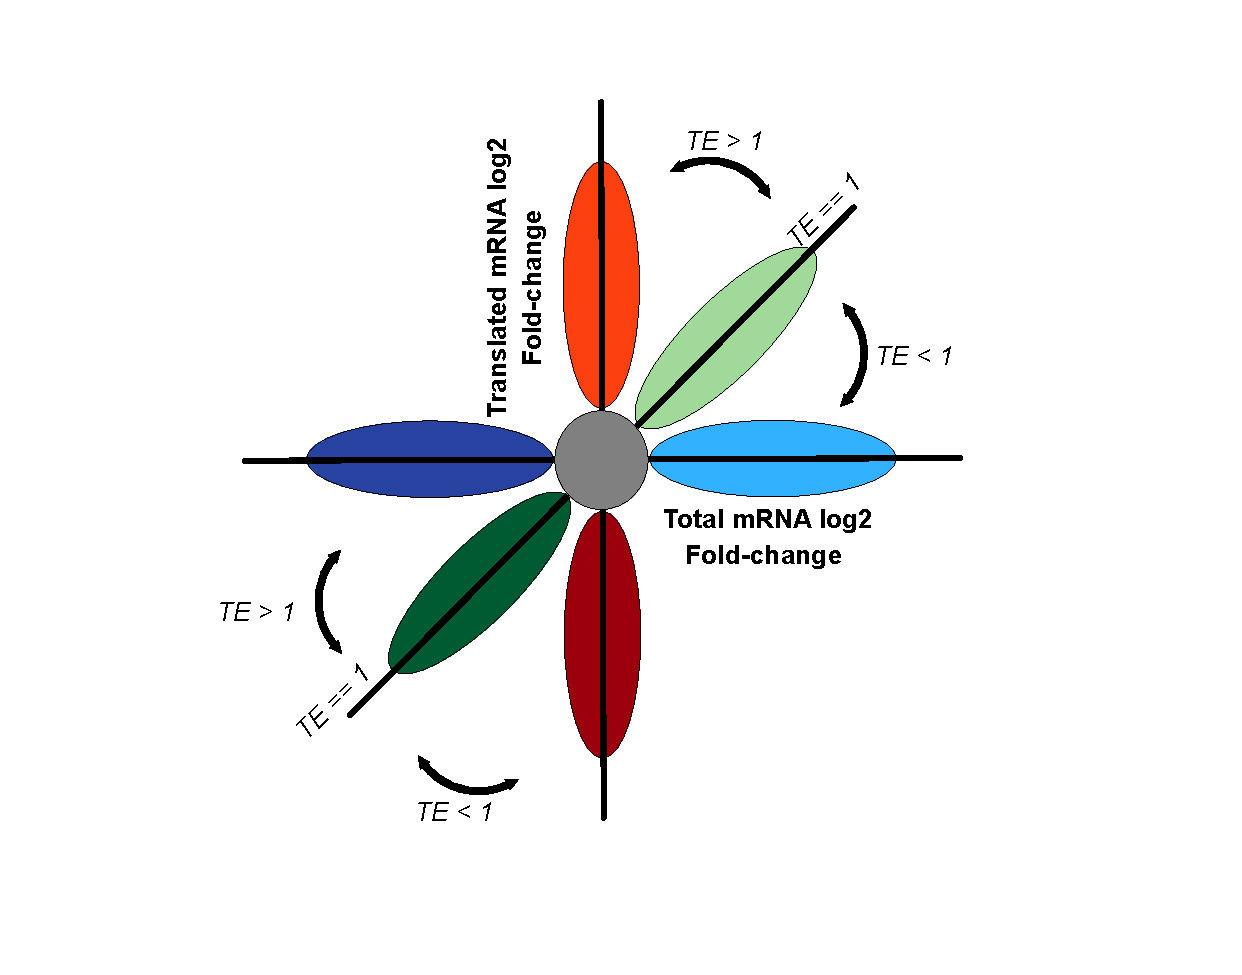
\includegraphics{./figures/geneModes_TE.pdf}
  \caption{TE scores for regulatory modes of gene expression -  Schematic representation of regulatory modes of translation efficiency in a fold-change scatter plot. Indicated in red are changes in translation efficiency altering protein levels, in green changes in mRNA abundance and in blue changes in translation efficiency leading to translational buffering/offsetting. The shifts for the translation efficiency (TE) score are indicated. \label{fig:TE}}
\end{wrapfigure}

The TE-score approach was questioned when proposing the Analysis of
Translation Activity (anota) algorithm which was developed for
DNA-microarray data (Larsson et al., 2010). Anota combines analysis of
partial variance (APV) (Schleifer, Eckholdt, Cohen, \& Keller, 1993)
with a random variance model (RVM) (G. W. Wright \& Simon, 2003). RVM
estimates gene variance using shared information across all genes to
increase power for detection of differential expression (G. W. Wright \&
Simon, 2003). anota uses a two-step process that firstly assesses the
model assumptions for (i) absence of highly influential data points,
(ii) samples classes sharing a common slope, (iii) homoscedasticity of
residuals and (iv) normal distribution of per gene residuals. In the
second step anota performs analysis of changes in translational activity
using the following model:

\[y_{gi} = \beta_g^{RNA}\ X_i^{RNA}+ \beta_g^{cond}\ X_i^{cond} + \varepsilon_{gi}\]

here \(y_{gi}\) is the polysome associated mRNA expression,
\(\beta_g^{RNA}\) describes the relationship to total RNA for the
\(gth\) gene of the \(ith\) sample column of model matrix \(X\);
\(\beta_g^{cond}\) represent the difference in intercept between
treatment classes and \(\varepsilon_{gi}\) denotes the residual error.
\clearpage

\begin{wrapfigure}{o}{0.5\textwidth}
  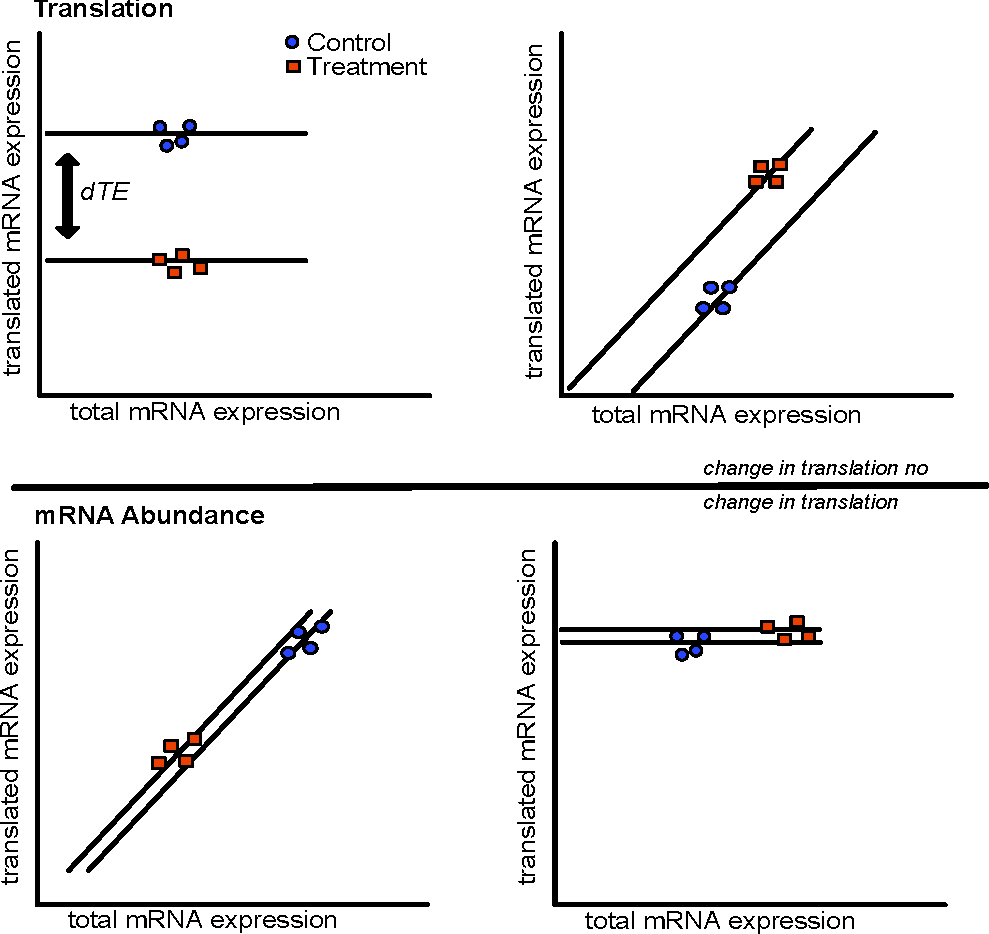
\includegraphics{./figures/geneModes_anota_Larsson.pdf}
  \caption{anota gene models - Schematic representation of the anota analysis models. Translation mRNA expression is set out against total mRNA expression for each biological replicate and treatment condition. Top left shows the model of a gene that is deferentially translated (i.e. change in translated but not total mRNA). The difference in the slope intercepts are used to estimate changes in translation efficiencies between conditions i.e. dTE. Other gene models are shown; change in translation efficiency with varying total mRNA levels (top right); change in mRNA abundance (bottom left) and translational buffering (bottom right).
  \label{fig:anota}}
\end{wrapfigure}

Within anota a common slope for the treatment classes that describes the
translated mRNA to total mRNA relationship is calculated. The difference
between the slope intercepts is then interpreted as the change in
translation efficiency. A simplified view of this model is provided in
(\textbf{Figure \ref{fig:anota} top left}). Here expression for
translated mRNA and total mRNA are modeled over two sample classes with
each 4 replicates. Furthermore, changes in translation efficiencies can
also be observed when translated mRNAs shift to a larger extent than the
total mRNA levels (\textbf{Figure \ref{fig:anota} top right}).
Identification of genes in this category can be a challenge, especially
in highly variable data sets, as they resemble mRNA abundance genes
(\textbf{Figure \ref{fig:anota} bottom left}). Nevertheless, using the
linear regression analysis anota accurately corrects changes in
translated mRNA as can be seen in (\textbf{Figure \ref{fig:anota} bottom
right}) where a change in total mRNA but not translated mRNA levels is
observed. For this gene the difference in slope intercepts between
sample classes is small and will not be identified as differentially
translated as would be the case in the TE-score approach. Anota was
developed at a time where translational buffering was not considered in
data sets. Naturally, the method lacks a setting to analyse
translational buffering. This was addressed in anota's successor,
anota2seq, and will be discussed in \textbf{Study 1}.

Advances in experimental methods warrant for appropriate statistical
approaches to analyse data resulting from them. DNA-microarray was the
dominant platform to assess transcriptome-wide changes before the advent
of RNA sequencing. DNA-microarrays measure intensity after hybridisation
events is an indicator of expression, whereas in RNA sequencing reads of
constructed libraries are counted. Intensity data from DNA-microarray
can be normalised and transformed (i.e.~log transformation) to fulfill
the requirements for application of linear models, whereas RNA
sequencing harbours additional characteristics that need to be accounted
for. Therefore, algorithms developed for analysis of DNA- microarray are
not directly applicable to RNA sequencing data as is the case for the
anota algorithm.

RNA sequencing data shows variance that is greater than the mean which
is commonly referred to as overdispersion. Count data from RNA
sequencing have been initially approached using Poisson distributions
which assumes that the variance is equal to the mean (J. Lu et al.,
2005). Now established RNA sequencing analysis frameworks such as edgeR
and DESeq2 use negative binomial distributions in combination with
generalised linear models (GLMs) (Love, Huber, \& Anders, 2014;
Robinson, McCarthy, \& Smyth, 2010). The negative binomial distribution
uses a dispersion parameter to account for differences in the
mean-variance relationship across the expression range (McCarthy, Chen,
\& Smyth, 2012). While analysis principles of DESeq2 and edgeR are
similar they differ in their normalisation method, dispersion estimation
and information sharing across genes. In a simple differential
expression analysis between two conditions with one RNA type the GLM
model would be as in the following equation:

\[log(y_{gi}) = \beta_g^{cond}\ X_i^{cond} + \varepsilon_{gi}\]

here \(\beta_g^{cond}\ X_i^{cond}\) represent the condition
(i.e.~control and treatment) log2 fold change for the \(gth\) gene
\(ith\) sample column of the model matrix X and \(\varepsilon_{gi}\)
denotes the residual error. When analysing changes in translation
effiencies additional parameter for RNA type (i.e.~total mRNA or
translated mRNA) and the interaction between the RNA type and condition
are added so that:

\[log(y_{gi}) = \beta_g^{RNA}\ X_i^{RNA}+ \beta_g^{cond}\ X_i^{cond} + \beta_g^{RNA:cond}\ X_i^{interaction} + \varepsilon_gi\]

In this model, the interaction term is interpreted as the change in
translation effiencies (Chothani et al., 2019). Other methods
(i.e.~Ribodiff (Zhong et al., 2017), Riborex (W. Li, Wang, Uren,
Penalva, \& Smith, 2017) and deltaTE (Chothani et al., 2019)) borrow
this analysis principle of an GLM with an interaction term by applying
this exact model. A notable difference is that Ribodiff allows
dispersion estimation for translated mRNA and total mRNA separately as
variance differences between the RNA types can be expected due to
varying experimental protocols (Liang et al., 2018; Zhong et al., 2017).
While the flexibility of GLMs allows for complex study designs involving
2 or more treatment conditions, Riborex and Ribodiff limit the study
design to only two conditions. DeltaTE gives their users full
flexibility of the DESeq2 GLM model. Xtail is a method developed for
ribosome profiling that makes use of DESeq2 for RNAseq count
normalisation (Z. Xiao, Zou, Liu, \& Yang, 2016). Their assessment of
differences in translation efficiencies relies on probability matrices
for the ratio of translated mRNA over total mRNA within condition and a
between condition ratio of these ratios. Babel was the first algorithm
designed solely for analysis of differential translation and uses an
error-in-variables regression analysis (A. B. Olshen et al., 2013). The
error-in- variables regression allows accounting for variable total mRNA
levels when assessing changes in translation. Although these methods
have distinct approaches to identify changes in translation
efficiencies, their principle of analysis is similar to comparing a
ratio of ratios (see TE-score equation above). Therefore these methods
suffer from similar issues as the TE-score which will be discussed in
\textbf{Study 1}.

\chapter{Aims of this thesis}

This thesis aims to expand current methodologies for analysis of
translation efficiency data and explore the regulation of gene
expression in cancer.

In \textbf{Study I}, we adapted the ANalysis Of Translation Activity
data (anota) algorithm so that it could be applied to next-generation
sequencing data. Furthermore, we implemented the analysis of
translational buffering a recently described mode for regulation of gene
expression. The resulting algorithm was named anota2seq.

We then applied the anota2seq algorithm to investigate changes in
translation efficiencies in two cancer models:

In \textbf{Study II} we unravelled the effects of eIF4A, an RNA
helicase, inhibition using a synthetic rocaglate CR-1-31-B (CR-31) in
pancreatic ductal adenocarcinoma.

In \textbf{Study III} we explored the effects of insulin on gene
expression in multiple cell lines.

\chapter{Results and discussion}

\section{Study 1 - Generally applicable transcriptome-wide analysis of translation using anota2seq}

Initially changes in translation efficiencies were estimated using the
TE-score approach as outlined in section \ref{algorithm}. However, this
method was being shown to be prone to spurious correlations leading to
elevated false positive identification that can result in false
biological conclusions (Larsson et al., 2010). Spurious correlations,
when using the TE-score, can be attributed the inadequate correction for
changes in total mRNA levels when estimating translation efficiencies
(Larsson et al., 2010; Larsson, Sonenberg, \& Nadon, 2011). The Analysis
of Translation Activity (anota) algorithm facilitates analysis of
translational efficiencies that are corrected for changes in total mRNA
levels (Larsson et al., 2011).

Anota was developed for analysis of transcriptome-wide analysis for data
quantified by DNA- microarrays (Larsson et al., 2010). However, advances
in experimental methodologies lead to the development in RNA sequencing.
RNA sequencing and DNA microarray data have distinct characteristics
that need to be accounted for before analysis (\textbf{see section
\ref{algorithm}}). Therefore, while the statistical framework of anota
had been shown as an adequate approach for analysis of translational
efficiencies for data from DNA microarrays it was not directly
applicable to RNA sequencing data. The is due to the mean variance
relationship, a characteristic of RNA sequencing data. This encompasses
that the counts for lower expressed genes show higher variability than
counts for higher expressed genes even after log transformation. Efforts
have been made to make RNA sequencing data more ``DNA- microarray like''
so that algorithms developed for intensity based microarray data can be
applied to count based RNA sequencing data (Law, Chen, Shi, \& Smyth,
2014; Love et al., 2014). Anota2seq, the algorithm developed in this
study, allows for transformation and normalisation of RNA sequencing
data so that the anota statistical frame work can be applied for
analysis of count data.

Another feature of anota2seq is that it allows for statistical analysis
of translational buffering. The need for the analysis of translational
buffering, or the uncoupling of mRNA levels from translation, has been
noted before anota2seq's development by comparing 20 translatomes and
transcriptomes with different underlying stimuli in mammalian cells
(Tebaldi et al., 2012). The same authors proposed a framework, called
tRanslatome, that combines several methodologies for analysis of
differential transcription and translation efficiencies, including
anota, for a comprehensive analysis of transcription and translation as
well as their underlying mechanisms (Tebaldi, Dassi, Kostoska, Viero, \&
Quattrone, 2014).

\begin{wrapfigure}{o}{0.5\textwidth}
  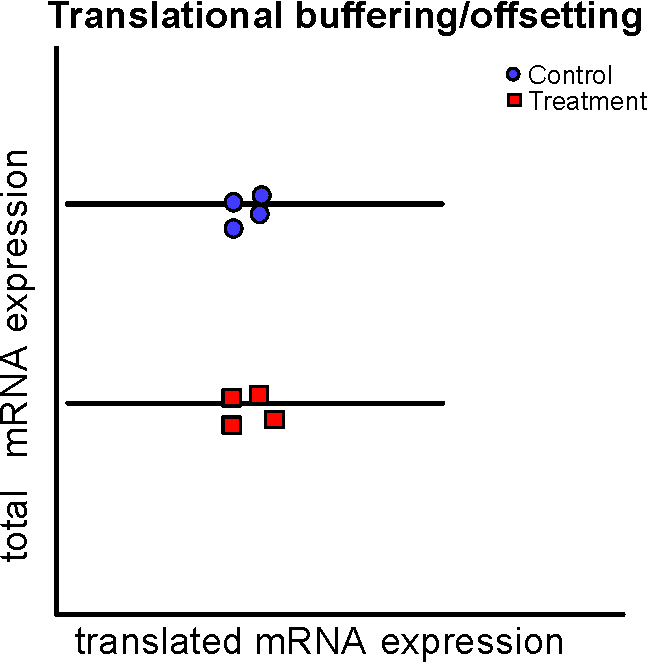
\includegraphics{./figures/geneModes_anota2seq.pdf}
  \caption{anota2seq gene model for analysis of translational buffering /offsetting - Total mRNA expression is set out against translated mRNA expression for each biological replicate and treatment condition. The model shows total mRNA changes that are independent of translated mRNA changes which is classified as translational buffering. It is important to distinguish between the gene modes as their regulation could be due to different underlying biological mechanisms (see section \ref{modes}).
  \label{fig:anota2seq}}
\end{wrapfigure}

Nevertheless, commonly observed in polysome and ribosome profiling data
sets are three gene expression modes, translation, translational
buffering and mRNA abundance. While anota can be used to identify genes
among the translation and mRNA abundance mode, analysis for
translational buffering was not implemented therein (\emph{See Figure
\ref{fig:anota}}). Therefore, one would need to rely on the integration
of several methods to efficiently analyse transcriptome-wide studies of
translation efficiences. Anota2seq addresses this issue by changing the
analysis model as described in section \ref{algorithm} to analyse
changes in total mRNA levels corrected for changes in translated mRNA
levels (i.e.~translational buffering, \textbf{see figure
\ref{fig:anota2seq}}).

Application of anota2seq has successfully identified translational
buffering to which biological mechanisms could be linked, e.g.~as
mentioned earlier translationally bufferring under ER\(\alpha\)
depletion in prostate cancer (\textbf{see section \ref{modeBuffering}})
(Lorent et al., 2019). Furthermore, in \textbf{study 2} translational
buffering can be observed as a compensating mechanisms in ``healthy''
cells upon treatment with an eIF4A inhibitor and in \textbf{study 3} we
identify mTOR dependent translational buffering for mRNAs with certain
3' UTR characteristics.

The aim of this study was to compare anota2seq's performance to other
established algorithms (i.e.~DESeq2, RiboDiff, babel, TE-score and
Xtail) for analysis of translation efficiencies, specifically their
ability to distinguish the three prominent modes of gene expression. To
achieve this we used simulated data. While it is arguable to what extent
conclusion drawn from simulated data can be extended towards empirical
data it allows for a controlled environment where true positive changes
are known in advance. Furthermore, the mean-variance relationship in the
simulated data is based on a real polysome profiling data set to
increase confidence that drawn conclusions are also applicable to
empirical data (Guan et al., 2017). Furthermore, during testing of our
simulation we used an additional data set to estimate parameters from to
generate data sets. Using these simulated data to compare the
performance of the above mentioned algorithms showed almost identical
results.

The simulated data consisted of four replicates for translated mRNA and
total mRNA with a ``control'' and a ``treatment'' condition.
Furthermore, the data sets contained a combination of the following gene
sets:

\emph{``Unchanged''}: For this simulation category we sampled reads from
the same NB distribution for both the control and treatment conditions
in both the translated and total mRNA. This category represents genes
that would be unaffected by e.g.~a stimulus of between cellular states.

\emph{``mRNA abundance''}: For this category the control condition for
both the translated mRNA and total mRNA were sampled from the same NB
distribution. The NB distribution for \textbf{both translated mRNA and
total mRNA} of the treatment condition was altered so that values would
be drawn corresponding to a fold change (negative or positive) ranging
between 1.5 to 3.0. The directionality of the fold changes (i.e.~up or
down regulation) was the same for translated mRNA and total mRNA.

\emph{``translation''}: For this category the control condition for both
the translated mRNA and total mRNA were samled from the same NB
distribution. The NB distribution for \textbf{translated mRNA only} of
the treatment condition was altered so that values would be drawn
corresponding to a fold change (negative or positive) ranging between
1.5 to 3.0.

\emph{``buffering''}: For this category the control condition for both
the translated mRNA and total mRNA were sampled from the same NB
distribution. The NB distribution for \textbf{total mRNA only} of the
treatment condition was altered so that values would be drawn
corresponding to a fold change (negative or positive) ranging between
1.5 to 3.0.

As a first step, we tested whether the methods could properly control
for type-1 errors (i.e.~false positive identification). For this we
simulated a data set with genes belonging only to the ``unchanged''
category. This revealed that babel, but to an even greater extent Xtail,
were unable to control their type-1 error as these methods assigned low
p-values and FDRs when no real changes were present. DESeq2 was
marginally affected by this also. This indicated a limited applicability
of Xtail and babel for statistical analysis of translatomes.

From the comparative analysis of the analysis for changes in translation
efficiencies affecting protein levels we concluded that anota2seq
outperforms all other methods. This was assessed by comparing the area
under the curve from Receiver operating characteristics (ROC) and
precision recall curves. The ROC curves showed a, albeit slightly,
better performance for detecting changes in translation. However, the
precision recall was much higher for anota2seq which can be accredited
to that the analysis principle of the other methods is based on
identifying changes regardless of whether the change is in the
translated mRNA or total mRNA (\emph{as explained in section
\ref{algorithm}}). Nevertheless, when comparing the performance using
simulated data in the absence of genes belonging to the ``buffering''
category anota2seq still showed superior performance.

Next to the a prior knowledge of the introduced changes in the
simulation data, it also allowed us to modify parameters to investigate
the robustness of the methods to increased variance, overall sequencing
depth and differing sequencing depth between samples. Here, all methods
showed robustness against variance and sequencing depth differences
between samples as long as a minimum of 5 million counts per sample was
reached.

A shortcoming in the simulation study is that we did not assess the
effects of systematic batch effects. Batch effects can be introduced
e.g.~during experimental design and there are many methods that try to
correct for these (W. E. Johnson, Li, \& Rabinovic, 2007; Leek, 2014; Y.
Zhang, Parmigiani, \& Johnson, 2020). Other ways to correct for batch
effects is their inclusion in the analysis model, which can be supplied
to the analysis model in DESeq2, edgeR as well as anota2seq. Indeed
analysis of a dataset with prominent batch effects showed that batch
effects can dampen the efficiency of the anota2seq algorithm to identify
changes but can be effectively corrected for in the algorithm.

In this study we developed an analysis algorithm for efficient
transcriptome-wide analysis of translation efficiencies applicable to
DNA-microarrays and RNA seq. Furthermore, anota2seq has been
successfully applied to broaden the knowledge around mRNA translation in
various different contexts (Chan et al., 2019; Chaparro et al., 2020;
Hipolito et al., 2019; Lorent et al., 2019). Furthermore, more recently
anota2seq has been used to compare mRNA levels between cytoplasmic mRNA
and mRNA stored in P-bodes showcasing that anota2seq is generally
applicable beyond analysis of translation efficiencies (Bearss et al.,
2021). \newline
\section{Study 2 - eIF4A supports an oncogenic translation program in pancreatic ductal adenocarcinoma}

Pancreatic cancer is considered a lethal malignancy and has limited
treatment options. While other cancers (e.g.~ovary, breast and stomach)
showed a decline in mortality rates, no major overall reduction in
mortality was observed for pancreatic cancer in the period of 1970-2021
(Carioli et al., 2021).

Pancreatic ductal adenocarcinoma (PDAC) accounts for over 90\% of
exocrine pancreatic cancer, whereas non ductal pancreatic cancers
e.g.~acinar cell carcinomas are uncommon (Feldmann, Beaty, Hruban, \&
Maitra, 2007; Jun \& Hong, 2016). It is estimated the 60-70\% of the
PDACs arise in the head of the pancreas (Luchini, Capelli, \& Scarpa,
2016). So far treatment options are mostly limited to surgical removal,
which often is impossible due to the anatomical location of the pancreas
head. The survival rate for this disease is less than 10\% (Rawla,
Sunkara, \& Gaduputi, 2019). A Dutch nationwide study indicated that in
cases were surgical removal was possible survival only increased from
9.1\% to 16.5\% (Latenstein et al., 2020).

With the increasing understanding of tumor heterogeneity anti-cancer
therapy improved (Biankin \& Hudson, 2011). For example, in breast
cancer stratification by histological, molecular and gene expression
features identified several breast cancer subtypes for which different
treatment options exist, e.g. \(ER^+\) breast cancer subtypes respond to
endocrine therapy, whereas \(ER^-\) do not (Andre \& Pusztai, 2006;
Parker et al., 2009). While breast cancer treatment strategies benefit
from a rather well established understanding of the molecular subtypes,
in pancreatic cancer transcriptomic based subtyping is still ongoing (P.
Bailey et al., 2016; Collisson, Bailey, Chang, \& Biankin, 2019;
Collisson et al., 2011; Moffitt et al., 2015; Puleo et al., 2018).
Therefore, insufficient understanding of molecular mechanisms that
underpin PDAC hinder development of more efficient therapeutic
approaches.

While intricacies of molecular subtypes are still being investigated,
research has shown that oncogenic mutations in KRAS as well as
inactivation of tumor suppressor TP53 are commonly shared among PDACs
(S. Jones et al., 2008). Furthermore, PDACs have been shown to be
dependent on increased protein synthesis mediated induced via KRAS
mutations (Chio et al., 2016). This indicates an important role of mRNA
translation in PDAC.

The aim of \emph{study 2} was to investigate the therapeutic effects of
targeting eIF4A in a murine three dimensional PDAC organoid cell culture
with mutations in the \(Kras^{LSL-G12D}\), \(Trp53^{LSL-R172H}\) and
Pdx1-cre alleles that has been shown to recapitulate PDAC tumor
progression (Boj et al., 2015). Pancreatic and duodenal homeobox 1
(PDX1), is an important factor for pancreatic differentiation. PDX1
knock out mice failed to develop a pancreas (Hale et al., 2005). The
inhibition of eIF4A was carried out using a synthetic rocaglate, CR-31.
Rocaglates have been shown to inhibit eIF4A helicase function and
displayed anti-tumor activity (Cencic et al., 2009).

We first wanted to establish the therapeutic validity of targeting eIF4A
in PDAC. \emph{In vitro} experiments comparing treated PDAC organoids
(KP) to their normal (N) counter parts revealed heightened sensitivity
of KP organoids to CR-31 treatment relative to N organoids. OP-puromycin
incorporation showed reduced protein synthesis in KP organoids, whereas
N organoids were affected to a lesser extent. Furthermore, similar
effects were found \emph{in vivo} for PDAC tumours. Here CR-31 reduced
protein synthesis (assessed by SUnSET assay), tumor growth (assessed by
ultra sound imaging) and increased survival of mice. The effect on
protein synthesis was not due to inhibition of oncogenic signalling
pathways which was evaluated via western blot assessing the
phosphorylation of e.g.~AKT, mTOR and 4E-BP1. From these findings we
concluded that there is therapeutic validity in targeting eIF4A in PDAC.

Using polysome profiling, we then sought to decipher the mechanisms
explaining the increased sensitivity to CR-31 in KP organoids. First we
investigated the differences in gene expression between untreated KP
organoids and N organoids. Analysis of changes in translation
efficiencies using anota2seq revealed massive modulation at both total
mRNA levels and translation indicative of underlying differences in
e.g.~genomic stability and enhanced oncogenic signalling impinging on
protein synthesis reported in PDAC (Boj et al., 2015). Consistent with
the \emph{in vitro} OP-puromycin incorporation and \emph{in vivo} SUNsET
experiments, CR-31 strongly impacted global protein synthesis in KP
organoids, while only exerting a modest effect in N organoids.

We then compared the translatomes of untreated KP organoids to that of N
organoids. This revealed differences at both total mRNA levels as well
as translation. Treatment of KP organoids with CR-31 reversed these
changes. Thus the translational program of KP organoids is reversed when
treated with CR-31. mRNAs affected by CR-31 in KP organoids showed
modulated total mRNA levels in N organoids, that were offset at the
level of translation. Translational offsetting maintain protein
homeostasis (Lorent et al., 2019). The ability for N organoids to
modulate mRNAs levels affected by CR-31, whereas KP cannot, could
partially explain as to why protein synthesis is not reduced to a
similar extent in N as in KP.

We then assessed 5' UTR characteristics of the mRNAs whose translation
was affected upon CR-31 treatment in KP organoids. It was reported that
eIF4A-senstive mRNAs showed overall and more structured 5' UTRs
(e.g.~containing G-quadruplexes) (Gandin et al., 2016b; Rubio et al.,
2014; Wolfe et al., 2014). Furthermore, a mechanisms by which rocaglates
would clamp eIF4A to mRNAs with {[}A,G{]} repeats in their 5 UTR was
described (Iwasaki et al., 2016). However, mRNAs sensitive to CR-31
treatment herein had short 5' UTRs that were more structured when
corrected for their length without enrichment for 4G-quadruplexes or
{[}A,G{]} repeats. Therefore, CR-31 sensitive mRNAs in KP organoids show
5' UTR characteristics different from those reported in the literature
(\emph{see section \ref{sel4F}}). However, based on our polysome
profiling and 5' UTR analysis we concluded that eIF4A supports an
oncogenic translation program in PDAC cells for mRNAs with shorter but
structured 5' UTRs.

Translation of mRNAs harbouring shorter 5' UTRs has been shown to be
sensitive to eIF4E expression and encode for metabolic functions (Gandin
et al., 2016b). When we compared an eIF4E overexpression signature in
the KP vs N and CR-31 treated KP we observed that in KP organoids
translationally regulated mRNAs under eIF4E overexpression were also
translationally activated. This observation is consistent with reports
of 4E-BP1 loss in pancreatic cancer and consequently increased ability
of eIF4E to engage in the eIF4F complex (Y. Martineau et al., 2014).
eIF4A inhibition in tumors resistant to mTOR inhibiton by loss of 4E-BP1
has been shown to circumvent this resistance (D. Müller et al., 2019).
Indeed, CR-31 treatment in KP organoids reversed the translational
profile for eIF4E sensitive mRNAs.

We further inspected the regulated gene sets in treated and untreated KP
organoids compared to N organoids. Here we could see an enrichment in
metabolic pathways, e.g.~Oxidative phosphorylation. This pathway was
upregulated at the polysome associated mRNA levels in untreated KP
compared to N, whereas in KP organoids CR-31 treatment reversed the
translational profile of this pathway. Furthermore, CR-31 treatment in
KP organoids lead to reduced oxygen consumption rates, whereas N
organoids where affected to a lesser extent. While measuring oxygen
consumption rates do not rule out that non-mitochondrial sources are
affected we attributed the observed decrease in oxygen consumption to
defective oxydative phosphorylation.

A way to counter loss of energy production through oxidative
phosphorylation is to increase activity of other metabolic pathways,
i.e.~glycolysis. However, in CR-31 treated KP porganoids we could not
detect an upregulation of glycolysis measured by \(U-C^{13}\) glucose
labeling and extra cellular acidification rates nor did CR-31 treatment
affect expression of glycolytic enzymes (e.g.~HK1,HK2, LDHA, SLCA1,
SLCA3). Furthermore, glucose deprivation did not further sensitise to
CR-31 treatment. However, the polysome profiling data revealed
translational downregulation and subsequent reduction of protein
expression for the glucose transporter Slc2a6. Indeed, perturbation of
Slc2a6 using \(sgRNA^{Slc2a6}\) in N and KP organoids revealed a
decrease in glucose uptake. From this we concluded that glycolytic
compensation of KP is diminished by translational regulation of the
glucose transporter Slc2a6 upon CR-31 treatment.

Among the translationally activated genes in the CR-31 treated KP
organoids where mRNAs involved in the glutamine metabolism (i.e.~Slc1a5
and Gls1). Furthermore, glutamine levels were elevated in patient
derived PDAC cell lines treated with CR-31. Glutamine can be converted
into \(\alpha\)-ketoglutarate and funneled into the citric acid cycle
and therefore can serve to increase energy production (D. Xiao et al.,
2016). Indeed, using gas chromatography mass spectrometry (GC/MS) to
quantify metabolites after culturing PDAC cells in \(C_5^{13}\)-
glutamine, we identified a shift towards reductive carboxylation of
\(\alpha\)-ketoglutarate obtained from \(C_5^{13}\)- glutamine to
produce citrate. Notably, the reductive glutamine metabolism was not
elevated in N organoids.

A combined treatment of CR-31 with glutaminase inhibitors (BPTES or
CB839) could sensitise to CR-31 treatment patient-derived PDAC cells to
CR-31 treatment indicating that glutamine utlisation is important
therein. Therefore, our study suggests an eIF4A dependent translational
program in PDAC that can act as a theurapeutic target in PDAC.
Furthermore, a recently published ribosome profiling study of a CR-31
treated human pancreatic cancer cell line (PANC1) observed the same
therapeutic effect of CR-31 treatment \emph{in vivo} on survival and
tumor volume (Singh et al., 2021). This underlines the significance of
our study in identifying eIF4A as therapeutic target in PDAC.

Nevertheless, the same study indicated differences on the underlying
regulated mRNA subsets (Singh et al., 2021). They report, in line with
the literature, that eIF4A dependent mRNAs show long and structured 5'
UTRs containing \(GGC_4\) sequence motifs they propose to form
G-quadruplexes (Singh et al., 2021). This raises some questions about
the differences between experimental setups and their potential
influence on biological outcomes and interpretation thereof. For
instance, Singh et. al. performed ribosome profiling on a PANC1 cell
line culture treated with 25nM CR-31, wheres herein we performed
polysome profiling on a 3D-organoid culture treated with 10nM CR-31. The
differences between ribosome and polysome profiling have been discussed
extensively (see section \ref{exptMethod}). Furthermore, by measuring
IC50 concentrations for CR-31 in a panel of pancreatic cancer cell
lines, Singh et. al. show a \textasciitilde{}6-fold difference in
susceptability to CR-31 between the cell lines of which PANC1 cells were
most sensitive to CR-31. Dosage dependent viability experiments of
patient derived PDAC cells in our study revealed that at 10nM CR-31
treatment cell viability was reduced by \textasciitilde{}30\%, whereas
treatment with 25nM reduced viability by \textgreater{} 50\%.
Furthermore, in patient derived PDAC at 25nm CR-31 a combination
treatment of CR-31 and CB839 did not alter cell viability compared to
CR-31 treatment alone. However, at 12.50nM CR-31 treatment, combined
treated with CR-31 and CB839 further reduced viability. Therefore,
combining the findings of these two studies indicate that CR-31
treatment in PDAC indeed has a therapeutic effect. However the
underlying mechanisms that are observed in the transcriptome wide
analysis of translation efficiencies could be dependent on the
experimental method to assess mRNA translation, the model system and
drug concentrations. \newline
\section{Study 3 - Insulin signalling gene expression landscapes distinguish non-transformed vs. BCa cells}

Breast cancer is an umbrella term for a heterogeneous disease with
numerous molecular subtypes with different clinical behaviour.
Currently, breast cancer is classified into five major groups; luminal
A, luminal B, HER-2 enriched, triple negative/basal-like and normal-like
(Dai et al., 2015). The classification is based on histology and
molecular features. Histopathological features are determined by the
degree of tumor differentiation (tubule formation), nuclear pleomorphism
and proliferation (mitotic count). These charactersitics are then scored
into a histological grade (I-III) (Eliyatkin, Yalçin, Zengel, Aktaş, \&
Vardar, 2015). As mentioned earlier, receptor status of the progesterone
(PR), estrogen (ER) and HER-2 are evaluated and have implications for
neo adjuvant and adjuvant treatment strategies. Advances in technologies
lead to classification of breast cancer subtypes using gene expression
profiles,e.g.~the PAM50 classification, that allow for unbiased
classification of breast cancer (Parker et al., 2009). A study that
correlated the gene expression profiles of the PAM50 classification
found a significanlty higher mRNA:protein correlation for PAM50 genes,
indicating a prognostic value (Johansson et al., 2019). Nevertheless,
the authors observed intermixed luminal B and HER2 clustering based on
protein expression (Johansson et al., 2019). This is in line with the
literature where HER2 subtypes receive conflicting mRNA based
classifications (Prat et al., 2014). Thus, the understanding of breast
cancer subtypes has increased tremendously leading to improved and
targeted treatment options, however there is need for further research
to understand the full breast cancer spectrum on a molecular level.

Another important factor to consider in breast cancer treatment are life
style and other health related issues that could impact cancer
progression or response to treatment, e.g.~obesity. Studies in the 1970
observed unfavorable prognosis for breast cancer in obese women (Abe,
Kumagai, Kimura, Hirosaki, \& Nakamura, 1976). Obesity can pose an
increased risk to develop metabolic disorders such as metabolic syndrome
or type 2 diabetes that can lead to hyperinsulinemia, i.e.~elevated
physiological insulin levels (Saltiel, 2001).

The role of insulin in the body is to regulate glucose and lipid
metabolism as well as protein synthesis. Protein synthesis and
metabolism are often dysregulated in cancer (Hanahan \& Weinberg, 2011;
Saltiel, 2001). Insulin can bind to its receptors insulin receptor (IR)
A and IR-B that activate the PI3K/AKT/mTOR and RAS/ERK signalling
pathways. A role of insulin in cancer progression has initially been
observed in long term tissues cultures where it increased metabolism as
well as growth (Osborne, Bolan, Monaco, \& Lippman, 1976). IGFs
(i.e.~IGF1 and IGF2) carry out similar roles as insulin and bind to
insulin-like growth factors receptor 1 and 2. Insulin and IGFs can bind
to either IRs or IGFRs. Furthermore, IRs and IGFRs have been shown to
form homo- and heterodimers, e.g.~IR-A/IGF1R dimers. Studies indicate
that insulin and IGF singalling is nearly identical (Boucher, Tseng, \&
Kahn, 2010; Pollak, 2008). Additionally, IGF1 plays a role in cancer
progression and its levels are elevated upon hyperinsulinemia (Bailyes
et al., 1997; Christopoulos, Msaouel, \& Koutsilieris, 2015; Gallagher
\& LeRoith, 2010; A. Molinaro et al., 2019).

The importance of both IGF1 and insulin signalling in cancer has been
well established now and led to development of therapeutic strategies by
e.g.~targeting both IGF1R and INSR or the PI3K signalling pathway
(Kuijjer et al., 2013; Mayer et al., 2017). Yet, to this day the full
mechsanisms of insulin/IGF action in cancer remain poorly understood.
This study aims to bridge this gap in knowledge by elucidating the
effects of insulin signalling on gene expression using a multi-omics
(including transcriptomics, translatomics and proteomics) approach to
capture multiple steps of the gene expression pathway simultaneously.
Furthermore, we asses insulin signalling in cancer cells as well as
non-transformed epithelial cells.

We first investigated the effects of insulin on gene expression in a
luminal A breast cancer cell line, i.e.~MCF7 cells. MCF7 cells harbour
the PI3KC mutatation and are senstive to insulin stimulation.
Polysome-profiling revealed a strong modulation of total mRNA levels and
translational response upon insulin stimulation. Among the
translationally activated mRNAs were mRNAs with short 5' UTRs that
harboured TOP motifs which is in accordance that insulin signalling
leads to activation of mTORC1 and phosphorylation of its downstream
targets. When visualising the mRNAs in the data where MCF7 cells were
stimulated with insulin in the presence of torin1, an mTOR active site
inhibitor, we observed that the changes in mRNA translation were almost
fully reversed. This led to the conclusion that the effects of insulin
on gene expression are to a great extent dependent on mTOR activity.

What was surprising to us was the observation that a subset of mRNAs
exhibited translational buffering upon insulin stimulation while mTOR is
inhibited. For these mRNAs, the total mRNA levels were increased,
whereas the polysome-association was unaltered between conditions
effectively. Thus their changes in total mRNA levels where offset at the
level of translation. Using HiRIEF LC/MS we suggest that translationally
offset mRNAs maintain constant protein expression across conditions (R.
M. M. Branca et al., 2014; Lorent et al., 2019). The ability of
translational offsetting to maintain protein homeostasis has been shown
by others before (Lorent et al., 2019). These findings indicate that
mTOR can act as a gatekeeper for transcriptional programs to fine tune
translation in response to extra cellular or intra cellular signals.

MCF7 cells are of epithelial origin and therefore not ``classical''
insulin sensitive such as adipose tissue or muscle cells. Their strong
response to insulin prompted us to investigate whether this could be due
to cellular plasticity in cancer. To assess this we chose to compare the
effects found in MCF7 to a non-malignant epithelial cell type, i.e.~HMEC
cells. We found that insulin alone was not sufficient to stimulate the
PI3K/AKT/mTOR pathway in HMEC to a similar extent as in MCF7. However, a
combination treatment of insulin and IGF1 in HMEC cells elicited a
similar reponse as insulin treatment in MCF7 alone. We therefore opted
to compare the combined insulin + IGF1 treatment in HMEC to that of MCF7
assuming their signalling cascades are nearly identical as proposed in
the literature (Boucher et al., 2010; Pollak, 2008).

Polysome profiling of the insulin + IGF1 stimulated HMEC cells revealed
a strong translational response which was similar to MCF7 cells.
Translationally activated mRNAs in HMEC showed 5' UTR features similar
to those in MCF7 cells. Consequently, their translational activation was
dependent on mTOR signalling evident from their translational
suppression under conditions when mTOR was inhibited during insulin +
IGF stimulation. Furthermore, comparing the mRNA signatures of HMEC and
MCF7 in the opposite cell line we suggested that changes at the level of
translation were almost fully in accord across cell types.

In contrast to MCF7 cells, HMEC did not elicit a strong strong
modulation of total mRNA levels as shown by the small number of changes
in mRNA abundance. When comparing a recently described transcription
signature induced after IR translocation to the nucleus, we could see
that in both HMEC and MCF7 these mRNA show changes in total mRNA levels
but of differing magnitude (Hancock et al., 2019). A possible
explanation for the different response in total mRNA levels could be due
to differences in, e.g.~chromosome instability between the cell lines
that expose different parts of the DNA to trans acting factors. While
not assessed herein, a transcription factor analysis paired with
chromatin immunoprecipitation (ChIP) sequencing could provide insight
into this (P. J. Park, 2009; Solomon, Larsen, \& Varshavsky, 1988).
Assuming a consequence of having a weaker modulation of total mRNA
leves, HMEC cells did not elicit translational offsetting upon insulin +
IGF1 stimulation when mTOR was inhibited. Thus the effects of insulin
and IGF1 signalling on mRNA translation are foremost mTOR dependent,
however total mRNA responses differ between malignant and non-malignant
epithelial cells.

The translational offsetting in MCF7 drove us to investigate this
phenomenon more. To assess differences dependent on mRNA characteristics
we defined two subsets. The ``reversed'' and the ``uncoupled'' (that is
translationally buffered when mTOR is inhibited) subsets that only
differed in their total mRNA response when mTOR was inhibited during
insulin stimulation. To rule out that the observed effects on total mRNA
are technical artifacts we validated total mRNA levels for two genes
from each subset. The differences in regulation of gene expression were
not dependent on codon usage which has been described before in a
different context (Lorent et al., 2019). However, overall uncoupled
mRNAs had shorter 3' UTRs with a higher GC content and were depleted for
HuR binding sites.

The depletion of HuR binding sites in the 3' UTRs of the uncoupled
subset prompted us to investigate mRNA stability differences. Using a
time series experiment under actinomycin D treatment to block
transcription quantified using nanoString, we found significant longer
mRNA half lifes for the uncoupled subset as compared to the reversed
subset. From these data we hypothesised that there are different
underlying mechanisms that regulate gene expression under conditions
where mRNA translation is dampened between these subsets. Under this
hypothesis the reversed subset is likely regulated through mRNA
stability, whereas the more stable uncoupled subset requires to be
regulated by translation as their total mRNA level remains high for
longer periods of time.

The involvement of HuR in this cannot be fully supported with our
current data as the analysis only supports a correlation between the
occurrence of HuR binding sites and the 3' UTRs of the reversed subset.
The effect on stability could be due to other trans acting factors,
e.g.~miRNAs and other RBPs (Valinezhad Orang, Safaralizadeh, \&
Kazemzadeh-Bavili, 2014). A way to increase confidence is to investigate
HuRs involvement experimentally, e.g.~we could use a single guide
(sgRNA) to silence HuR and measure total mRNA levels of the reversed and
uncoupled mRNAs previously validated by qPCR. If HuR is involved, we
would expect that the reversed mRNAs retain higher total mRNA levels
under the condition where mTOR is inhibited during insulin stimulation
in MCF7 cells as compared to control. Furthermore, while the differences
in total mRNA levels between the insulin and the insulin and torin1
treated conditions in the RNAseq data imply a treatment effect on the
mRNA stability we did not observe this in the time chase experiment
quantified by nanoString. This raises the question whether the
transcription block induced by actinomycin D could influence the
regulation of mRNA stability between treatments. We could address this
by including actinomycin D in the sgHuR experiment and see if effects
thereof differ or setup an experiment independent of sgHuR. Presence of
an effect of actinomycin D on mRNA stability could indicate a cross talk
between transcription and regulation of mRNA stability.

Since the translational offsetting identified herein was only observed
in insulin treated cancer cells, we wondered whether this is only
specific to this system. Cellular plasticity in cancer allows cancer
cells to obtain stem cell like features (Jewer et al., 2020; Quail,
Taylor, \& Postovit, 2012; Wahl \& Spike, 2017). Therefore, we reasoned
that a system were we study gene expression of stem cells could give
some insight whether cancer cells obtained stem cell features that
normal epithelial cells do not have. Furthermore, we wanted to
investigate whether other means of mTOR inactivation, e.g.~hypoxia,
would lead to similar effects on gene expression. To assess these
aspects we cultured H9 stem cells in medium with insulin present in
normoxia and hypoxia. This experimental setup differs to that of MCF7
and HMEC cells as these were serum starved (i.e.~no insulin in medium)
prior to induction with insulin.

Studying this system in H9 we could observe changes for all three modes
for regulation of gene expression. Most notably, we observed a large
fraction of translationally buffered mRNAs with similar 3' UTR
characteristics to that of the uncoupled subset in MCF7 cells. Using
publicly available data on mRNA stability we saw that the
translationally buffered mRNA were overall more stable as compared to
their background. Furthermore, visualising the reversed and uncoupled
subset identified in MCF7 in the H9 data we observe differences in their
regulation of total mRNA levels, indicating that these subset underlie
different modes of regulation even across these two models. Furthermore,
these data argue for that translational buffering observed in insulin
treated MCF7 cells during mTOR inhibition is not limited to that system
but can also occur under more physiological conditions.

Here we present an unprecedented and comprehensive investigation of the
effects on insulin on gene expression in cancer cells and non-
transformed epithelial cells across multiple steps of the gene
expression pathway. Our results indicate that cancer cells have acquired
an increased sensitivity to insulin signalling as compared to
non-transformed epithelial cells that is largely dependent on mTOR in
both cell types. Furthermore, we observed that cancer cells have the
ability to translationally buffer mRNAs which is a feature they share
with stem cells.

\chapter{Conclusions}

Cancer is a vastly heterogeneous disease that is characterised by
uncontrollable growth and proliferation as well as dysregulated
metabolism that can evade therapy through acquiring resistance. mRNA
translation is a common denominator of these processes and it is
therefore paramount to understand the precise mechanisms by which mRNA
translation is regulated to better formulate therapeutic strategies
against cancer.

This thesis provides an advance in methodology to analyse
transcriptome-wide changes translation efficiencies that can be applied
to study cancer models. Using this methodology in the context of
pancreatic cancer we could propose a possible new therapeutic strategy
for this lethal disease where treatment options are limited. Lastly, we
explore the effects of insulin on gene expression in an unprecedented
study that highlighted an adapted insulin responsiveness of cancer
cells. Furthermore, we illuminate the ability of cancer cells to
translationally buffer genes which is a feature they share with stem
cells and could therefore be an acquired mechanism.

Taken together this thesis provides insight on gene expression in two
different cancer models that could potentially lead to clinical
applications. While these studies are a step forward, more research is
needed to grasp the full extent of the mechanisms involved in cancer.

\chapter*{Acknowledgments}\label{acknowledgments}
\addcontentsline{toc}{chapter}{Acknowledgments}

Welcome to the, according to some, most important part of this thesis. I
greatly appreciate you taking the time to read my thesis and now have
arrived to this section. Without a doubt research is not something that
can be done alone, and this thesis would not have happened without
collaboration between researchers. I have not met everyone with whom I
share a space in the author lists of the research papers presented
herein. However, I am extremely grateful for everyone's contribution
that enabled these studies. A special thanks goes to Christine Chio for
involving us in the pancreatic cancer studies. I really enjoyed
discussing and exploring the data with you. Furthermore, I would also
like to thank everyone I worked with on projects that are not included
in this thesis that contributed greatly to my development.

I would also like to take this opportunity to thank my opponent,
Alessandro Quattrone and the examination board members, Lukas Käll, Arne
Östman and Rickard Sandberg that have sacrificed their time and energy
to examine my PhD studies.

Ola as my primary supervisor, you are probably the person that I have
cost most time and energy. I found it valuable that you could always
find the time if there was the need to talk about my projects where you
nudged me in the right direction when I was stuck. I am thankful for
your support and guidance throughout my studies.

Ivan, thank you for your co-supervision of my studies. Although you were
on a different continent, you were always open for discussions about
science to which you brought a hint of philosophy. Your view on the
projects was extremely valuable as it comes from a vastly different
perspective than ours over here which enriches science immensely. Also,
thank you for the opportunities to involve me in paper reviews as they
were extremely fun and helpful.

I would also like to thank previous and current member of the Ola
Larsson group; Laia, Vincent, Julie, Baila, Carl Murie, Shuo,
Margaritha, Dong mei, Inci, Shan, Hui, Krzysztof, Kiana, Kathleen and
Johannes. Laia, thank you for the peanut butter jelly times and for
showing me around the cell lab it was extremely fun to work with you.
Julie, I learned a great deal while working together with you. Vincent,
you always had a positive attitude and open for discussing
bioinformatics thank you for that. Margaritha, I will absolutely burn
it. Hui, thank you for discussions about science and showing me places
that I must visit in China. It was nice sharing an office with you.
Shan, it was refreshing to also talk about other things than science
while at work, thank you for that. Inci, your engagement in science is
inspiring I wish you all the best during you studies. Kathleen, I
encourage you to keep putting things into the square hole. Krzyzstof, I
was always looking forward to your monthly visits it was a blast working
together with you. Kiana, it was great discussing science with you, you
will do great in your studies. Johannes, suffering together through the
process of finishing up our shared project makes it (yes, still not
done) more bearable. Thank you for all your input and help it would not
get done without you.

I also want to thank the members of the Rolny group; Sabrina, Yangxun
and Charlotte I enjoyed our interactions.

Lars Eijssen, I really appreciated your supervision during my bachelor
project in BiGCaT. Working with you encouraged me to continue the
bioinformatics path in science, which partly led me here.

While I enjoyed support and guidance from my supervisors, co-workers and
collaborators in my professional career there were also numerous people
that had a large influence on my sanity outside of my working
environment.

Anne-Laure, while I only ever once made use of your mentorship you
pretty well nailed it, thank you for that. I hope that we can grow a lot
of vegetables in the allotment garden together soon.

Katharina and Alex, I really enjoy our interactions and nerf gun fights.
Also, Katharina you will always have a special place in my heart for
introducing the tree bark cheese to me.

John, thank you for your advice throughout the years and providing an
environment full of humour (the right kind) when it was greatly needed.
And of course, your networking skills should be noted.

Carl, Matthias, Irena, Kilian, Julia, Rickard, Christian, Naemi and
Paula, I cannot be any happier to have such great climbing companions. I
really like our group dynamic where we push each other's limits in
climbing. Training with you is always invigorating and helped me a lot
to recharge! I also want to thank Tom, Linda, Matthew, Nicole, Solmaz
and Phillip you are great friends, and I am grateful to know you! It was
extremely nice to get to travel with all of you and spend time together
just relaxing.

Susanne, Antoine \& Louise (AnSuLu), thank you for showing us around
Switzerland and Nashville when we visited you there. I really hope we
can soon meet up again.

Mam \& Pap, ich danke euch für die undenliche Unterstützung die ich von
euch bekomme in allem was ich tue. Tobias, danke für die tollen
Spieleabende die wir zusammen verbracht haben, es ist toll so unseren
Kontakt zu erhalten trotz der Ferne. Wie in alten Zeiten. Sascha \&
Anna, ich hoffe bald eurer Paradis in der Eifel wieder besuchen zu
können und freue mich Lotta kennen zu lernen. Kathrin, ich hoffe eines
meiner Bücher findet einen Platz in eurem neuen Haus, ich bin ganz
gespannt wie es wird!

To my partner Christina, nothing of this would have happened without
getting to know you. Your support in everything along the way was, and
always will be, invaluable. On a more personal note, I am grateful that
I can call you my partner in life as in difficult times we bond together
to face every obstacle, and in easier times we encourage each others
complete and utter craziness. I could not wish for anymore.

\chapter*{References}\label{references}
\addcontentsline{toc}{chapter}{References}

\hypertarget{refs}{}
\hypertarget{ref-Abe1976}{}
Abe, R., Kumagai, N., Kimura, M., Hirosaki, A., \& Nakamura, T. (1976).
Biological characteristics of breast cancer in obesity. \emph{The Tohoku
Journal of Experimental Medicine}, \emph{120}(4), 351--359.
\url{https://doi.org/10.1620/tjem.120.351}

\hypertarget{ref-Afonina2014}{}
Afonina, Z. A., Myasnikov, A. G., Shirokov, V. A., Klaholz, B. P., \&
Spirin, A. S. (2014). Formation of circular polyribosomes on eukaryotic
mRNA without cap-structure and poly(A)-tail: A cryo electron tomography
study. \emph{Nucleic Acids Research}, \emph{42}(14), 9461--9469.
\url{https://doi.org/10.1093/nar/gku599}

\hypertarget{ref-Alkalaeva2006}{}
Alkalaeva, E. Z., Pisarev, A. V., Frolova, L. Y., Kisselev, L. L., \&
Pestova, T. V. (2006). In Vitro Reconstitution of Eukaryotic Translation
Reveals Cooperativity between Release Factors eRF1 and eRF3.
\emph{Cell}, \emph{125}(6), 1125--1136.
\url{https://doi.org/10.1016/j.cell.2006.04.035}

\hypertarget{ref-Amrani2008}{}
Amrani, N., Ghosh, S., Mangus, D. A., \& Jacobson, A. (2008).
Translation factors promote the formation of two states of the
closed-loop mRNP. \emph{Nature}, \emph{453}(7199), 1276--1280.
\url{https://doi.org/10.1038/nature06974}

\hypertarget{ref-Andre2006}{}
Andre, F., \& Pusztai, L. (2006). Molecular classification of breast
cancer: Implications for selection of adjuvant chemotherapy.
\emph{Nature Clinical Practice Oncology}, \emph{3}(11), 621--632.
\url{https://doi.org/10.1038/ncponc0636}

\hypertarget{ref-Andreev2017}{}
Andreev, D. E., O'Connor, P. B. F., Loughran, G., Dmitriev, S. E.,
Baranov, P. V., \& Shatsky, I. N. (2017). Insights into the mechanisms
of eukaryotic translation gained with ribosome profiling. \emph{Nucleic
Acids Research}, \emph{45}(2), 513--526.
\url{https://doi.org/10.1093/nar/gkw1190}

\hypertarget{ref-Andreev2015}{}
Andreev, D. E., O'Connor, P. B., Fahey, C., Kenny, E. M., Terenin, I.
M., Dmitriev, S. E., \ldots{} Baranov, P. V. (2015). Translation of 5'
leaders is pervasive in genes resistant to eIF2 repression.
\emph{ELife}, \emph{4}, e03971.
\url{https://doi.org/10.7554/eLife.03971}

\hypertarget{ref-Arava2003}{}
Arava, Y., Wang, Y., Storey, J. D., Liu, C. L., Brown, P. O., \&
Herschlag, D. (2003). Genome-wide analysis of mRNA translation profiles
in Saccharomyces cerevisiae. \emph{Proceedings of the National Academy
of Sciences}, \emph{100}(7), 3889--3894.
\url{https://doi.org/10.1073/pnas.0635171100}

\hypertarget{ref-Artieri2014a}{}
Artieri, C. G., \& Fraser, H. B. (2014a). Accounting for biases in
riboprofiling data indicates a major role for proline in stalling
translation. \emph{Genome Research}, \emph{24}(12), 2011--2021.
\url{https://doi.org/10.1101/gr.175893.114}

\hypertarget{ref-Artieri2014}{}
Artieri, C. G., \& Fraser, H. B. (2014b). Evolution at two levels of
gene expression in yeast. \emph{Genome Research}, \emph{24}(3),
411--421. \url{https://doi.org/10.1101/gr.165522.113}

\hypertarget{ref-Asano2000}{}
Asano, K., Clayton, J., Shalev, A., \& Hinnebusch, A. G. (2000). A
multifactor complex of eukaryotic initiation factors, eIF1, eIF2, eIF3,
eIF5, and initiator tRNAMet is an important translation initiation
intermediate in vivo. \emph{Genes \& Development}, \emph{14}(19),
2534--2546. \url{https://doi.org/10.1101/gad.831800}

\hypertarget{ref-Bailey2016}{}
Bailey, P., Chang, D. K., Nones, K., Johns, A. L., Patch, A.-M.,
Gingras, M.-C., \ldots{} Grimmond, S. M. (2016). Genomic analyses
identify molecular subtypes of pancreatic cancer. \emph{Nature},
\emph{531}(7592), 47--52. \url{https://doi.org/10.1038/nature16965}

\hypertarget{ref-Bailyes1997}{}
Bailyes, E. M., Navé, B. T., Soos, M. A., Orr, S. R., Hayward, A. C., \&
Siddle, K. (1997). Insulin receptor/IGF-I receptor hybrids are widely
distributed in mammalian tissues: Quantification of individual receptor
species by selective immunoprecipitation and immunoblotting. \emph{The
Biochemical Journal}, \emph{327 ( Pt 1)}, 209--215.
\url{https://doi.org/10.1042/bj3270209}

\hypertarget{ref-Baou2011}{}
Baou, M., Norton, J. D., \& Murphy, J. J. (2011). AU-rich RNA binding
proteins in hematopoiesis and leukemogenesis. \emph{Blood},
\emph{118}(22), 5732--5740.
\url{https://doi.org/10.1182/blood-2011-07-347237}

\hypertarget{ref-Barnard2004}{}
Barnard, D. C., Ryan, K., Manley, J. L., \& Richter, J. D. (2004).
Symplekin and xGLD-2 are required for CPEB-mediated cytoplasmic
polyadenylation. \emph{Cell}, \emph{119}(5), 641--651.
\url{https://doi.org/10.1016/j.cell.2004.10.029}

\hypertarget{ref-Bearss2021}{}
Bearss, J. J., Padi, S. K., Singh, N., Cardo-Vila, M., Song, J. H.,
Mouneimne, G., \ldots{} Okumura, K. (2021). EDC3 phosphorylation
regulates growth and invasion through controlling P-body formation and
dynamics. \emph{EMBO Reports}, \emph{n/a}(n/a), e50835.
\url{https://doi.org/10.15252/embr.202050835}

\hypertarget{ref-Berman2021}{}
Berman, A. J., Thoreen, C. C., Dedeic, Z., Chettle, J., Roux, P. P., \&
Blagden, S. P. (2021). Controversies around the function of LARP1.
\emph{RNA Biology}, \emph{18}(2), 207--217.
\url{https://doi.org/10.1080/15476286.2020.1733787}

\hypertarget{ref-Bhat2015}{}
Bhat, M., Robichaud, N., Hulea, L., Sonenberg, N., Pelletier, J., \&
Topisirovic, I. (2015). Targeting the translation machinery in cancer.
\emph{Nature Reviews Drug Discovery}, \emph{14}(4), 261--278.
\url{https://doi.org/10.1038/nrd4505}

\hypertarget{ref-Biankin2011}{}
Biankin, A. V., \& Hudson, T. J. (2011). Somatic variation and cancer:
Therapies lost in the mix. \emph{Human Genetics}, \emph{130}(1), 79--91.
\url{https://doi.org/10.1007/s00439-011-1010-0}

\hypertarget{ref-Biffi2014}{}
Biffi, G., Di Antonio, M., Tannahill, D., \& Balasubramanian, S. (2014).
Visualization and selective chemical targeting of RNA G-quadruplex
structures in the cytoplasm of human cells. \emph{Nature Chemistry},
\emph{6}(1), 75--80. \url{https://doi.org/10.1038/nchem.1805}

\hypertarget{ref-Boj2015}{}
Boj, S. F., Hwang, C.-I., Baker, L. A., Chio, I. I. C., Engle, D. D.,
Corbo, V., \ldots{} Tuveson, D. A. (2015). Organoid Models of Human and
Mouse Ductal Pancreatic Cancer. \emph{Cell}, \emph{160}(1), 324--338.
\url{https://doi.org/10.1016/j.cell.2014.12.021}

\hypertarget{ref-Bordeleau2006}{}
Bordeleau, M.-E., Mori, A., Oberer, M., Lindqvist, L., Chard, L. S.,
Higa, T., \ldots{} Pelletier, J. (2006). Functional characterization of
IRESes by an inhibitor of the RNA helicase eIF4A. \emph{Nature Chemical
Biology}, \emph{2}(4), 213--220.
\url{https://doi.org/10.1038/nchembio776}

\hypertarget{ref-Boucher2010}{}
Boucher, J., Tseng, Y.-H., \& Kahn, C. R. (2010). Insulin and
insulin-like growth factor-1 receptors act as ligand-specific amplitude
modulators of a common pathway regulating gene transcription. \emph{The
Journal of Biological Chemistry}, \emph{285}(22), 17235--17245.
\url{https://doi.org/10.1074/jbc.M110.118620}

\hypertarget{ref-Branca2014}{}
Branca, R. M. M., Orre, L. M., Johansson, H. J., Granholm, V., Huss, M.,
Pérez-Bercoff, Å., \ldots{} Lehtiö, J. (2014). HiRIEF LC-MS enables deep
proteome coverage and unbiased proteogenomics. \emph{Nature Methods},
\emph{11}(1), 59--62. \url{https://doi.org/10.1038/nmeth.2732}

\hypertarget{ref-Brar2015}{}
Brar, G. A., \& Weissman, J. S. (2015). Ribosome profiling reveals the
what, when, where and how of protein synthesis. \emph{Nature Reviews.
Molecular Cell Biology}, \emph{16}(11), 651--664.
\url{https://doi.org/10.1038/nrm4069}

\hypertarget{ref-Brugarolas2004}{}
Brugarolas, J., Lei, K., Hurley, R. L., Manning, B. D., Reiling, J. H.,
Hafen, E., \ldots{} Kaelin, W. G. (2004). Regulation of mTOR function in
response to hypoxia by REDD1 and the TSC1/TSC2 tumor suppressor complex.
\emph{Genes \& Development}, \emph{18}(23), 2893--2904.
\url{https://doi.org/10.1101/gad.1256804}

\hypertarget{ref-Buttgereit1995}{}
Buttgereit, F., \& Brand, M. D. (1995). A hierarchy of ATP-consuming
processes in mammalian cells. \emph{The Biochemical Journal}, \emph{312
( Pt 1)}(Pt 1), 163--7. \url{https://doi.org/10.1042/bj3120163}

\hypertarget{ref-Calvo2009}{}
Calvo, S. E., Pagliarini, D. J., \& Mootha, V. K. (2009). Upstream open
reading frames cause widespread reduction of protein expression and are
polymorphic among humans. \emph{Proceedings of the National Academy of
Sciences}, \emph{106}(18), 7507--7512.
\url{https://doi.org/10.1073/pnas.0810916106}

\hypertarget{ref-Carioli2021}{}
Carioli, G., Malvezzi, M., Bertuccio, P., Boffetta, P., Levi, F.,
Vecchia, C. L., \& Negri, E. (2021). European cancer mortality
predictions for the year 2021 with focus on pancreatic and female lung
cancer. \emph{Annals of Oncology}, \emph{0}(0).
\url{https://doi.org/10.1016/j.annonc.2021.01.006}

\hypertarget{ref-Cencic2009}{}
Cencic, R., Carrier, M., Galicia-Vázquez, G., Bordeleau, M.-E.,
Sukarieh, R., Bourdeau, A., \ldots{} Pelletier, J. (2009). Antitumor
Activity and Mechanism of Action of the Cyclopenta{[}b{]}Benzofuran,
Silvestrol. \emph{PLoS ONE}, \emph{4}(4).
\url{https://doi.org/10.1371/journal.pone.0005223}

\hypertarget{ref-Cenik2015}{}
Cenik, C., Cenik, E. S., Byeon, G. W., Grubert, F., Candille, S. I.,
Spacek, D., \ldots{} Snyder, M. P. (2015). Integrative analysis of RNA,
translation, and protein levels reveals distinct regulatory variation
across humans. \emph{Genome Research}, \emph{25}(11), 1610--1621.
\url{https://doi.org/10.1101/gr.193342.115}

\hypertarget{ref-Chan2019}{}
Chan, K., Robert, F., Oertlin, C., Kapeller-Libermann, D., Avizonis, D.,
Gutierrez, J., \ldots{} Chio, I. I. C. (2019). eIF4A supports an
oncogenic translation program in pancreatic ductal adenocarcinoma.
\emph{Nature Communications}, \emph{10}(1), 5151.
\url{https://doi.org/10.1038/s41467-019-13086-5}

\hypertarget{ref-Chang2014}{}
Chang, Y.-T., Yao, C.-T., Su, S.-L., Chou, Y.-C., Chu, C.-M., Huang,
C.-S., \ldots{} Lai, C.-H. (2014). Verification of gene expression
profiles for colorectal cancer using 12 internet public microarray
datasets. \emph{World Journal of Gastroenterology : WJG}, \emph{20}(46),
17476--17482. \url{https://doi.org/10.3748/wjg.v20.i46.17476}

\hypertarget{ref-Chaparro2020}{}
Chaparro, V., Leroux, L.-P., Masvidal, L., Lorent, J., Graber, T. E.,
Zimmermann, A., \ldots{} Jaramillo, M. (2020). Translational profiling
of macrophages infected with Leishmania donovani identifies mTOR- and
eIF4A-sensitive immune-related transcripts. \emph{PLOS Pathogens},
\emph{16}(6), e1008291.
\url{https://doi.org/10.1371/journal.ppat.1008291}

\hypertarget{ref-Cheng2016}{}
Cheng, Z., Teo, G., Krueger, S., Rock, T. M., Koh, H. W. L., Choi, H.,
\& Vogel, C. (2016). Differential dynamics of the mammalian mRNA and
protein expression response to misfolding stress. \emph{Molecular
Systems Biology}, \emph{12}(1), 855.
\url{https://doi.org/10.15252/msb.20156423}

\hypertarget{ref-Chio2016}{}
Chio, I. I. C., Jafarnejad, S. M., Ponz-Sarvise, M., Park, Y., Rivera,
K., Palm, W., \ldots{} Tuveson, D. A. (2016). NRF2 Promotes Tumor
Maintenance by Modulating mRNA Translation in Pancreatic Cancer.
\emph{Cell}, \emph{166}(4), 963--976.
\url{https://doi.org/10.1016/j.cell.2016.06.056}

\hypertarget{ref-Chothani2019}{}
Chothani, S., Adami, E., Ouyang, J. F., Viswanathan, S., Hubner, N.,
Cook, S. A., \ldots{} Rackham, O. J. L. (2019). deltaTE: Detection of
Translationally Regulated Genes by Integrative Analysis of Ribo-seq and
RNA-seq Data. \emph{Current Protocols in Molecular Biology},
\emph{129}(1), e108. \url{https://doi.org/10.1002/cpmb.108}

\hypertarget{ref-Christopoulos2015}{}
Christopoulos, P. F., Msaouel, P., \& Koutsilieris, M. (2015). The role
of the insulin-like growth factor-1 system in breast cancer.
\emph{Molecular Cancer}, \emph{14}(1), 43.
\url{https://doi.org/10.1186/s12943-015-0291-7}

\hypertarget{ref-Collisson2019}{}
Collisson, E. A., Bailey, P., Chang, D. K., \& Biankin, A. V. (2019).
Molecular subtypes of pancreatic cancer. \emph{Nature Reviews
Gastroenterology \& Hepatology}, \emph{16}(4), 207--220.
\url{https://doi.org/10.1038/s41575-019-0109-y}

\hypertarget{ref-Collisson2011}{}
Collisson, E. A., Sadanandam, A., Olson, P., Gibb, W. J., Truitt, M.,
Gu, S., \ldots{} Gray, J. W. (2011). Subtypes of pancreatic ductal
adenocarcinoma and their differing responses to therapy. \emph{Nature
Medicine}, \emph{17}(4), 500--503. \url{https://doi.org/10.1038/nm.2344}

\hypertarget{ref-Connolly2006}{}
Connolly, E., Braunstein, S., Formenti, S., \& Schneider, R. J. (2006).
Hypoxia inhibits protein synthesis through a 4E-BP1 and elongation
factor 2 kinase pathway controlled by mTOR and uncoupled in breast
cancer cells. \emph{Molecular and Cellular Biology}, \emph{26}(10),
3955--3965. \url{https://doi.org/10.1128/MCB.26.10.3955-3965.2006}

\hypertarget{ref-Crick1970}{}
Crick, F. (1970). Central Dogma of Molecular Biology. \emph{Nature},
\emph{227}(5258), 561--563. \url{https://doi.org/10.1038/227561a0}

\hypertarget{ref-Crick1966}{}
Crick, F. H. (1966). Codon--Anticodon pairing: The wobble hypothesis.
\emph{Journal of Molecular Biology}, \emph{19}(2), 548--555.
\url{https://doi.org/10.1016/s0022-2836(66)80022-0}

\hypertarget{ref-Dai2015}{}
Dai, X., Li, T., Bai, Z., Yang, Y., Liu, X., Zhan, J., \& Shi, B.
(2015). Breast cancer intrinsic subtype classification, clinical use and
future trends. \emph{American Journal of Cancer Research}, \emph{5}(10),
2929--2943.

\hypertarget{ref-Dassi2015}{}
Dassi, E., Greco, V., Sidarovich, V., Zuccotti, P., Arseni, N.,
Scaruffi, P., \ldots{} Quattrone, A. (2015). Translational compensation
of genomic instability in neuroblastoma. \emph{Scientific Reports},
\emph{5}(1), 14364. \url{https://doi.org/10.1038/srep14364}

\hypertarget{ref-DeBenedetti2004}{}
De Benedetti, A., \& Graff, J. R. (2004). eIF-4E expression and its role
in malignancies and metastases. \emph{Oncogene}, \emph{23}(18),
3189--3199. \url{https://doi.org/10.1038/sj.onc.1207545}

\hypertarget{ref-deSousaAbreu2009}{}
de Sousa Abreu, R., Penalva, L. O., Marcotte, E. M., \& Vogel, C.
(2009). Global signatures of protein and mRNA expression levels.
\emph{Molecular BioSystems}, \emph{5}(12), 1512--1526.
\url{https://doi.org/10.1039/b908315d}

\hypertarget{ref-Delaunay2016}{}
Delaunay, S., Rapino, F., Tharun, L., Zhou, Z., Heukamp, L., Termathe,
M., \ldots{} Close, P. (2016). Elp3 links tRNA modification to
IRES-dependent translation of LEF1 to sustain metastasis in breast
cancer. \emph{Journal of Experimental Medicine}, \emph{213}(11),
2503--2523. \url{https://doi.org/10.1084/jem.20160397}

\hypertarget{ref-Deng2015}{}
Deng, W., Babu, I. R., Su, D., Yin, S., Begley, T. J., \& Dedon, P. C.
(2015). Trm9-Catalyzed tRNA Modifications Regulate Global Protein
Expression by Codon-Biased Translation. \emph{PLOS Genetics},
\emph{11}(12), e1005706.
\url{https://doi.org/10.1371/journal.pgen.1005706}

\hypertarget{ref-Denkert2004}{}
Denkert, C., Weichert, W., Winzer, K.-J., Müller, B.-M., Noske, A.,
Niesporek, S., \ldots{} Hauptmann, S. (2004). Expression of the
ELAV-Like Protein HuR Is Associated with Higher Tumor Grade and
Increased Cyclooxygenase-2 Expression in Human Breast Carcinoma.
\emph{Clinical Cancer Research}, \emph{10}(16), 5580--5586.
\url{https://doi.org/10.1158/1078-0432.CCR-04-0070}

\hypertarget{ref-Dever2012}{}
Dever, T. E., \& Green, R. (2012). The elongation, termination, and
recycling phases of translation in eukaryotes. \emph{Cold Spring Harbor
Perspectives in Biology}, \emph{4}(7), 1--16.
\url{https://doi.org/10.1101/cshperspect.a013706}

\hypertarget{ref-Dorrello2006}{}
Dorrello, N. V., Peschiaroli, A., Guardavaccaro, D., Colburn, N. H.,
Sherman, N. E., \& Pagano, M. (2006). S6K1- and ßTRCPPMediated
Degradationn ofPDCD4 Promotes Protein Translationn andCell Growth.
\emph{Science}, \emph{314}(5798), 467--471.
\url{https://doi.org/10.1126/science.1130276}

\hypertarget{ref-DSouza2018}{}
D'Souza, A. R., \& Minczuk, M. (2018). Mitochondrial transcription and
translation: Overview. \emph{Essays in Biochemistry}, \emph{62}(3),
309--320. \url{https://doi.org/10.1042/EBC20170102}

\hypertarget{ref-ElYacoubi2012}{}
El Yacoubi, B., Bailly, M., \& de Crécy-Lagard, V. (2012). Biosynthesis
and Function of Posttranscriptional Modifications of Transfer RNAs.
\emph{Annual Review of Genetics}, \emph{46}(1), 69--95.
\url{https://doi.org/10.1146/annurev-genet-110711-155641}

\hypertarget{ref-Eliyatkin2015}{}
Eliyatkin, N., Yalçin, E., Zengel, B., Aktaş, S., \& Vardar, E. (2015).
Molecular Classification of Breast Carcinoma: From Traditional,
Old-Fashioned Way to A New Age, and A New Way. \emph{The Journal of
Breast Health}, \emph{11}(2), 59--66.
\url{https://doi.org/10.5152/tjbh.2015.1669}

\hypertarget{ref-Fan1998}{}
Fan, X. C., \& Steitz, J. A. (1998). Overexpression of HuR, a
nuclearCytoplasmic shuttling protein, increases the in vivo stability of
ARE-containing mRNAs. \emph{The EMBO Journal}, \emph{17}(12),
3448--3460. \url{https://doi.org/10.1093/emboj/17.12.3448}

\hypertarget{ref-Feldmann2007}{}
Feldmann, G., Beaty, R., Hruban, R. H., \& Maitra, A. (2007). Molecular
genetics of pancreatic intraepithelial neoplasia. \emph{Journal of
Hepato-Biliary-Pancreatic Surgery}, \emph{14}(3), 224--232.
\url{https://doi.org/10.1007/s00534-006-1166-5}

\hypertarget{ref-Floor2016}{}
Floor, S. N., \& Doudna, J. A. (2016). Tunable protein synthesis by
transcript isoforms in human cells. \emph{ELife}, \emph{5}, e10921.
\url{https://doi.org/10.7554/eLife.10921}

\hypertarget{ref-Fonseca2015}{}
Fonseca, B. D., Zakaria, C., Jia, J.-J., Graber, T. E., Svitkin, Y.,
Tahmasebi, S., \ldots{} Damgaard, C. K. (2015). La-related Protein 1
(LARP1) Represses Terminal Oligopyrimidine (TOP) mRNA Translation
Downstream of mTOR Complex 1 (mTORC1). \emph{The Journal of Biological
Chemistry}, \emph{290}(26), 15996--6020.
\url{https://doi.org/10.1074/jbc.M114.621730}

\hypertarget{ref-Gallagher2010}{}
Gallagher, E. J., \& LeRoith, D. (2010). The Proliferating Role of
Insulin and Insulin-Like Growth Factors in Cancer. \emph{Trends in
Endocrinology and Metabolism: TEM}, \emph{21}(10), 610--618.
\url{https://doi.org/10.1016/j.tem.2010.06.007}

\hypertarget{ref-Gandin2016}{}
Gandin, V., Masvidal, L., Cargnello, M., Gyenis, L., McLaughlan, S.,
Cai, Y., \ldots{} Topisirovic, I. (2016a). mTORC1 and CK2 coordinate
ternary and eIF4F complex assembly. \emph{Nature Communications},
\emph{7}(1), 11127. \url{https://doi.org/10.1038/ncomms11127}

\hypertarget{ref-Gandin2016a}{}
Gandin, V., Masvidal, L., Hulea, L., Gravel, S.-P., Cargnello, M.,
McLaughlan, S., \ldots{} Topisirovic, I. (2016b). nanoCAGE reveals 5'
UTR features that define specific modes of translation of functionally
related MTOR-sensitive mRNAs. \emph{Genome Research}, \emph{26}(5),
636--648. \url{https://doi.org/10.1101/gr.197566.115}

\hypertarget{ref-Gandin2014}{}
Gandin, V., Sikström, K., Alain, T., Morita, M., McLaughlan, S.,
Larsson, O., \& Topisirovic, I. (2014). Polysome fractionation and
analysis of mammalian translatomes on a genome-wide scale. \emph{Journal
of Visualized Experiments: JoVE}, (87).
\url{https://doi.org/10.3791/51455}

\hypertarget{ref-Gerashchenko2014}{}
Gerashchenko, M. V., \& Gladyshev, V. N. (2014). Translation inhibitors
cause abnormalities in ribosome profiling experiments. \emph{Nucleic
Acids Research}, \emph{42}(17), e134.
\url{https://doi.org/10.1093/nar/gku671}

\hypertarget{ref-Gingold2014}{}
Gingold, H., Tehler, D., Christoffersen, N. R., Nielsen, M. M., Asmar,
F., Kooistra, S. M., \ldots{} Pilpel, Y. (2014). A Dual Program for
Translation Regulation in Cellular Proliferation and Differentiation.
\emph{Cell}, \emph{158}(6), 1281--1292.
\url{https://doi.org/10.1016/j.cell.2014.08.011}

\hypertarget{ref-Gingras1999}{}
Gingras, A.-C., Gygi, S. P., Raught, B., Polakiewicz, R. D., Abraham, R.
T., Hoekstra, M. F., \ldots{} Sonenberg, N. (1999). Regulation of 4E-BP1
phosphorylation: A novel two-step mechanism. \emph{Genes \&
Development}, \emph{13}(11), 1422--1437.

\hypertarget{ref-Goodarzi2016}{}
Goodarzi, H., Nguyen, H. C. B., Zhang, S., Dill, B. D., Molina, H., \&
Tavazoie, S. F. (2016). Modulated Expression of Specific tRNAs Drives
Gene Expression and Cancer Progression. \emph{Cell}, \emph{165}(6),
1416--1427. \url{https://doi.org/10.1016/j.cell.2016.05.046}

\hypertarget{ref-Goodenbour2006}{}
Goodenbour, J. M., \& Pan, T. (2006). Diversity of tRNA genes in
eukaryotes. \emph{Nucleic Acids Research}, \emph{34}(21), 6137--6146.
\url{https://doi.org/10.1093/nar/gkl725}

\hypertarget{ref-Goke2002}{}
Göke, A., Göke, R., Knolle, A., Trusheim, H., Schmidt, H., Wilmen, A.,
\ldots{} Chen, Y. H. (2002). DUG is a novel homologue of translation
initiation factor 4G that binds eIF4A. \emph{Biochemical and Biophysical
Research Communications}, \emph{297}(1), 78--82.
\url{https://doi.org/10.1016/S0006-291X(02)02129-0}

\hypertarget{ref-Graff2008}{}
Graff, J. R., Konicek, B. W., Carter, J. H., \& Marcusson, E. G. (2008).
Targeting the Eukaryotic Translation Initiation Factor 4E for Cancer
Therapy. \emph{Cancer Research}, \emph{68}(3), 631--634.
\url{https://doi.org/10.1158/0008-5472.CAN-07-5635}

\hypertarget{ref-Graff2009}{}
Graff, J. R., Konicek, B. W., Lynch, R. L., Dumstorf, C. A., Dowless, M.
S., McNulty, A. M., \ldots{} Carter, J. H. (2009). eIF4E activation is
commonly elevated in advanced human prostate cancers and significantly
related to reduced patient survival. \emph{Cancer Research},
\emph{69}(9), 3866--3873.
\url{https://doi.org/10.1158/0008-5472.CAN-08-3472}

\hypertarget{ref-Grifo1983}{}
Grifo, J. A., Tahara, S. M., Morgan, M. A., Shatkin, A. J., \& Merrick,
W. C. (1983). New initiation factor activity required for globin mRNA
translation. \emph{Journal of Biological Chemistry}, \emph{258}(9),
5804--5810. \url{https://doi.org/10.1016/S0021-9258(20)81965-6}

\hypertarget{ref-Guan2017}{}
Guan, B.-J., van Hoef, V., Jobava, R., Elroy-Stein, O., Valasek, L. S.,
Cargnello, M., \ldots{} Hatzoglou, M. (2017). A Unique ISR Program
Determines Cellular Responses to Chronic Stress. \emph{Molecular Cell},
\emph{68}(5), 885--900.e6.
\url{https://doi.org/10.1016/j.molcel.2017.11.007}

\hypertarget{ref-Guo2016}{}
Guo, J. U., \& Bartel, D. P. (2016). RNA G-quadruplexes are globally
unfolded in eukaryotic cells and depleted in bacteria. \emph{Science
(New York, N.Y.)}, \emph{353}(6306).
\url{https://doi.org/10.1126/science.aaf5371}

\hypertarget{ref-Hale2005}{}
Hale, M. A., Kagami, H., Shi, L., Holland, A. M., Elsässer, H.-P.,
Hammer, R. E., \& MacDonald, R. J. (2005). The homeodomain protein PDX1
is required at mid-pancreatic development for the formation of the
exocrine pancreas. \emph{Developmental Biology}, \emph{286}(1),
225--237. \url{https://doi.org/10.1016/j.ydbio.2005.07.026}

\hypertarget{ref-Hanahan2011}{}
Hanahan, D., \& Weinberg, R. A. (2011). Hallmarks of cancer: The next
generation. \emph{Cell}, \emph{144}(5), 646--674.
\url{https://doi.org/10.1016/j.cell.2011.02.013}

\hypertarget{ref-Hancock2019}{}
Hancock, M. L., Meyer, R. C., Mistry, M., Khetani, R. S., Wagschal, A.,
Shin, T., \ldots{} Flanagan, J. G. (2019). Insulin Receptor Associates
with Promoters Genome-wide and Regulates Gene Expression. \emph{Cell},
\emph{177}(3), 722--736.e22.
\url{https://doi.org/10.1016/j.cell.2019.02.030}

\hypertarget{ref-Hellen2018}{}
Hellen, C. U. T. (2018). Translation Termination and Ribosome Recycling
in Eukaryotes. \emph{Cold Spring Harbor Perspectives in Biology},
\emph{10}(10), a032656.
\url{https://doi.org/10.1101/cshperspect.a032656}

\hypertarget{ref-Hernandez-Alias2020}{}
Hernandez-Alias, X., Benisty, H., Schaefer, M. H., \& Serrano, L.
(2020). Translational efficiency across healthy and tumor tissues is
proliferation-related. \emph{Molecular Systems Biology}, \emph{16}(3),
e9275. \url{https://doi.org/10.15252/msb.20199275}

\hypertarget{ref-Hilger2002}{}
Hilger, R. A., Scheulen, M. E., \& Strumberg, D. (2002). The
Ras-Raf-MEK-ERK pathway in the treatment of cancer. \emph{Onkologie},
\emph{25}(6), 511--518. \url{https://doi.org/10.1159/000068621}

\hypertarget{ref-Hinnebusch2006}{}
Hinnebusch, A. G. (2006). eIF3: A versatile scaffold for translation
initiation complexes. \emph{Trends in Biochemical Sciences},
\emph{31}(10), 553--562.
\url{https://doi.org/10.1016/j.tibs.2006.08.005}

\hypertarget{ref-Hinnebusch2014}{}
Hinnebusch, A. G. (2014). The scanning mechanism of eukaryotic
translation initiation. \emph{Annual Review of Biochemistry}, \emph{83},
779--812. \url{https://doi.org/10.1146/annurev-biochem-060713-035802}

\hypertarget{ref-Hipolito2019}{}
Hipolito, V. E. B., Diaz, J. A., Tandoc, K. V., Oertlin, C., Ristau, J.,
Chauhan, N., \ldots{} Botelho, R. J. (2019). Enhanced translation
expands the endo-lysosome size and promotes antigen presentation during
phagocyte activation. \emph{PLOS Biology}, \emph{17}(12), e3000535.
\url{https://doi.org/10.1371/journal.pbio.3000535}

\hypertarget{ref-Hopkins2016}{}
Hopkins, T. G., Mura, M., Al-Ashtal, H. A., Lahr, R. M., Abd-Latip, N.,
Sweeney, K., \ldots{} Blagden, S. P. (2016). The RNA-binding protein
LARP1 is a post-transcriptional regulator of survival and tumorigenesis
in ovarian cancer. \emph{Nucleic Acids Research}, \emph{44}(3),
1227--1246. \url{https://doi.org/10.1093/nar/gkv1515}

\hypertarget{ref-Hussmann2015}{}
Hussmann, J. A., Patchett, S., Johnson, A., Sawyer, S., \& Press, W. H.
(2015). Understanding Biases in Ribosome Profiling Experiments Reveals
Signatures of Translation Dynamics in Yeast. \emph{PLOS Genetics},
\emph{11}(12), e1005732.
\url{https://doi.org/10.1371/journal.pgen.1005732}

\hypertarget{ref-Ingolia2016}{}
Ingolia, N. T. (2016). Ribosome Footprint Profiling of Translation
throughout the Genome. \emph{Cell}, \emph{165}(1), 22--33.
\url{https://doi.org/10.1016/j.cell.2016.02.066}

\hypertarget{ref-Ingolia2009}{}
Ingolia, N. T., Ghaemmaghami, S., Newman, J. R. S., \& Weissman, J. S.
(2009). Genome-wide analysis in vivo of translation with nucleotide
resolution using ribosome profiling. \emph{Science (New York, N.Y.)},
\emph{324}(5924), 218--223.
\url{https://doi.org/10.1126/science.1168978}

\hypertarget{ref-Ingolia2011}{}
Ingolia, N. T., Lareau, L. F., \& Weissman, J. S. (2011). Ribosome
Profiling of Mouse Embryonic Stem Cells Reveals the Complexity and
Dynamics of Mammalian Proteomes. \emph{Cell}, \emph{147}(4), 789--802.
\url{https://doi.org/10.1016/j.cell.2011.10.002}

\hypertarget{ref-Ivanov2016}{}
Ivanov, A., Mikhailova, T., Eliseev, B., Yeramala, L., Sokolova, E.,
Susorov, D., \ldots{} Alkalaeva, E. (2016). PABP enhances release factor
recruitment and stop codon recognition during translation termination.
\emph{Nucleic Acids Research}, \emph{44}(16), 7766--7776.
\url{https://doi.org/10.1093/nar/gkw635}

\hypertarget{ref-Ivshina2014}{}
Ivshina, M., Lasko, P., \& Richter, J. D. (2014). Cytoplasmic
Polyadenylation Element Binding Proteins in Development, Health, and
Disease. \emph{Annual Review of Cell and Developmental Biology},
\emph{30}(1), 393--415.
\url{https://doi.org/10.1146/annurev-cellbio-101011-155831}

\hypertarget{ref-Iwasaki2016}{}
Iwasaki, S., Floor, S. N., \& Ingolia, N. T. (2016). Rocaglates convert
DEAD-box protein eIF4A into a sequence-selective translational
repressor. \emph{Nature}, \emph{534}(7608), 558--561.
\url{https://doi.org/10.1038/nature17978}

\hypertarget{ref-Jackson2010}{}
Jackson, R. J., Hellen, C. U. T., \& Pestova, T. V. (2010). The
mechanism of eukaryotic translation initiation and principles of its
regulation. \emph{Nature Reviews Molecular Cell Biology}, \emph{11}(2),
113--127. \url{https://doi.org/10.1038/nrm2838}

\hypertarget{ref-Jewer2020}{}
Jewer, M., Lee, L., Leibovitch, M., Zhang, G., Liu, J., Findlay, S. D.,
\ldots{} Postovit, L.-M. (2020). Translational control of breast cancer
plasticity. \emph{Nature Communications}, \emph{11}(1), 2498.
\url{https://doi.org/10.1038/s41467-020-16352-z}

\hypertarget{ref-Jia2021}{}
Jia, J.-J., Lahr, R. M., Solgaard, M. T., Moraes, B. J., Pointet, R.,
Yang, A.-D., \ldots{} Fonseca, B. D. (2021). mTORC1 promotes TOP mRNA
translation through site-specific phosphorylation of LARP1.
\emph{Nucleic Acids Research}.
\url{https://doi.org/10.1093/nar/gkaa1239}

\hypertarget{ref-Johansson2019}{}
Johansson, H. J., Socciarelli, F., Vacanti, N. M., Haugen, M. H., Zhu,
Y., Siavelis, I., \ldots{} Lehtiö, J. (2019). Breast cancer quantitative
proteome and proteogenomic landscape. \emph{Nature Communications},
\emph{10}(1), 1600. \url{https://doi.org/10.1038/s41467-019-09018-y}

\hypertarget{ref-Johnson2007}{}
Johnson, W. E., Li, C., \& Rabinovic, A. (2007). Adjusting batch effects
in microarray expression data using empirical Bayes methods.
\emph{Biostatistics (Oxford, England)}, \emph{8}(1), 118--127.
\url{https://doi.org/10.1093/biostatistics/kxj037}

\hypertarget{ref-JolyAnne-Laure2018}{}
Joly Anne-Laure, Seitz Christina, Liu Sang, Kuznetsov Nikolai V., Gertow
Karl, Westerberg Lisa S., \ldots{} Andersson John. (2018). Alternative
Splicing of FOXP3 Controls Regulatory T Cell Effector Functions and Is
Associated With Human Atherosclerotic Plaque Stability.
\emph{Circulation Research}, \emph{122}(10), 1385--1394.
\url{https://doi.org/10.1161/CIRCRESAHA.117.312340}

\hypertarget{ref-Jones2008}{}
Jones, S., Zhang, X., Parsons, D. W., Lin, J. C.-H., Leary, R. J.,
Angenendt, P., \ldots{} Kinzler, K. W. (2008). Core Signaling Pathways
in Human Pancreatic Cancers Revealed by Global Genomic Analyses.
\emph{Science}, \emph{321}(5897), 1801--1806.
\url{https://doi.org/10.1126/science.1164368}

\hypertarget{ref-Jovanovic2015}{}
Jovanovic, M., Rooney, M. S., Mertins, P., Przybylski, D., Chevrier, N.,
Satija, R., \ldots{} Regev, A. (2015). Dynamic profiling of the protein
life cycle in response to pathogens. \emph{Science}, \emph{347}(6226).
\url{https://doi.org/10.1126/science.1259038}

\hypertarget{ref-Jun2016}{}
Jun, S.-Y., \& Hong, S.-M. (2016). Nonductal Pancreatic Cancers.
\emph{Surgical Pathology Clinics}, \emph{9}(4), 581--593.
\url{https://doi.org/10.1016/j.path.2016.05.005}

\hypertarget{ref-Kalhor2003}{}
Kalhor, H. R., \& Clarke, S. (2003). Novel Methyltransferase for
Modified Uridine Residues at the Wobble Position of tRNA.
\emph{Molecular and Cellular Biology}, \emph{23}(24), 9283--9292.
\url{https://doi.org/10.1128/MCB.23.24.9283-9292.2003}

\hypertarget{ref-Kapur2018}{}
Kapur, M., \& Ackerman, S. L. (2018). mRNA Translation Gone Awry:
Translation Fidelity and Neurological Disease. \emph{Trends in Genetics:
TIG}, \emph{34}(3), 218--231.
\url{https://doi.org/10.1016/j.tig.2017.12.007}

\hypertarget{ref-Kapur2017}{}
Kapur, M., Monaghan, C. E., \& Ackerman, S. L. (2017). Regulation of
mRNA Translation in Neurons-A Matter of Life and Death. \emph{Neuron},
\emph{96}(3), 616--637.
\url{https://doi.org/10.1016/j.neuron.2017.09.057}

\hypertarget{ref-Karlsborn2014}{}
Karlsborn, T., Tükenmez, H., Mahmud, A. K. M. F., Xu, F., Xu, H., \&
Byström, A. S. (2014). Elongator, a conserved complex required for
wobble uridine modifications in Eukaryotes. \emph{RNA Biology},
\emph{11}(12), 1519--1528.
\url{https://doi.org/10.4161/15476286.2014.992276}

\hypertarget{ref-Kim2006}{}
Kim, J. H., \& Richter, J. D. (2006). Opposing polymerase-deadenylase
activities regulate cytoplasmic polyadenylation. \emph{Molecular Cell},
\emph{24}(2), 173--183.
\url{https://doi.org/10.1016/j.molcel.2006.08.016}

\hypertarget{ref-Kimball2006}{}
Kimball, S. R. (2006). Interaction between the AMP-Activated Protein
Kinase and mTOR Signaling Pathways. \emph{Medicine \& Science in Sports
\& Exercise}, \emph{38}(11), 1958--1964.
\url{https://doi.org/10.1249/01.mss.0000233796.16411.13}

\hypertarget{ref-Kozak1984}{}
Kozak, M. (1984). Compilation and analysis of sequences upstream from
the translational start site in eukaryotic mRNAs. \emph{Nucleic Acids
Research}, \emph{12}(2), 857--872.
\url{https://doi.org/10.1093/nar/12.2.857}

\hypertarget{ref-Kozak1986}{}
Kozak, M. (1986). Point mutations define a sequence flanking the AUG
initiator codon that modulates translation by eukaryotic ribosomes.
\emph{Cell}, \emph{44}(2), 283--292.
\url{https://doi.org/10.1016/0092-8674(86)90762-2}

\hypertarget{ref-Kozak1987}{}
Kozak, M. (1987). An analysis of 5'-noncoding sequences from 699
vertebrate messenger RNAs. \emph{Nucleic Acids Research}, \emph{15}(20),
8125--8148. \url{https://doi.org/10.1093/nar/15.20.8125}

\hypertarget{ref-Kuijjer2013}{}
Kuijjer, M. L., Peterse, E. F., van den Akker, B. E., Briaire-de Bruijn,
I. H., Serra, M., Meza-Zepeda, L. A., \ldots{} Cleton-Jansen, A.-M.
(2013). IR/IGF1R signaling as potential target for treatment of
high-grade osteosarcoma. \emph{BMC Cancer}, \emph{13}(1), 245.
\url{https://doi.org/10.1186/1471-2407-13-245}

\hypertarget{ref-Kwok2017}{}
Kwok, C. K., \& Merrick, C. J. (2017). G-Quadruplexes: Prediction,
Characterization, and Biological Application. \emph{Trends in
Biotechnology}, \emph{35}(10), 997--1013.
\url{https://doi.org/10.1016/j.tibtech.2017.06.012}

\hypertarget{ref-Lacerda2017}{}
Lacerda, R., Menezes, J., \& Romão, L. (2017). More than just scanning:
The importance of cap-independent mRNA translation initiation for
cellular stress response and cancer. \emph{Cellular and Molecular Life
Sciences: CMLS}, \emph{74}(9), 1659--1680.
\url{https://doi.org/10.1007/s00018-016-2428-2}

\hypertarget{ref-Ladang2015}{}
Ladang, A., Rapino, F., Heukamp, L. C., Tharun, L., Shostak, K.,
Hermand, D., \ldots{} Chariot, A. (2015). Elp3 drives Wnt-dependent
tumor initiation and regeneration in the intestine. \emph{The Journal of
Experimental Medicine}, \emph{212}(12), 2057--2075.
\url{https://doi.org/10.1084/jem.20142288}

\hypertarget{ref-Laguerre2015}{}
Laguerre, A., Hukezalie, K., Winckler, P., Katranji, F., Chanteloup, G.,
Pirrotta, M., \ldots{} Monchaud, D. (2015). Visualization of
RNA-Quadruplexes in Live Cells. \emph{Journal of the American Chemical
Society}, \emph{137}(26), 8521--8525.
\url{https://doi.org/10.1021/jacs.5b03413}

\hypertarget{ref-Lalanne2018}{}
Lalanne, J.-B., Taggart, J. C., Guo, M. S., Herzel, L., Schieler, A., \&
Li, G.-W. (2018). Evolutionary Convergence of Pathway-Specific Enzyme
Expression Stoichiometry. \emph{Cell}, \emph{173}(3), 749--761.e38.
\url{https://doi.org/10.1016/j.cell.2018.03.007}

\hypertarget{ref-Lareau2014}{}
Lareau, L. F., Hite, D. H., Hogan, G. J., \& Brown, P. O. (2014).
Distinct stages of the translation elongation cycle revealed by
sequencing ribosome-protected mRNA fragments. \emph{ELife}, \emph{3},
e01257. \url{https://doi.org/10.7554/eLife.01257}

\hypertarget{ref-Larsson2010}{}
Larsson, O., Sonenberg, N., \& Nadon, R. (2010). Identification of
differential translation in genome wide studies. \emph{Proceedings of
the National Academy of Sciences}, \emph{107}(50), 21487--21492.
\url{https://doi.org/10.1073/pnas.1006821107}

\hypertarget{ref-Larsson2011}{}
Larsson, O., Sonenberg, N., \& Nadon, R. (2011). Anota: Analysis of
differential translation in genome-wide studies. \emph{Bioinformatics
(Oxford, England)}, \emph{27}, 1440--1.
\url{https://doi.org/10.1093/bioinformatics/btr146}

\hypertarget{ref-Latenstein2020}{}
Latenstein, A. E. J., van der Geest, L. G. M., Bonsing, B. A., Groot
Koerkamp, B., Haj Mohammad, N., de Hingh, I. H. J. T., \ldots{} Wilmink,
J. W. (2020). Nationwide trends in incidence, treatment~and survival of
pancreatic ductal adenocarcinoma. \emph{European Journal of Cancer},
\emph{125}, 83--93. \url{https://doi.org/10.1016/j.ejca.2019.11.002}

\hypertarget{ref-Law2014}{}
Law, C. W., Chen, Y., Shi, W., \& Smyth, G. K. (2014). Voom: Precision
weights unlock linear model analysis tools for RNA-seq read counts.
\emph{Genome Biology}, \emph{15}(2), R29.
\url{https://doi.org/10.1186/gb-2014-15-2-r29}

\hypertarget{ref-Lee2005}{}
Lee, J. W., Soung, Y. H., Kim, S. Y., Lee, H. W., Park, W. S., Nam, S.
W., \ldots{} Lee, S. H. (2005). PIK3CA gene is frequently mutated in
breast carcinomas and hepatocellular carcinomas. \emph{Oncogene},
\emph{24}(8), 1477--1480. \url{https://doi.org/10.1038/sj.onc.1208304}

\hypertarget{ref-Lee2021}{}
Lee, L. J., Papadopoli, D., Jewer, M., Rincon, S. del, Topisirovic, I.,
Lawrence, M. G., \& Postovit, L.-M. (2021). Cancer Plasticity: The Role
of mRNA Translation. \emph{Trends in Cancer}, \emph{7}(2), 134--145.
\url{https://doi.org/10.1016/j.trecan.2020.09.005}

\hypertarget{ref-Lee2009}{}
Lee, Y.-Y., Cevallos, R. C., \& Jan, E. (2009). An Upstream Open Reading
Frame Regulates Translation of GADD34 during Cellular Stresses That
Induce eIF2\(\alpha\) Phosphorylation. \emph{The Journal of Biological
Chemistry}, \emph{284}(11), 6661--6673.
\url{https://doi.org/10.1074/jbc.M806735200}

\hypertarget{ref-Leek2014}{}
Leek, J. T. (2014). Svaseq: Removing batch effects and other unwanted
noise from sequencing data. \emph{Nucleic Acids Research},
\emph{42}(21), e161--e161. \url{https://doi.org/10.1093/nar/gku864}

\hypertarget{ref-Lemaire2005}{}
Lemaire, P. A., Lary, J., \& Cole, J. L. (2005). Mechanism of PKR
activation: Dimerization and kinase activation in the absence of
double-stranded RNA. \emph{Journal of Molecular Biology}, \emph{345}(1),
81--90. \url{https://doi.org/10.1016/j.jmb.2004.10.031}

\hypertarget{ref-Leppek2018}{}
Leppek, K., Das, R., \& Barna, M. (2018). Functional 5' UTR mRNA
structures in eukaryotic translation regulation and how to find them.
\emph{Nature Reviews. Molecular Cell Biology}, \emph{19}(3), 158--174.
\url{https://doi.org/10.1038/nrm.2017.103}

\hypertarget{ref-Levine2005}{}
Levine, D. A., Bogomolniy, F., Yee, C. J., Lash, A., Barakat, R. R.,
Borgen, P. I., \& Boyd, J. (2005). Frequent mutation of the PIK3CA gene
in ovarian and breast cancers. \emph{Clinical Cancer Research: An
Official Journal of the American Association for Cancer Research},
\emph{11}(8), 2875--2878.
\url{https://doi.org/10.1158/1078-0432.CCR-04-2142}

\hypertarget{ref-Levine1993}{}
Levine, T. D., Gao, F., King, P. H., Andrews, L. G., \& Keene, J. D.
(1993). Hel-N1: An autoimmune RNA-binding protein with specificity for
3' uridylate-rich untranslated regions of growth factor mRNAs.
\emph{Molecular and Cellular Biology}, \emph{13}(6), 3494--3504.
\url{https://doi.org/10.1128/MCB.13.6.3494}

\hypertarget{ref-Li2014}{}
Li, G.-W., Burkhardt, D., Gross, C., \& Weissman, J. S. (2014).
Quantifying absolute protein synthesis rates reveals principles
underlying allocation of cellular resources. \emph{Cell}, \emph{157}(3),
624--635. \url{https://doi.org/10.1016/j.cell.2014.02.033}

\hypertarget{ref-Li2017}{}
Li, W., Wang, W., Uren, P. J., Penalva, L. O. F., \& Smith, A. D.
(2017). Riborex: Fast and flexible identification of differential
translation from Ribo-seq data. \emph{Bioinformatics (Oxford, England)},
\emph{33}(11), 1735--1737.
\url{https://doi.org/10.1093/bioinformatics/btx047}

\hypertarget{ref-Liang2018}{}
Liang, S., Bellato, H. M., Lorent, J., Lupinacci, F. C. S., Oertlin, C.,
van Hoef, V., \ldots{} Larsson, O. (2018). Polysome-profiling in small
tissue samples. \emph{Nucleic Acids Research}, \emph{46}(1), e3.
\url{https://doi.org/10.1093/nar/gkx940}

\hypertarget{ref-Lindqvist2008}{}
Lindqvist, L., Oberer, M., Reibarkh, M., Cencic, R., Bordeleau, M.-E.,
Vogt, E., \ldots{} Pelletier, J. (2008). Selective Pharmacological
Targeting of a DEAD Box RNA Helicase. \emph{PLOS ONE}, \emph{3}(2),
e1583. \url{https://doi.org/10.1371/journal.pone.0001583}

\hypertarget{ref-Liu2016}{}
Liu, Y., Beyer, A., \& Aebersold, R. (2016). On the Dependency of
Cellular Protein Levels on mRNA Abundance. \emph{Cell}, \emph{165}(3),
535--550. \url{https://doi.org/10.1016/j.cell.2016.03.014}

\hypertarget{ref-Lodish1974}{}
Lodish, H. F. (1974). Model for the regulation of mRNA translation
applied to haemoglobin synthesis. \emph{Nature}, \emph{251}(5474),
385--388. \url{https://doi.org/10.1038/251385a0}

\hypertarget{ref-Lorent2019}{}
Lorent, J., Kusnadi, E. P., van Hoef, V., Rebello, R. J., Leibovitch,
M., Ristau, J., \ldots{} Furic, L. (2019). Translational offsetting as a
mode of estrogen receptor \(\alpha\)-dependent regulation of
gene~expression. \emph{The EMBO Journal}, \emph{38}(23), e101323.
\url{https://doi.org/10.15252/embj.2018101323}

\hypertarget{ref-Love2014}{}
Love, M. I., Huber, W., \& Anders, S. (2014). Moderated estimation of
fold change and dispersion for RNA-seq data with DESeq2. \emph{Genome
Biology}, \emph{15}(12), 550.
\url{https://doi.org/10.1186/s13059-014-0550-8}

\hypertarget{ref-Loya2008}{}
Loya, A., Pnueli, L., Yosefzon, Y., Wexler, Y., Ziv-Ukelson, M., \&
Arava, Y. (2008). The 3\({'}\)-UTR mediates the cellular localization of
an mRNA encoding a short plasma membrane protein. \emph{RNA},
\emph{14}(7), 1352--1365. \url{https://doi.org/10.1261/rna.867208}

\hypertarget{ref-LopezdeSilanes2003}{}
López de Silanes, I., Fan, J., Yang, X., Zonderman, A. B., Potapova, O.,
Pizer, E. S., \& Gorospe, M. (2003). Role of the RNA-binding protein HuR
in colon carcinogenesis. \emph{Oncogene}, \emph{22}(46), 7146--7154.
\url{https://doi.org/10.1038/sj.onc.1206862}

\hypertarget{ref-LopezdeSilanes2005}{}
López de Silanes, I., Lal, A., \& Gorospe, M. (2005). HuR:
Post-transcriptional paths to malignancy. \emph{RNA Biology},
\emph{2}(1), 11--13. \url{https://doi.org/10.4161/rna.2.1.1552}

\hypertarget{ref-Lu2005}{}
Lu, J., Tomfohr, J. K., \& Kepler, T. B. (2005). Identifying
differential expression in multiple SAGE libraries: An overdispersed
log-linear model approach. \emph{BMC Bioinformatics}, \emph{6}(1), 165.
\url{https://doi.org/10.1186/1471-2105-6-165}

\hypertarget{ref-Luchini2016}{}
Luchini, C., Capelli, P., \& Scarpa, A. (2016). Pancreatic Ductal
Adenocarcinoma and Its Variants. \emph{Surgical Pathology Clinics},
\emph{9}(4), 547--560. \url{https://doi.org/10.1016/j.path.2016.05.003}

\hypertarget{ref-MacDonald1968}{}
MacDonald, C. T., Gibbs, J. H., \& Pipkin, A. C. (1968). Kinetics of
biopolymerization on nucleic acid templates. \emph{Biopolymers},
\emph{6}(1), 1--5. \url{https://doi.org/10.1002/bip.1968.360060102}

\hypertarget{ref-Mak2004}{}
Mak, B. C., \& Yeung, R. S. (2004). The Tuberous Sclerosis Complex Genes
in Tumor Development. \emph{Cancer Investigation}, \emph{22}(4),
588--603. \url{https://doi.org/10.1081/CNV-200027144}

\hypertarget{ref-Maniloff1969}{}
Maniloff, J. (1969). Theoretical considerations of biopolymer synthesis.
\emph{Journal of Theoretical Biology}, \emph{23}(3), 441--454.
\url{https://doi.org/10.1016/0022-5193(69)90030-7}

\hypertarget{ref-Maraia2017}{}
Maraia, R. J., Mattijssen, S., Cruz-Gallardo, I., \& Conte, M. R.
(2017). The La and related RNA-binding proteins (LARPs): Structures,
functions, and evolving perspectives. \emph{Wiley Interdisciplinary
Reviews. RNA}, \emph{8}(6). \url{https://doi.org/10.1002/wrna.1430}

\hypertarget{ref-Martineau2014}{}
Martineau, Y., Azar, R., Müller, D., Lasfargues, C., El Khawand, S.,
Anesia, R., \ldots{} Pyronnet, S. (2014). Pancreatic tumours escape from
translational control through 4E-BP1 loss. \emph{Oncogene},
\emph{33}(11), 1367--1374. \url{https://doi.org/10.1038/onc.2013.100}

\hypertarget{ref-Masvidal2017}{}
Masvidal, L., Hulea, L., Furic, L., Topisirovic, I., \& Larsson, O.
(2017). mTOR-sensitive translation: Cleared fog reveals more trees.
\emph{RNA Biology}, \emph{14}(10), 1299--1305.
\url{https://doi.org/10.1080/15476286.2017.1290041}

\hypertarget{ref-Mayer2017}{}
Mayer, I. A., Abramson, V. G., Formisano, L., Balko, J. M., Estrada, M.
V., Sanders, M. E., \ldots{} Arteaga, C. L. (2017). A Phase Ib Study of
Alpelisib (BYL719), a PI3K\(\alpha\)-Specific Inhibitor, with Letrozole
in ER+/HER2- Metastatic Breast Cancer. \emph{Clinical Cancer Research:
An Official Journal of the American Association for Cancer Research},
\emph{23}(1), 26--34.
\url{https://doi.org/10.1158/1078-0432.CCR-16-0134}

\hypertarget{ref-Mazan-Mamczarz2003}{}
Mazan-Mamczarz, K., Galbán, S., Silanes, I. L. de, Martindale, J. L.,
Atasoy, U., Keene, J. D., \& Gorospe, M. (2003). RNA-binding protein HuR
enhances p53 translation in response to ultraviolet light irradiation.
\emph{Proceedings of the National Academy of Sciences}, \emph{100}(14),
8354--8359. \url{https://doi.org/10.1073/pnas.1432104100}

\hypertarget{ref-McCarthy2012}{}
McCarthy, D. J., Chen, Y., \& Smyth, G. K. (2012). Differential
expression analysis of multifactor RNA-Seq experiments with respect to
biological variation. \emph{Nucleic Acids Research}, \emph{40}(10),
4288--4297. \url{https://doi.org/10.1093/nar/gks042}

\hypertarget{ref-McManus2014}{}
McManus, C. J., May, G. E., Spealman, P., \& Shteyman, A. (2014).
Ribosome profiling reveals post-transcriptional buffering of divergent
gene expression in yeast. \emph{Genome Research}, \emph{24}(3),
422--430. \url{https://doi.org/10.1101/gr.164996.113}

\hypertarget{ref-Meyuhas2000}{}
Meyuhas, O. (2000). Synthesis of the translational apparatus is
regulated at the translational level. \emph{European Journal of
Biochemistry}, \emph{267}(21), 6321--6330.
\url{https://doi.org/10.1046/j.1432-1327.2000.01719.x}

\hypertarget{ref-Mignone2002}{}
Mignone, F., Gissi, C., Liuni, S., \& Pesole, G. (2002). Untranslated
regions of mRNAs. \emph{Genome Biology}, \emph{3}(3),
reviews0004.1--reviews0004.10.

\hypertarget{ref-Modelska2015}{}
Modelska, A., Turro, E., Russell, R., Beaton, J., Sbarrato, T., Spriggs,
K., \ldots{} Le Quesne, J. (2015). The malignant phenotype in breast
cancer is driven by eIF4A1-mediated changes in the translational
landscape. \emph{Cell Death \& Disease}, \emph{6}, e1603.
\url{https://doi.org/10.1038/cddis.2014.542}

\hypertarget{ref-Moffitt2015}{}
Moffitt, R. A., Marayati, R., Flate, E. L., Volmar, K. E., Loeza, S. G.
H., Hoadley, K. A., \ldots{} Yeh, J. J. (2015). Virtual microdissection
identifies distinct tumor- and stroma-specific subtypes of pancreatic
ductal adenocarcinoma. \emph{Nature Genetics}, \emph{47}(10),
1168--1178. \url{https://doi.org/10.1038/ng.3398}

\hypertarget{ref-Molinaro2019}{}
Molinaro, A., Becattini, B., Mazzoli, A., Bleve, A., Radici, L.,
Maxvall, I., \ldots{} Solinas, G. (2019). Insulin-Driven PI3K-AKT
Signaling in the Hepatocyte Is Mediated by Redundant PI3K\(\alpha\) and
PI3K\(\beta\) Activities and Is Promoted by RAS. \emph{Cell Metabolism},
\emph{29}(6), 1400--1409.e5.
\url{https://doi.org/10.1016/j.cmet.2019.03.010}

\hypertarget{ref-Muniyappa2009}{}
Muniyappa, M. K., Dowling, P., Henry, M., Meleady, P., Doolan, P.,
Gammell, P., \ldots{} Barron, N. (2009). MiRNA-29a regulates the
expression of numerous proteins and reduces the invasiveness and
proliferation of human carcinoma cell lines. \emph{European Journal of
Cancer (Oxford, England: 1990)}, \emph{45}(17), 3104--3118.
\url{https://doi.org/10.1016/j.ejca.2009.09.014}

\hypertarget{ref-Muller2019}{}
Müller, D., Shin, S., Goullet de Rugy, T., Samain, R., Baer, R.,
Strehaiano, M., \ldots{} Martineau, Y. (2019). eIF4A inhibition
circumvents uncontrolled DNA replication mediated by 4E-BP1 loss in
pancreatic cancer. \emph{JCI Insight}, \emph{4}(21).
\url{https://doi.org/10.1172/jci.insight.121951}

\hypertarget{ref-Nagpal2015}{}
Nagpal, N., Ahmad, H. M., Chameettachal, S., Sundar, D., Ghosh, S., \&
Kulshreshtha, R. (2015). HIF-inducible miR-191 promotes migration in
breast cancer through complex regulation of TGF\(\beta\)-signaling in
hypoxic microenvironment. \emph{Scientific Reports}, \emph{5}, 9650.
\url{https://doi.org/10.1038/srep09650}

\hypertarget{ref-Nedialkova2015}{}
Nedialkova, D. D., \& Leidel, S. A. (2015). Optimization of Codon
Translation Rates via tRNA Modifications Maintains Proteome Integrity.
\emph{Cell}, \emph{161}(7), 1606--1618.
\url{https://doi.org/10.1016/j.cell.2015.05.022}

\hypertarget{ref-Oertlin2019}{}
Oertlin, C., Lorent, J., Murie, C., Furic, L., Topisirovic, I., \&
Larsson, O. (2019). Generally applicable transcriptome-wide analysis of
translation using anota2seq. \emph{Nucleic Acids Research},
\emph{47}(12), e70--e70. \url{https://doi.org/10.1093/nar/gkz223}

\hypertarget{ref-Oliveto2017}{}
Oliveto, S., Mancino, M., Manfrini, N., \& Biffo, S. (2017). Role of
microRNAs in translation regulation and cancer. \emph{World Journal of
Biological Chemistry}, \emph{8}(1), 45--56.
\url{https://doi.org/10.4331/wjbc.v8.i1.45}

\hypertarget{ref-Olshen2013}{}
Olshen, A. B., Hsieh, A. C., Stumpf, C. R., Olshen, R. A., Ruggero, D.,
\& Taylor, B. S. (2013). Assessing gene-level translational control from
ribosome profiling. \emph{Bioinformatics}, \emph{29}(23), 2995--3002.
\url{https://doi.org/10.1093/bioinformatics/btt533}

\hypertarget{ref-Ortiz-Zapater2011}{}
Ortiz-Zapater, E., Pineda, D., Martínez-Bosch, N., Fernández-Miranda,
G., Iglesias, M., Alameda, F., \ldots{} Navarro, P. (2011). Key
contribution of CPEB4-mediated translational control to cancer
progression. \emph{Nature Medicine}, \emph{18}(1), 83--90.
\url{https://doi.org/10.1038/nm.2540}

\hypertarget{ref-Osborne1976}{}
Osborne, C. K., Bolan, G., Monaco, M. E., \& Lippman, M. E. (1976).
Hormone responsive human breast cancer in long-term tissue culture:
Effect of insulin. \emph{Proceedings of the National Academy of Sciences
of the United States of America}, \emph{73}(12), 4536--4540.

\hypertarget{ref-OConnor2016}{}
O'Connor, P. B. F., Andreev, D. E., \& Baranov, P. V. (2016).
Comparative survey of the relative impact of mRNA features on local
ribosome profiling read density. \emph{Nature Communications},
\emph{7}(1), 12915. \url{https://doi.org/10.1038/ncomms12915}

\hypertarget{ref-Pakos-Zebrucka2016}{}
Pakos-Zebrucka, K., Koryga, I., Mnich, K., Ljujic, M., Samali, A., \&
Gorman, A. M. (2016). The integrated stress response. \emph{EMBO
Reports}, \emph{17}(10), 1374--1395.
\url{https://doi.org/10.15252/embr.201642195}

\hypertarget{ref-Park2009}{}
Park, P. J. (2009). ChIPSeq: Advantages and challenges of a maturing
technology. \emph{Nature Reviews Genetics}, \emph{10}(10), 669--680.
\url{https://doi.org/10.1038/nrg2641}

\hypertarget{ref-Parker2009}{}
Parker, J. S., Mullins, M., Cheang, M. C., Leung, S., Voduc, D.,
Vickery, T., \ldots{} Bernard, P. S. (2009). Supervised Risk Predictor
of Breast Cancer Based on Intrinsic Subtypes. \emph{Journal of Clinical
Oncology}, \emph{27}(8), 1160--1167.
\url{https://doi.org/10.1200/JCO.2008.18.1370}

\hypertarget{ref-Pearce2007}{}
Pearce, L. R., Huang, X., Boudeau, J., Paw\textbackslash{}lowski, R.,
Wullschleger, S., Deak, M., \ldots{} Alessi, D. R. (2007).
Identification of Protor as a novel Rictor-binding component of mTOR
complex-2. \emph{Biochemical Journal}, \emph{405}(3), 513--522.
\url{https://doi.org/10.1042/BJ20070540}

\hypertarget{ref-Peng1998}{}
Peng, S. S.-Y., Chen, C.-Y. A., Xu, N., \& Shyu, A.-B. (1998). RNA
stabilization by the AU-rich element binding protein, HuR, an ELAV
protein. \emph{The EMBO Journal}, \emph{17}(12), 3461--3470.
\url{https://doi.org/10.1093/emboj/17.12.3461}

\hypertarget{ref-Perl2017}{}
Perl, K., Ushakov, K., Pozniak, Y., Yizhar-Barnea, O., Bhonker, Y.,
Shivatzki, S., \ldots{} Shamir, R. (2017). Reduced changes in protein
compared to mRNA levels across non-proliferating tissues. \emph{BMC
Genomics}, \emph{18}(1), 305.
\url{https://doi.org/10.1186/s12864-017-3683-9}

\hypertarget{ref-Pisarev2010}{}
Pisarev, A. V., Skabkin, M. A., Pisareva, V. P., Skabkina, O. V.,
Rakotondrafara, A. M., Hentze, M. W., \ldots{} Pestova, T. V. (2010).
The Role of ABCE1 in Eukaryotic Posttermination Ribosomal Recycling.
\emph{Molecular Cell}, \emph{37}(2), 196--210.
\url{https://doi.org/10.1016/j.molcel.2009.12.034}

\hypertarget{ref-Pollak2008}{}
Pollak, M. (2008). Insulin and insulin-like growth factor signalling in
neoplasia. \emph{Nature Reviews Cancer}, \emph{8}(12), 915--928.
\url{https://doi.org/10.1038/nrc2536}

\hypertarget{ref-Populo2012}{}
Pópulo, H., Lopes, J. M., \& Soares, P. (2012). The mTOR Signalling
Pathway in Human Cancer. \emph{International Journal of Molecular
Sciences}, \emph{13}(2), 1886--1918.
\url{https://doi.org/10.3390/ijms13021886}

\hypertarget{ref-Prat2014}{}
Prat, A., Carey, L. A., Adamo, B., Vidal, M., Tabernero, J., Cortés, J.,
\ldots{} Baselga, J. (2014). Molecular features and survival outcomes of
the intrinsic subtypes within HER2-positive breast cancer. \emph{Journal
of the National Cancer Institute}, \emph{106}(8).
\url{https://doi.org/10.1093/jnci/dju152}

\hypertarget{ref-Puleo2018}{}
Puleo, F., Nicolle, R., Blum, Y., Cros, J., Marisa, L., Demetter, P.,
\ldots{} Maréchal, R. (2018). Stratification of Pancreatic Ductal
Adenocarcinomas Based on Tumor and Microenvironment Features.
\emph{Gastroenterology}, \emph{155}(6), 1999--2013.e3.
\url{https://doi.org/10.1053/j.gastro.2018.08.033}

\hypertarget{ref-Quail2012}{}
Quail, D. F., Taylor, M. J., \& Postovit, L.-M. (2012).
Microenvironmental regulation of cancer stem cell phenotypes.
\emph{Current Stem Cell Research \& Therapy}, \emph{7}(3), 197--216.
\url{https://doi.org/10.2174/157488812799859838}

\hypertarget{ref-Rapino2017}{}
Rapino, F., Delaunay, S., Zhou, Z., Chariot, A., \& Close, P. (2017).
tRNA Modification: Is Cancer Having a Wobble? \emph{Trends in Cancer},
\emph{3}(4), 249--252.
\url{https://doi.org/10.1016/j.trecan.2017.02.004}

\hypertarget{ref-Rato2011}{}
Rato, C., Amirova, S. R., Bates, D. G., Stansfield, I., \& Wallace, H.
M. (2011). Translational recoding as a feedback controller: Systems
approaches reveal polyamine-specific effects on the antizyme ribosomal
frameshift. \emph{Nucleic Acids Research}, \emph{39}(11), 4587--4597.
\url{https://doi.org/10.1093/nar/gkq1349}

\hypertarget{ref-Rawla2019}{}
Rawla, P., Sunkara, T., \& Gaduputi, V. (2019). Epidemiology of
Pancreatic Cancer: Global Trends, Etiology and Risk Factors. \emph{World
Journal of Oncology}, \emph{10}(1), 10--27.
\url{https://doi.org/10.4021/wjon.v10i1.1166}

\hypertarget{ref-Richter2015}{}
Richter, J. D., \& Coller, J. (2015). Pausing on Polyribosomes: Make Way
for Elongation in Translational Control. \emph{Cell}, \emph{163}(2),
292--300. \url{https://doi.org/10.1016/j.cell.2015.09.041}

\hypertarget{ref-Robinson2010}{}
Robinson, M. D., McCarthy, D. J., \& Smyth, G. K. (2010). edgeR: A
Bioconductor package for differential expression analysis of digital
gene expression data. \emph{Bioinformatics}, \emph{26}(1), 139.
\url{https://doi.org/10.1093/bioinformatics/btp616}

\hypertarget{ref-Rogers2001}{}
Rogers, G. W., Richter, N. J., Lima, W. F., \& Merrick, W. C. (2001).
Modulation of the Helicase Activity of eIF4A by eIF4B, eIF4H, and eIF4F
*. \emph{Journal of Biological Chemistry}, \emph{276}(33), 30914--30922.
\url{https://doi.org/10.1074/jbc.M100157200}

\hypertarget{ref-Roux2018}{}
Roux, P. P., \& Topisirovic, I. (2018). Signaling Pathways Involved in
the Regulation of mRNA Translation. \emph{Molecular and Cellular
Biology}, \emph{38}(12). \url{https://doi.org/10.1128/MCB.00070-18}

\hypertarget{ref-Ruan1994}{}
Ruan, H., Hill, J. R., Fatemie-Nainie, S., \& Morris, D. R. (1994).
Cell-specific translational regulation of S-adenosylmethionine
decarboxylase mRNA. Influence of the structure of the 5' transcript
leader on regulation by the upstream open reading frame. \emph{The
Journal of Biological Chemistry}, \emph{269}(27), 17905--17910.

\hypertarget{ref-Rubio2014}{}
Rubio, C. A., Weisburd, B., Holderfield, M., Arias, C., Fang, E.,
DeRisi, J. L., \& Fanidi, A. (2014). Transcriptome-wide characterization
of the eIF4A signature highlights plasticity in translation regulation.
\emph{Genome Biology}, \emph{15}(10), 476.
\url{https://doi.org/10.1186/s13059-014-0476-1}

\hypertarget{ref-Rudolph2016}{}
Rudolph, K. L. M., Schmitt, B. M., Villar, D., White, R. J., Marioni, J.
C., Kutter, C., \& Odom, D. T. (2016). Codon-Driven Translational
Efficiency Is Stable across Diverse Mammalian Cell States. \emph{PLOS
Genetics}, \emph{12}(5), e1006024.
\url{https://doi.org/10.1371/journal.pgen.1006024}

\hypertarget{ref-Ruggero2013}{}
Ruggero, D. (2013). Translational control in cancer etiology. \emph{Cold
Spring Harbor Perspectives in Biology}, \emph{5}(2).
\url{https://doi.org/10.1101/cshperspect.a012336}

\hypertarget{ref-Ruvinsky2005}{}
Ruvinsky, I., Sharon, N., Lerer, T., Cohen, H., Stolovich-Rain, M., Nir,
T., \ldots{} Meyuhas, O. (2005). Ribosomal protein S6 phosphorylation is
a determinant of cell size and glucose homeostasis. \emph{Genes \&
Development}, \emph{19}(18), 2199--2211.
\url{https://doi.org/10.1101/gad.351605}

\hypertarget{ref-Salaroglio2019}{}
Salaroglio, I. C., Mungo, E., Gazzano, E., Kopecka, J., \& Riganti, C.
(2019). ERK is a Pivotal Player of Chemo-Immune-Resistance in Cancer.
\emph{International Journal of Molecular Sciences}, \emph{20}(10).
\url{https://doi.org/10.3390/ijms20102505}

\hypertarget{ref-Saltiel2001}{}
Saltiel, A. R. (2001). New Perspectives into the Molecular Pathogenesis
and Treatment of Type 2 Diabetes. \emph{Cell}, \emph{104}(4), 517--529.
\url{https://doi.org/10.1016/S0092-8674(01)00239-2}

\hypertarget{ref-Sampson2007}{}
Sampson, V. B., Rong, N. H., Han, J., Yang, Q., Aris, V., Soteropoulos,
P., \ldots{} Krueger, L. J. (2007). MicroRNA let-7a down-regulates MYC
and reverts MYC-induced growth in Burkitt lymphoma cells. \emph{Cancer
Research}, \emph{67}(20), 9762--9770.
\url{https://doi.org/10.1158/0008-5472.CAN-07-2462}

\hypertarget{ref-Samuels2004}{}
Samuels, Y., Wang, Z., Bardelli, A., Silliman, N., Ptak, J., Szabo, S.,
\ldots{} Velculescu, V. E. (2004). High Frequency of Mutations of the
PIK3CA Gene in Human Cancers. \emph{Science}, \emph{304}(5670),
554--554.

\hypertarget{ref-Sancak2008}{}
Sancak, Y., Peterson, T. R., Shaul, Y. D., Lindquist, R. A., Thoreen, C.
C., Bar-Peled, L., \& Sabatini, D. M. (2008). The Rag GTPases Bind
Raptor and Mediate Amino Acid Signaling to mTORC1. \emph{Science},
\emph{320}(5882), 1496--1501.
\url{https://doi.org/10.1126/science.1157535}

\hypertarget{ref-Sanders2007}{}
Sanders, M. J., Grondin, P. O., Hegarty, B. D., Snowden, M. A., \&
Carling, D. (2007). Investigating the mechanism for AMP activation of
the AMP-activated protein kinase cascade. \emph{The Biochemical
Journal}, \emph{403}(1), 139--148.
\url{https://doi.org/10.1042/BJ20061520}

\hypertarget{ref-Sarbassov2005}{}
Sarbassov, D. D., Guertin, D. A., Ali, S. M., \& Sabatini, D. M. (2005).
Phosphorylation and Regulation of Akt/PKB by the Rictor-mTOR Complex.
\emph{Science}, \emph{307}(5712), 1098--1101.
\url{https://doi.org/10.1126/science.1106148}

\hypertarget{ref-Saxton2017}{}
Saxton, R. A., \& Sabatini, D. M. (2017). mTOR Signaling in Growth,
Metabolism, and Disease. \emph{Cell}, \emph{168}(6), 960--976.
\url{https://doi.org/10.1016/j.cell.2017.02.004}

\hypertarget{ref-Schleifer1993}{}
Schleifer, S. J., Eckholdt, H. M., Cohen, J., \& Keller, S. E. (1993).
Analysis of partial variance (APV) as a statistical approach to control
day to day variation in immune assays. \emph{Brain, Behavior, and
Immunity}, \emph{7}(3), 243--252.
\url{https://doi.org/10.1006/brbi.1993.1025}

\hypertarget{ref-Schneck2013}{}
Schneck, H., Blassl, C., Meier-Stiegen, F., Neves, R. P., Janni, W.,
Fehm, T., \& Neubauer, H. (2013). Analysing the mutational status of
PIK3CA in circulating tumor cells from metastatic breast cancer
patients. \emph{Molecular Oncology}, \emph{7}(5), 976--986.
\url{https://doi.org/10.1016/j.molonc.2013.07.007}

\hypertarget{ref-Schwanhausser2011}{}
Schwanhäusser, B., Busse, D., Li, N., Dittmar, G., Schuchhardt, J.,
Wolf, J., \ldots{} Selbach, M. (2011). Global quantification of
mammalian gene expression control. \emph{Nature}, \emph{473}(7347),
337--342. \url{https://doi.org/10.1038/nature10098}

\hypertarget{ref-Sharp1985}{}
Sharp, S. J., Schaack, J., Cooley, L., Burke, D. J., \& Soil, D. (1985).
Structure and Transcription of Eukaryotic tRNA Gene. \emph{Critical
Reviews in Biochemistry}, \emph{19}(2), 107--144.
\url{https://doi.org/10.3109/10409238509082541}

\hypertarget{ref-Shaw2009}{}
Shaw, R. J. (2009). LKB1 and AMP-activated protein kinase control of
mTOR signalling and growth. \emph{Acta Physiologica (Oxford, England)},
\emph{196}(1), 65--80.
\url{https://doi.org/10.1111/j.1748-1716.2009.01972.x}

\hypertarget{ref-Shaw2006}{}
Shaw, R. J., \& Cantley, L. C. (2006). Ras, PI(3)K and mTOR signalling
controls tumour cell growth. \emph{Nature}, \emph{441}(7092), 424--430.
\url{https://doi.org/10.1038/nature04869}

\hypertarget{ref-Silva2016}{}
Silva, G. M., \& Vogel, C. (2016). Quantifying gene expression: The
importance of being subtle. \emph{Molecular Systems Biology},
\emph{12}(10), 885. \url{https://doi.org/10.15252/msb.20167325}

\hypertarget{ref-Singh2021}{}
Singh, K., Lin, J., Lecomte, N., Mohan, P., Gokce, A., Sanghvi, V. R.,
\ldots{} Wendel, H.-G. (2021). Targeting eIF4A Dependent Translation of
KRAS Signaling Molecules. \emph{Cancer Research}.
\url{https://doi.org/10.1158/0008-5472.CAN-20-2929}

\hypertarget{ref-Solomon1988}{}
Solomon, M. J., Larsen, P. L., \& Varshavsky, A. (1988). Mapping
protein-DNA interactions in vivo with formaldehyde: Evidence that
histone H4 is retained on a highly transcribed gene. \emph{Cell},
\emph{53}(6), 937--947.
\url{https://doi.org/10.1016/s0092-8674(88)90469-2}

\hypertarget{ref-Sonenberg2009}{}
Sonenberg, N., \& Hinnebusch, A. G. (2009). Regulation of Translation
Initiation in Eukaryotes: Mechanisms and Biological Targets.
\emph{Cell}, \emph{136}(4), 731.
\url{https://doi.org/10.1016/j.cell.2009.01.042}

\hypertarget{ref-Song2012}{}
Song, M. S., Salmena, L., \& Pandolfi, P. P. (2012). The functions and
regulation of the PTEN tumour suppressor. \emph{Nature Reviews Molecular
Cell Biology}, \emph{13}(5), 283--296.
\url{https://doi.org/10.1038/nrm3330}

\hypertarget{ref-Staehelin1963}{}
Staehelin, T., Brinton, C. C., Wettstein, F. O., \& Noll, H. (1963).
Structure and Function of E. Coli Ergosomes. \emph{Nature},
\emph{199}(4896), 865--870. \url{https://doi.org/10.1038/199865a0}

\hypertarget{ref-Stansfield1995}{}
Stansfield, I., Jones, K. M., Kushnirov, V. V., Dagkesamanskaya, A. R.,
Poznyakovski, A. I., Paushkin, S. V., \ldots{} Tuite, M. F. (1995). The
products of the SUP45 (eRF1) and SUP35 genes interact to mediate
translation termination in Saccharomyces cerevisiae. \emph{The EMBO
Journal}, \emph{14}(17), 4365--4373.
\url{https://doi.org/10.1002/j.1460-2075.1995.tb00111.x}

\hypertarget{ref-Stebbins-Boaz1999}{}
Stebbins-Boaz, B., Cao, Q., de Moor, C. H., Mendez, R., \& Richter, J.
D. (1999). Maskin is a CPEB-associated factor that transiently interacts
with elF-4E. \emph{Molecular Cell}, \emph{4}(6), 1017--1027.
\url{https://doi.org/10.1016/s1097-2765(00)80230-0}

\hypertarget{ref-Steitz1969}{}
Steitz, J. A. (1969). Polypeptide Chain Initiation: Nucleotide Sequences
of the Three Ribosomal Binding Sites in Bacteriophage R17 RNA.
\emph{Nature}, \emph{224}(5223), 957--964.
\url{https://doi.org/10.1038/224957a0}

\hypertarget{ref-Szavits-Nossan2020a}{}
Szavits-Nossan, J., \& Evans, M. R. (2020). Dynamics of ribosomes in
mRNA translation under steady and non-steady state conditions.
\emph{Physical Review E}, \emph{101}(6), 062404.
\url{https://doi.org/10.1103/PhysRevE.101.062404}

\hypertarget{ref-Tan2013}{}
Tan, J., \& Yu, Q. (2013). Molecular mechanisms of tumor resistance to
PI3K-mTOR-targeted therapy. \emph{Chinese Journal of Cancer},
\emph{32}(7), 376--379. \url{https://doi.org/10.5732/cjc.012.10287}

\hypertarget{ref-Taniuchi2016}{}
Taniuchi, S., Miyake, M., Tsugawa, K., Oyadomari, M., \& Oyadomari, S.
(2016). Integrated stress response of vertebrates is regulated by four
eIF2\(\alpha\) kinases. \emph{Scientific Reports}, \emph{6}, 32886.
\url{https://doi.org/10.1038/srep32886}

\hypertarget{ref-Tebaldi2014}{}
Tebaldi, T., Dassi, E., Kostoska, G., Viero, G., \& Quattrone, A.
(2014). tRanslatome: An R/Bioconductor package to portray translational
control. \emph{Bioinformatics}, \emph{30}(2), 289--291.
\url{https://doi.org/10.1093/bioinformatics/btt634}

\hypertarget{ref-Tebaldi2012}{}
Tebaldi, T., Re, A., Viero, G., Pegoretti, I., Passerini, A., Blanzieri,
E., \& Quattrone, A. (2012). Widespread uncoupling between transcriptome
and translatome variations after a stimulus in mammalian cells.
\emph{BMC Genomics}, \emph{13}(1), 220.
\url{https://doi.org/10.1186/1471-2164-13-220}

\hypertarget{ref-Thoreen2012}{}
Thoreen, C. C., Chantranupong, L., Keys, H. R., Wang, T., Gray, N. S.,
\& Sabatini, D. M. (2012). A unifying model for mTORC1-mediated
regulation of mRNA translation. \emph{Nature}, \emph{485}(7396),
109--113. \url{https://doi.org/10.1038/nature11083}

\hypertarget{ref-Tian2010}{}
Tian, Y., Luo, A., Cai, Y., Su, Q., Ding, F., Chen, H., \& Liu, Z.
(2010). MicroRNA-10b promotes migration and invasion through KLF4 in
human esophageal cancer cell lines. \emph{The Journal of Biological
Chemistry}, \emph{285}(11), 7986--7994.
\url{https://doi.org/10.1074/jbc.M109.062877}

\hypertarget{ref-Topisirovic2009}{}
Topisirovic, I., Siddiqui, N., Orolicki, S., Skrabanek, L. A., Tremblay,
M., Hoang, T., \& Borden, K. L. B. (2009). Stability of eukaryotic
translation initiation factor 4E mRNA is regulated by HuR, and this
activity is dysregulated in cancer. \emph{Molecular and Cellular
Biology}, \emph{29}(5), 1152--1162.
\url{https://doi.org/10.1128/MCB.01532-08}

\hypertarget{ref-ValinezhadOrang2014}{}
Valinezhad Orang, A., Safaralizadeh, R., \& Kazemzadeh-Bavili, M.
(2014). Mechanisms of miRNA-Mediated Gene Regulation from Common
Downregulation to mRNA-Specific Upregulation. \emph{International
Journal of Genomics}, \emph{2014}.
\url{https://doi.org/10.1155/2014/970607}

\hypertarget{ref-Villanueva2017}{}
Villanueva, E., Navarro, P., Rovira-Rigau, M., Sibilio, A., Méndez, R.,
\& Fillat, C. (2017). Translational reprogramming in tumour cells can
generate oncoselectivity in viral therapies. \emph{Nature
Communications}, \emph{8}(1), 14833.
\url{https://doi.org/10.1038/ncomms14833}

\hypertarget{ref-Vogel2012}{}
Vogel, C., \& Marcotte, E. M. (2012). Insights into the regulation of
protein abundance from proteomic and transcriptomic analyses.
\emph{Nature Reviews. Genetics}, \emph{13}(4), 227--232.
\url{https://doi.org/10.1038/nrg3185}

\hypertarget{ref-Wahl2017}{}
Wahl, G. M., \& Spike, B. T. (2017). Cell state plasticity, stem cells,
EMT, and the generation of intra-tumoral heterogeneity. \emph{NPJ Breast
Cancer}, \emph{3}, 14. \url{https://doi.org/10.1038/s41523-017-0012-z}

\hypertarget{ref-Waldron2018}{}
Waldron, J. A., Raza, F., \& Le Quesne, J. (2018). eIF4A alleviates the
translational repression mediated by classical secondary structures more
than by G-quadruplexes. \emph{Nucleic Acids Research}, \emph{46}(6),
3075--3087. \url{https://doi.org/10.1093/nar/gky108}

\hypertarget{ref-Wang2001}{}
Wang, X., Li, W., Williams, M., Terada, N., Alessi, D. R., \& Proud, C.
G. (2001). Regulation of elongation factor 2 kinase by p90(RSK1) and p70
S6 kinase. \emph{The EMBO Journal}, \emph{20}(16), 4370--9.
\url{https://doi.org/10.1093/emboj/20.16.4370}

\hypertarget{ref-Wang2020}{}
Wang, Z.-Y., Leushkin, E., Liechti, A., Ovchinnikova, S., Mößinger, K.,
Brüning, T., \ldots{} Kaessmann, H. (2020). Transcriptome and
translatome co-evolution in mammals. \emph{Nature}, \emph{588}(7839),
642--647. \url{https://doi.org/10.1038/s41586-020-2899-z}

\hypertarget{ref-Warner1962}{}
Warner, J. R., Rich, A., \& Hall, C. E. (1962). Electron Microscope
Studies of Ribosomal Clusters Synthesizing Hemoglobin. \emph{Science
(New York, N.Y.)}, \emph{138}(3548), 1399--1403.
\url{https://doi.org/10.1126/science.138.3548.1399}

\hypertarget{ref-Watson1953}{}
Watson, J. D., \& Crick, F. H. C. (1953). Molecular Structure of Nucleic
Acids: A Structure for Deoxyribose Nucleic Acid. \emph{Nature},
\emph{171}(4356), 737--738. \url{https://doi.org/10.1038/171737a0}

\hypertarget{ref-Weldon2016}{}
Weldon, C., Eperon, I. C., \& Dominguez, C. (2016). Do we know whether
potential G-quadruplexes actually form in long functional RNA molecules?
\emph{Biochemical Society Transactions}, \emph{44}(6), 1761--1768.
\url{https://doi.org/10.1042/BST20160109}

\hypertarget{ref-Wilusz2001}{}
Wilusz, C. J., Wormington, M., \& Peltz, S. W. (2001). The cap-to-tail
guide to mRNA turnover. \emph{Nature Reviews Molecular Cell Biology},
\emph{2}(4), 237--246. \url{https://doi.org/10.1038/35067025}

\hypertarget{ref-Wolfe2014}{}
Wolfe, A. L., Singh, K., Zhong, Y., Drewe, P., Rajasekhar, V. K.,
Sanghvi, V. R., \ldots{} Wendel, H.-G. (2014). RNA G-quadruplexes cause
eIF4A-dependent oncogene translation in cancer. \emph{Nature},
\emph{513}(7516), 65--70. \url{https://doi.org/10.1038/nature13485}

\hypertarget{ref-Wright2003}{}
Wright, G. W., \& Simon, R. M. (2003). A random variance model for
detection of differential gene expression in small microarray
experiments. \emph{Bioinformatics (Oxford, England)}, \emph{19}(18),
2448--2455. \url{https://doi.org/10.1093/bioinformatics/btg345}

\hypertarget{ref-Xiao2016a}{}
Xiao, D., Zeng, L., Yao, K., Kong, X., Wu, G., \& Yin, Y. (2016). The
glutamine-alpha-ketoglutarate (AKG) metabolism and its nutritional
implications. \emph{Amino Acids}, \emph{48}(9), 2067--2080.
\url{https://doi.org/10.1007/s00726-016-2254-8}

\hypertarget{ref-Xiao2016}{}
Xiao, Z., Zou, Q., Liu, Y., \& Yang, X. (2016). Genome-wide assessment
of differential translations with ribosome profiling data. \emph{Nature
Communications}, \emph{7}(1), 11194.
\url{https://doi.org/10.1038/ncomms11194}

\hypertarget{ref-Yamashita2008}{}
Yamashita, R., Suzuki, Y., Takeuchi, N., Wakaguri, H., Ueda, T., Sugano,
S., \& Nakai, K. (2008). Comprehensive detection of human terminal
oligo-pyrimidine (TOP) genes and analysis of their characteristics.
\emph{Nucleic Acids Research}, \emph{36}(11), 3707--3715.
\url{https://doi.org/10.1093/nar/gkn248}

\hypertarget{ref-Yang2019}{}
Yang, J., Nie, J., Ma, X., Wei, Y., Peng, Y., \& Wei, X. (2019).
Targeting PI3K in cancer: Mechanisms and advances in clinical trials.
\emph{Molecular Cancer}, \emph{18}(1), 26.
\url{https://doi.org/10.1186/s12943-019-0954-x}

\hypertarget{ref-Young2015}{}
Young, S. K., Willy, J. A., Wu, C., Sachs, M. S., \& Wek, R. C. (2015).
Ribosome Reinitiation Directs Gene-specific Translation and Regulates
the Integrated Stress Response*. \emph{Journal of Biological Chemistry},
\emph{290}(47), 28257--28271.
\url{https://doi.org/10.1074/jbc.M115.693184}

\hypertarget{ref-Zhang2020}{}
Zhang, Y., Parmigiani, G., \& Johnson, W. E. (2020). ComBat-seq: Batch
effect adjustment for RNA-seq count data. \emph{NAR Genomics and
Bioinformatics}, \emph{2}(lqaa078).
\url{https://doi.org/10.1093/nargab/lqaa078}

\hypertarget{ref-Zhang2018}{}
Zhang, Z., Ye, Y., Gong, J., Ruan, H., Liu, C.-J., Xiang, Y., \ldots{}
Han, L. (2018). Global analysis of tRNA and translation factor
expression reveals a dynamic landscape of translational regulation in
human cancers. \emph{Communications Biology}, \emph{1}, 234.
\url{https://doi.org/10.1038/s42003-018-0239-8}

\hypertarget{ref-Zhao2014}{}
Zhao, R.-X., \& Xu, Z.-X. (2014). Targeting the LKB1 Tumor Suppressor.
\emph{Current Drug Targets}, \emph{15}(1), 32--52.

\hypertarget{ref-Zhong2017}{}
Zhong, Y., Karaletsos, T., Drewe, P., Sreedharan, V. T., Kuo, D., Singh,
K., \ldots{} Rätsch, G. (2017). RiboDiff: Detecting changes of mRNA
translation efficiency from ribosome footprints. \emph{Bioinformatics
(Oxford, England)}, \emph{33}(1), 139--141.
\url{https://doi.org/10.1093/bioinformatics/btw585}

\hypertarget{ref-Zinshteyn2013}{}
Zinshteyn, B., \& Gilbert, W. V. (2013). Loss of a Conserved tRNA
Anticodon Modification Perturbs Cellular Signaling. \emph{PLOS
Genetics}, \emph{9}(8), e1003675.
\url{https://doi.org/10.1371/journal.pgen.1003675}

\hypertarget{ref-Zoncu2011}{}
Zoncu, R., Efeyan, A., \& Sabatini, D. M. (2011). mTOR: From growth
signal integration to cancer, diabetes and ageing. \emph{Nature Reviews
Molecular Cell Biology}, \emph{12}(1), 21--35.
\url{https://doi.org/10.1038/nrm3025}

\end{document}
